% !TEX TS-program = pdflatex
% !TEX encoding = UTF-8 Unicode

% TO COMPILE: make (animal scrifices may be necessary)
%%%%%%%%%%%%%%%%%%%%%%%%%%%%%%%%%%%%%%%%%%%%%%%%%%%%%%%%%%%%%%%%%%%%%%%%%%
%																							                           %
%				                         PREAMBLE      							             %
%                                                                        %
%%%%%%%%%%%%%%%%%%%%%%%%%%%%%%%%%%%%%%%%%%%%%%%%%%%%%%%%%%%%%%%%%%%%%%%%%%
\documentclass[compress]{beamer}
%\documentclass[handout,compress]{beamer}

\mode<presentation>
{
  \usetheme{Frankfurt}
  \usecolortheme{crane}
  \setbeamercovered{transparent}
}

% Package Setup
%%%%%%%%%%%%%%%%%%%%%%%%%%%%%%%%%%%%%%%%%%%%%%%%%%%%%%%%%%%%%%%%%%%%%%%%%%
%                                                                        %
%                                 PREAMBLE                               %
%                                                                        %
%%%%%%%%%%%%%%%%%%%%%%%%%%%%%%%%%%%%%%%%%%%%%%%%%%%%%%%%%%%%%%%%%%%%%%%%%%

%% PACKAGES
\usepackage[]{lineno}
\usepackage{fancyvrb}
\usepackage{appendixnumberbeamer}
\usepackage{amsmath}
\usepackage{microtype}
\usepackage{algorithmic}

%% GRAPHICS RELATED
\usepackage{xcolor}
\usepackage{graphicx}
\usepackage[outdir=./tmp/]{epstopdf}
\graphicspath{{./figures/}{./tmp/}}
\DeclareGraphicsExtensions{.eps, .pdf, .jpeg, .png}

%% CAPTION SETUP
\usepackage{float}
\usepackage[font=footnotesize]{caption}
\usepackage[font=small]{subcaption}
\captionsetup{belowskip=12pt,aboveskip=4pt}

%% TABLES
\usepackage{multicol}
\usepackage{multirow}
\usepackage{array}				% Table Stuff
\usepackage{arydshln}
\usepackage{rotating}
\newcolumntype{C}[1]{>{\centering}m{#1}}
%% BIBLIOGRAPHY
\bibliographystyle{ieeetr}

%% UNITS
\usepackage{siunitx}

%% EQUATIONS
%\numberwithin{equation}{section}

%%%%%%%%%%%%%%%%%%%%%%%%%%%%%%%%%%%%%%%%%%%%%%%%%%%%%%%%%%%%%%%%%%%%%%%%%%%
%                                                                         %
%                             Listing Setup                               %
%                                                                         %
%%%%%%%%%%%%%%%%%%%%%%%%%%%%%%%%%%%%%%%%%%%%%%%%%%%%%%%%%%%%%%%%%%%%%%%%%%%
\usepackage{listings}
\lstset{ %
    language=C++,
    basicstyle=\footnotesize\ttfamily,
    numbers=left,
    numberstyle=\tiny\color{gray},
    stepnumber=2,
    numbersep=5pt,
    backgroundcolor=\color{white},
    showspaces=false,
    showstringspaces=false,
    showtabs=false,
    frame=single,
    rulecolor=\color{black},
    tabsize=2,
    breaklines=true,
    breakatwhitespace=false,
    title=\lstname,
    keywordstyle=\color{blue},
    commentstyle=\color{green},
    stringstyle=\color{orange}
}
\DeclareCaptionFont{white}{\color{white}}
\DeclareCaptionFormat{listing}{\colorbox[cmyk]{0.43, 0.35, 0.35, 0.01}{\parbox{\dimexpr\textwidth-2\fboxsep\relax}{#1#2#3}}}
\captionsetup[lstlisting]{format=listing,labelfont=white,textfont=white,singlelinecheck=false,margin=0pt,font={bf,footnotesize}}
%\lstnewenvironment{code}[1][]%
%{ \noindent\minipage{\linewidth}
%	\lstset{#1}
%}
%{\endminipage}
%% USER COMMANDS
\usepackage{isotope}
\newcommand{\iso}{\isotope}
\newcommand{\figurewidth}{\textwidth}
\newcommand{\micron}{$\mu$m}


\usepackage{booktabs}
\usepackage{pgfgantt}
\usepackage{rotating}
\usepackage{tikz}
\graphicspath{{Presentation/tmp/}{Presentation/figures/} {tmp/}{figures/}{figures/eps/}{figures/pdf/} }% specify the path where figures are located

% Preamble / Frst Size
%\setbeamersize{text margin left=5mm, text margin right 5mm}
\title[Dissertation]{Optimization of Scintillator Based Radiation Portal Monitor}
\author[] { Matthew J. Urffer}
\institute[University of Tennessee] {Department of Nuclear Engineering, University of Tennessee, Knoxville, TN}
\date{November 15, 2013}

\pgfdeclareimage[height=0.5cm]{university-logo}{./Presentation/figures/utwordmarkhorz.png}
\logo{\pgfuseimage{university-logo}}

\AtBeginSection[]
{
  \begin{frame}<beamer>{}
    \frametitle{\insertsectionhead}
    \begin{multicols}{2}
  % \tableofcontents[currentsubsection,hideothersubsections,sectionstyle=show/hide,subsectionstyle=show/shaded,]
    \tableofcontents[currentsection] 
    \end{multicols}
  \end{frame}
}
\begin{document}

\begin{frame}[plain]
  \titlepage
  \tiny
    \begin{center}
\centering{Financial support from the Domestic Nuclear Detection Office (DNDO) through Award No. 003387891 is gratefully acknowledged. 
  Any opinions, findings, and conclusions or recommendations expressed in this material are those of the presenter and do not necessarily reflect the views of DNDO.}
  \end{center}
\end{frame}

\begin{frame}{Table of Contents}
  \label{toc}
  \begin{multicols}{2}
    %\tableofcontents[currentsection,pausesections]
    %\tableofcontents[currentsection]
    \tableofcontents
  \end{multicols}
\end{frame}


%%%%%%%%%%%%%%%%%%%%%%%%%%%%%%%%%%%%%%%%%%%%%%%%%%%%%%%%%%%%%%%%%%%%%%%%%%
%                                                                        %
%                          START OF CONTENT                              %
%                                                                        %
%%%%%%%%%%%%%%%%%%%%%%%%%%%%%%%%%%%%%%%%%%%%%%%%%%%%%%%%%%%%%%%%%%%%%%%%%%
\section{Introduction}
\subsection{Radiation Portal Monitors}
%%%%%%%%%%%%%%%%%%%%%%%%%%%%%%%%%%%%%%%%%%%%%%%%%%%%%%%%%%%%%%%%%%%%%%%%%%%%%%%
\begin{frame}{U.S. Border Traffic}
\begin{columns}[onlytextwidth]
\begin{column}{0.45\textwidth}
  \begin{itemize}
  \item Every day 932,456 people cross into the U.S. \cite{cpb_typical_2012}
    \begin{itemize}
    	\item 259,191 by air
	\item 48,073 by sea
	\item 621,874 by land
    \end{itemize}
  \item 64,483 truck, rail and sea containers \cite{cpb_typical_2012}
 \item 253,821 privately-owned vehicles \cite{cpb_typical_2012}
  \end{itemize}
\end{column}
\begin{column}{0.45\textwidth}
  \begin{figure}[ht]
    \vspace*{-3cm}
		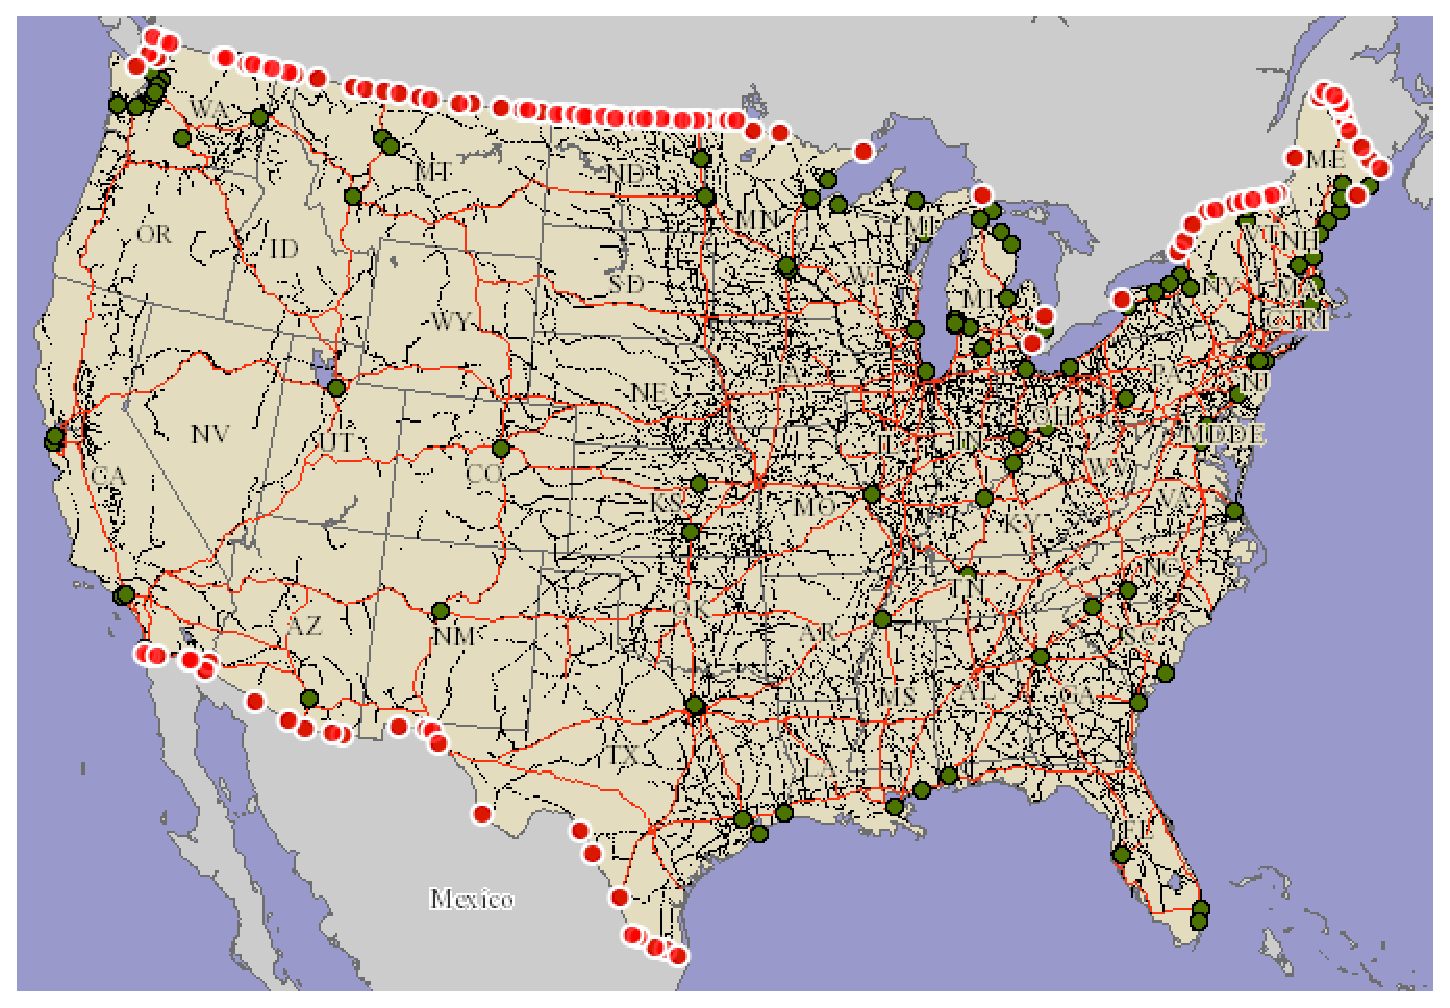
\includegraphics[width=\textwidth]{PortalEntryMap.eps}
  \end{figure}
\end{column}
\end{columns}
\end{frame}

%%%%%%%%%%%%%%%%%%%%%%%%%%%%%%%%%%%%%%%%%%%%%%%%%%%%%%%%%%%%%%%%%%%%%%%%%%%%%%%
\begin{frame}{Radiation Portal Monitors}
\begin{columns}[onlytextwidth]
	\begin{column}{0.45\textwidth}
  	\begin{itemize}
  		\item Radiation portal monitors (RPMs) are passive radiation detectors
  		\item {
  			 RPMs are currently   ${}^3$He based detectors
  			\center
    		${}^3He +n \to p +{}^3H$
    	}
  		\item Shortage of ${}^3$He, so alternatives are being explored
		  \item ${}^6Li + n \to {}^3H + \alpha$    
  		\end{itemize}
	\end{column}
	\begin{column}{0.5\textwidth}
		\begin{figure}
    \vspace*{-3cm}
      \centering
			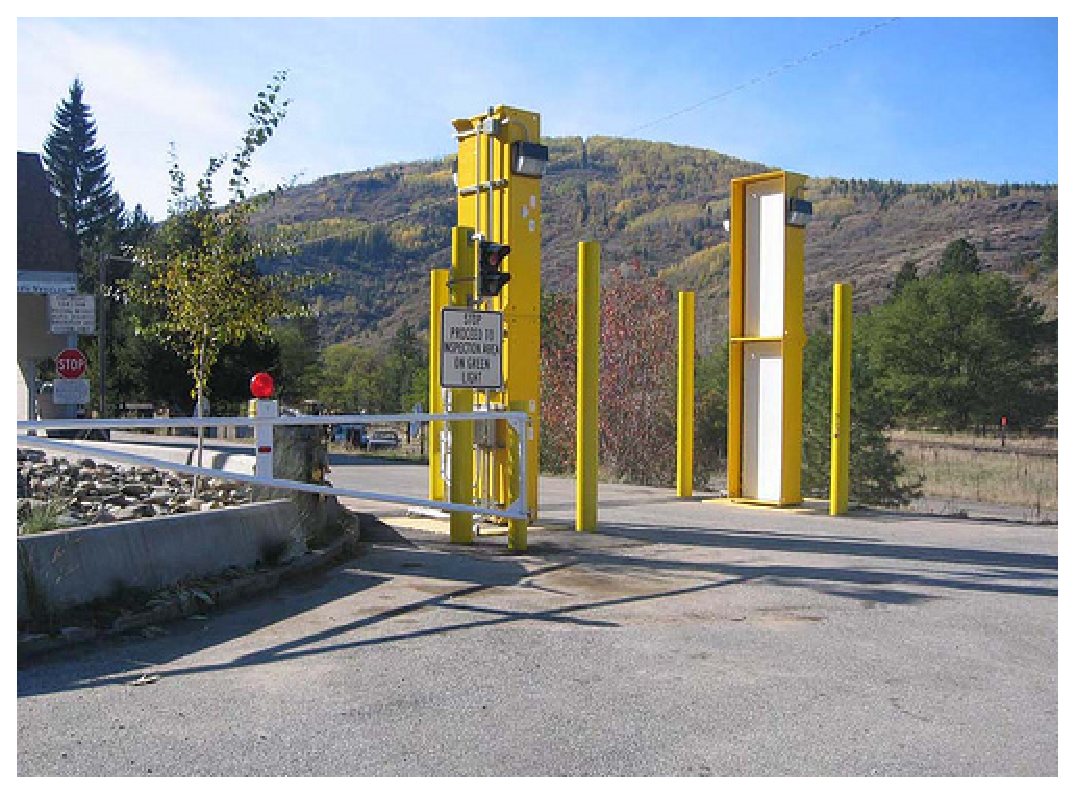
\includegraphics[width=\textwidth]{RPM8_Installed.eps}
    \end{figure}
	\end{column}
\end{columns}
\end{frame}
%%%%%%%%%%%%%%%%%%%%%%%%%%%%%%%%%%%%%%%%%%%%%%%%%%%%%%%%%%%%%%%%%%%%%%%%%%%%%%%

\subsection{Detector Requirements}
%%%%%%%%%%%%%%%%%%%%%%%%%%%%%%%%%%%%%%%%%%%%%%%%%%%%%%%%%%%%%%%%%%%%%%%%%%%%%%%
\begin{frame}{Detector Requirements}
DHS / DNDO (along with PNNL) has determined a set of objectives that replacement technologies should meet:
\begin{table}
	\small
	\begin{tabular}{ m{5cm} m{5cm} }
	Parameter & Specification \\
	\hline
	\hline
	Absolute neutron detection efficiency & 2.5 cps/ng of ${}^{252}Cf$ (in specified test configuration) \\
	Intrinsic gamma-neutron detection efficiency & $ \epsilon_{int,\gamma n}\leq 10^{-6}$ \\
	Gamma absolute rejection ratio for neutrons (GARRn) & $ 0.9 \leq \text{ GARRn }\leq$ 1.1 at 10 mR/h exposure \\
	Cost &  \$ 30,000 per system \\
	\hline
	\end{tabular}
\end{table}
\hyperlink{PNNLCriteria}{\beamerbutton{Detailed Criteria}}
\label{DHSCriteria}
\end{frame}

%%%%%%%%%%%%%%%%%%%%%%%%%%%%%%%%%%%%%%%%%%%%%%%%%%%%%%%%%%%%%%%%%%%%%%%%%%%%%%%
%                                                                             %
%                                PREVIOUS WORK                                %
%                                                                             %
%%%%%%%%%%%%%%%%%%%%%%%%%%%%%%%%%%%%%%%%%%%%%%%%%%%%%%%%%%%%%%%%%%%%%%%%%%%%%%%
\subsection{Previous Work}

%%%%%%%%%%%%%%%%%%%%%%%%%%%%%%%%%%%%%%%%%%%%%%%%%%%%%%%%%%%%%%%%%%%%%%%%%%%%%%%
\begin{frame}[fragile]{Replacement Technologies}
\begin{columns}[onlytextwidth]
\begin{column}{0.55\textwidth}
\begin{itemize}
	\small
	\item Boron Straw Tubes (Proportional Technology) \cite{kouzes_boron-lined_2012}
	\begin{itemize}
    %\tiny
		\item Count rate meets requirements
		\item Gamma rejection is estimated to be $4x10^{-9}$
		\item GARRn within desired range
	\end{itemize}
	\small
	\item LiF:ZnS coated Paddles (IAT) \cite{kouzes_lithium_2010}
	\begin{itemize}
    %\tiny
		\item Did not fulfill the neutron count rate
		\item Adequate gamma ray rejection
		\item Passed the GARRn
	\end{itemize}
\end{itemize}
\end{column}
\begin{column}{0.4\textwidth}
	\begin{figure}
    \centering
    \begin{subfigure}[b]{\textwidth}
      \centering
		  \includegraphics[height=0.25\textheight]{B10StrawFibers.eps}
      \caption{ ${}^{10}$B Straw Fibers}
      \label{fig:B10StrawFibers}
    \end{subfigure}

    \begin{subfigure}[b]{\textwidth}
      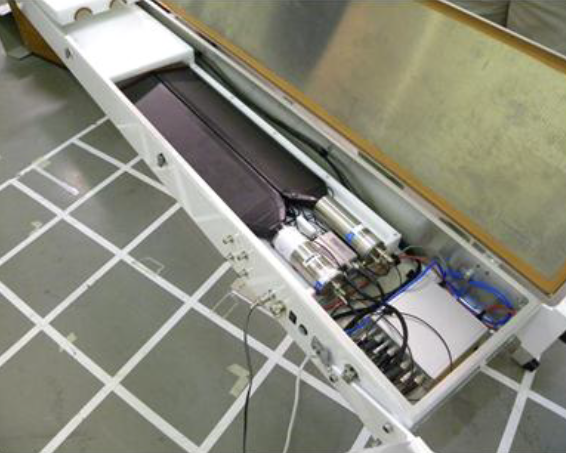
\includegraphics[height=0.25\textheight]{IATImage}
      \caption{${}^6$LiF:ZnS Paddle}
      \label{fig:LifZnSPaddle}
    \end{subfigure}
	\end{figure}
\end{column}
\end{columns}
\end{frame}

\section{Scope of Work}
\begin{frame}{Scope of Work}
  \begin{itemize}
    \item Exists a need to develop techniques and models for the performance of replacement RPMS
    \item Ability to optimize on those model is necessary
  \end{itemize}
  \begin{columns}[onlytextwidth]
    \begin{column}{0.45\textwidth}
      \begin{itemize}
        \item Maximize neutron gamma discrimination
        \item Maximize count rate per mass absorber
        \item Minimize cost of the detector
      \end{itemize}
    \end{column}
    \begin{column}{0.45\textwidth}
      \begin{itemize}
        \item Secondary electron energy deposition
        \item Neutronics simulations
        \item Light transport 
      \end{itemize}
    \end{column}
  \end{columns}
\end{frame}
%%%%%%%%%%%%%%%%%%%%%%%%%%%%%%%%%%%%%%%%%%%%%%%%%%%%%%%%%%%%%%%%%%%%%%%%%%%
%																							                            %
%																	MAIN BODY						                    %
%																							                            %
%%%%%%%%%%%%%%%%%%%%%%%%%%%%%%%%%%%%%%%%%%%%%%%%%%%%%%%%%%%%%%%%%%%%%%%%%%%
%%%%%%%%%%%%%%%%%%%%%%%%%%%%%%%%%%%%%%%%%%%%%%%%%%%%%%%%%%%%%%%%%%%%%%%%%%
%                                                                        %
%                            INTRODUCTION                                %
%                                                                        %
%%%%%%%%%%%%%%%%%%%%%%%%%%%%%%%%%%%%%%%%%%%%%%%%%%%%%%%%%%%%%%%%%%%%%%%%%%
\subsection*{}
%%%%%%%%%%%%%%%%%%%%%%%%%%%%%%%%%%%%%%%%%%%%%%%%%%%%%%%%%%%%%%%%%%%%%%%%%%
\begin{frame}[t]{Pulse Height Discrimination}
\label{PHDMain}
  \begin{itemize}
    \item Use a lower lever discriminator to discard counts
    \item Mathematical Lower Lever Discriminator (MLLD)
  \end{itemize}
  \begin{figure}
      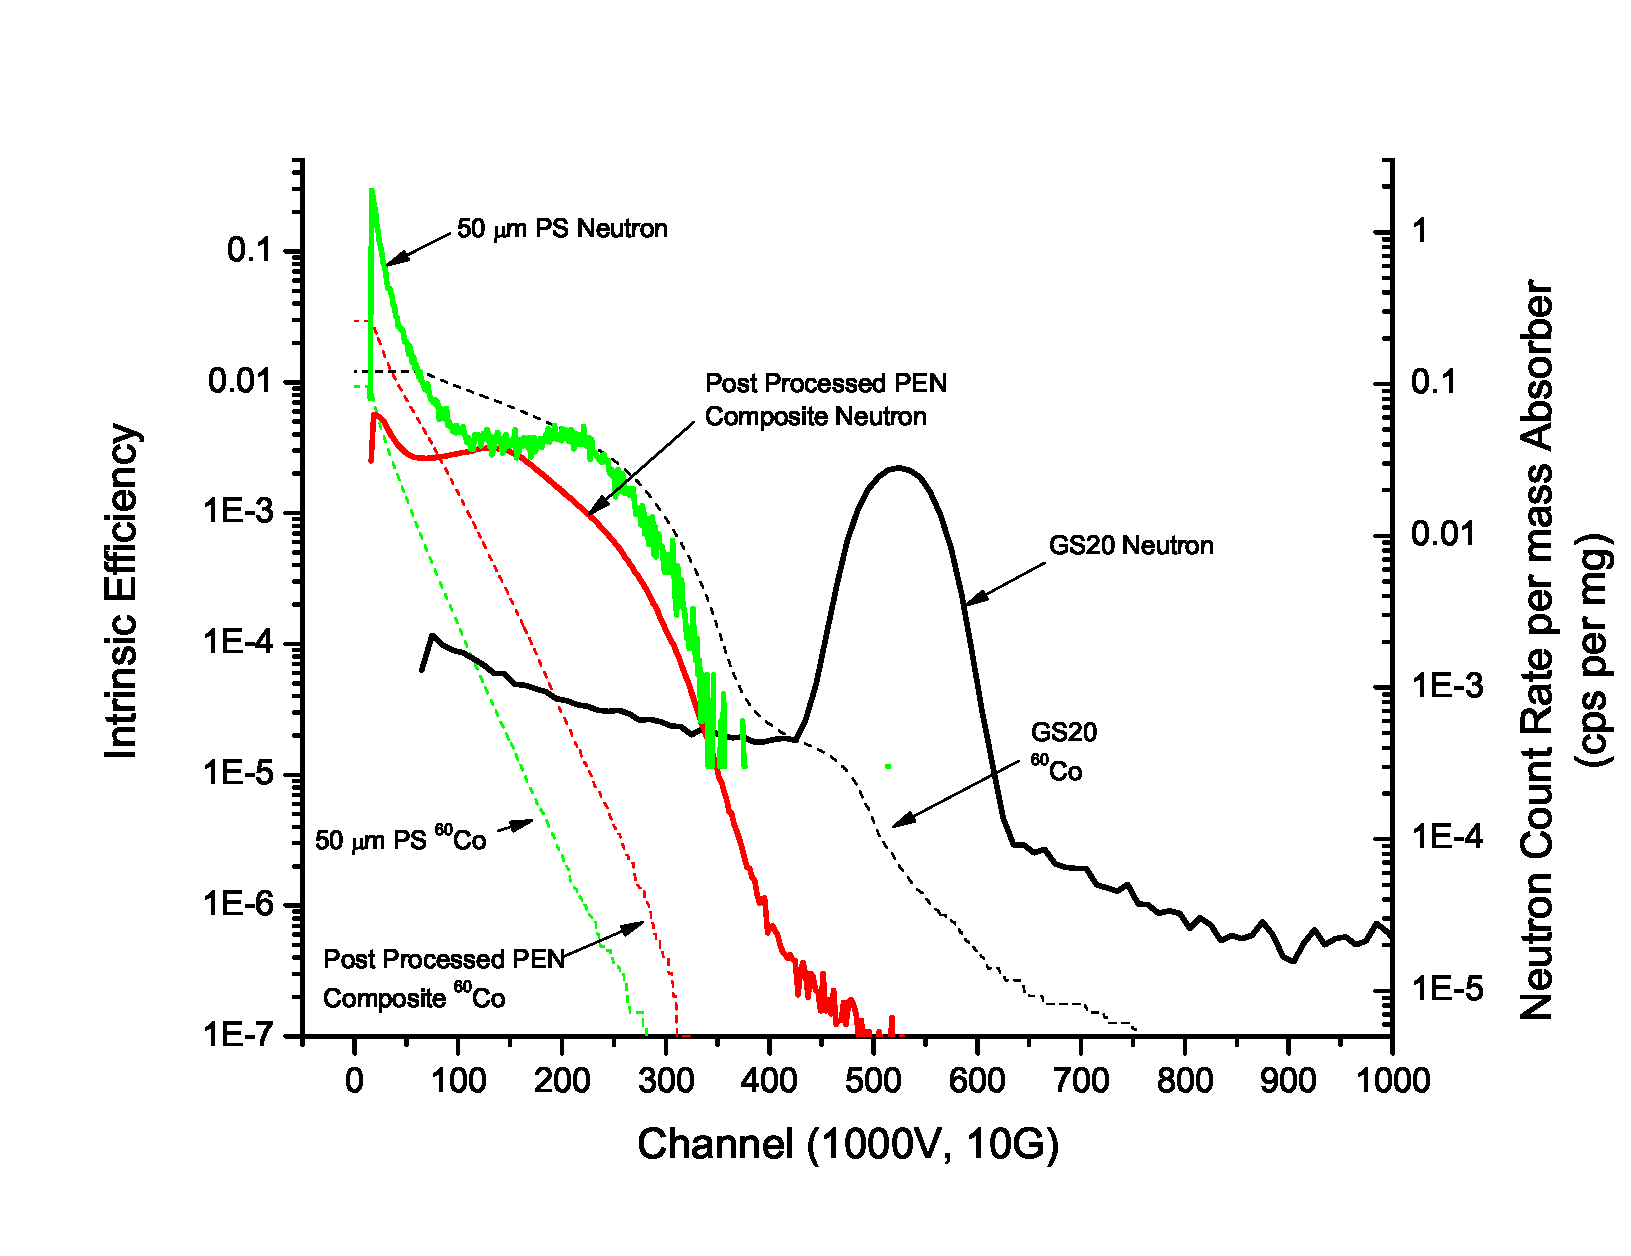
\includegraphics[height=0.6\textheight]{SC_UTDetectors_IntEff_CR}
  \end{figure}
  Pulse height discrimination is equivalent to the energy deposition
\hyperlink{MeasMethods}{\beamerbutton{Measurment Setups and Methods}}
\end{frame}
%%%%%%%%%%%%%%%%%%%%%%%%%%%%%%%%%%%%%%%%%%%%%%%%%%%%%%%%%%%%%%%%%%%%%%%%%%

\section{RPM Neutronics}
%%%%%%%%%%%%%%%%%%%%%%%%%%%%%%%%%%%%%%%%%%%%%%%%%%%%%%%%%%%%%%%%%%%%%%%%%%
%                                                                        %
%                            INTRODUCTION                                %
%                                                                        %
%%%%%%%%%%%%%%%%%%%%%%%%%%%%%%%%%%%%%%%%%%%%%%%%%%%%%%%%%%%%%%%%%%%%%%%%%%
\subsection*{}
\begin{frame}{Introduction}
  \large
  \centering{Will a candidate detector work?}
  \vspace{1cm}
  \normalsize
  \begin{itemize}
    \item Modeling is needed to simulate large area plastic
    \item MCNPX is a well validated transport code
    \begin{itemize}
        \item MCNPX is a Monte Carlo based
        \item MCNPX has drawbacks with energy deposition
    \end{itemize}
    \item Previous work has shown that it is possible to model detector neutronics with MCNPX
  \end{itemize}
\end{frame}
%%%%%%%%%%%%%%%%%%%%%%%%%%%%%%%%%%%%%%%%%%%%%%%%%%%%%%%%%%%%%%%%%%%%%%%%%%
\begin{frame}{Multi Film Model}
	\begin{figure}
    \vspace*{-9cm}
    \begin{subfigure}[b]{0.47\textwidth}
      \centering
      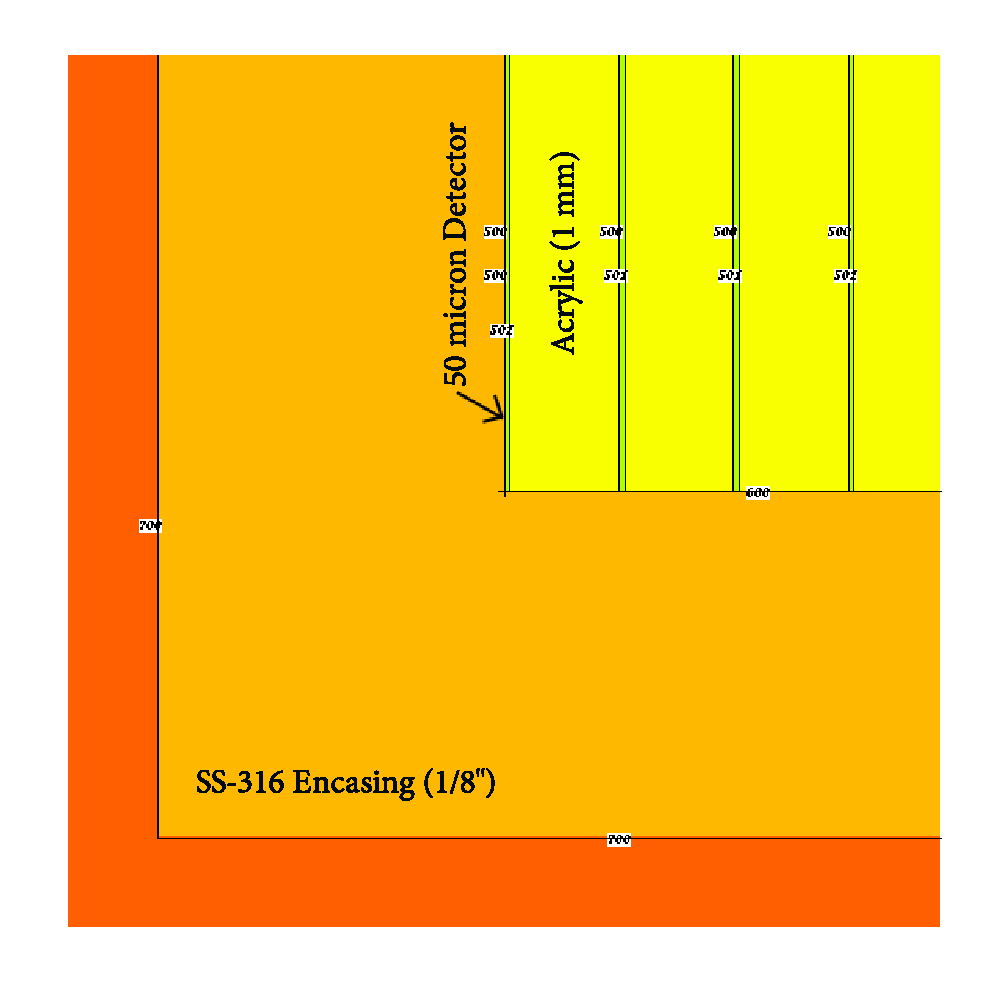
\includegraphics[width=\textwidth]{Multi_120Layers.eps}
      \caption{Simulated RPM8 Detector (120 layers)}
    \end{subfigure}
    ~
    \begin{subfigure}[b]{0.47\textwidth}
      \centering
      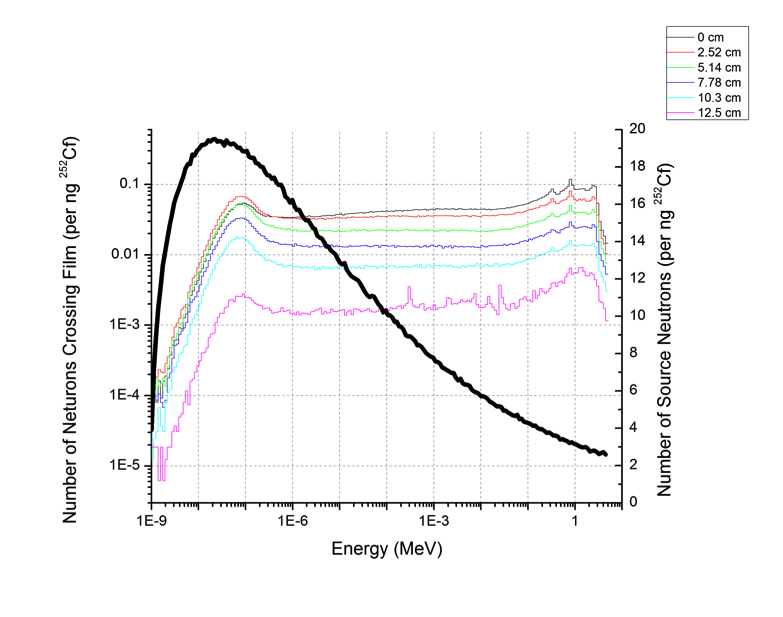
\includegraphics[width=2\textwidth]{Spectra_Layered.eps}
      \caption{Source and Incident Spectra}
    \end{subfigure}
	\end{figure}
\end{frame}
%%%%%%%%%%%%%%%%%%%%%%%%%%%%%%%%%%%%%%%%%%%%%%%%%%%%%%%%%%%%%%%%%%%%%%%%%%
\begin{frame}{Opportunities for Optimization}
  \begin{columns}[onlytextwidth]
    \begin{column}{0.45\textwidth}
    \begin{itemize}
      \item Neutron absorber loading of the film
      \item Thickness of the film
      \item Geometry of the film
      \item Placement of the films
    \end{itemize}
    \end{column}
    \begin{column}{0.45\textwidth}
      \begin{figure}
        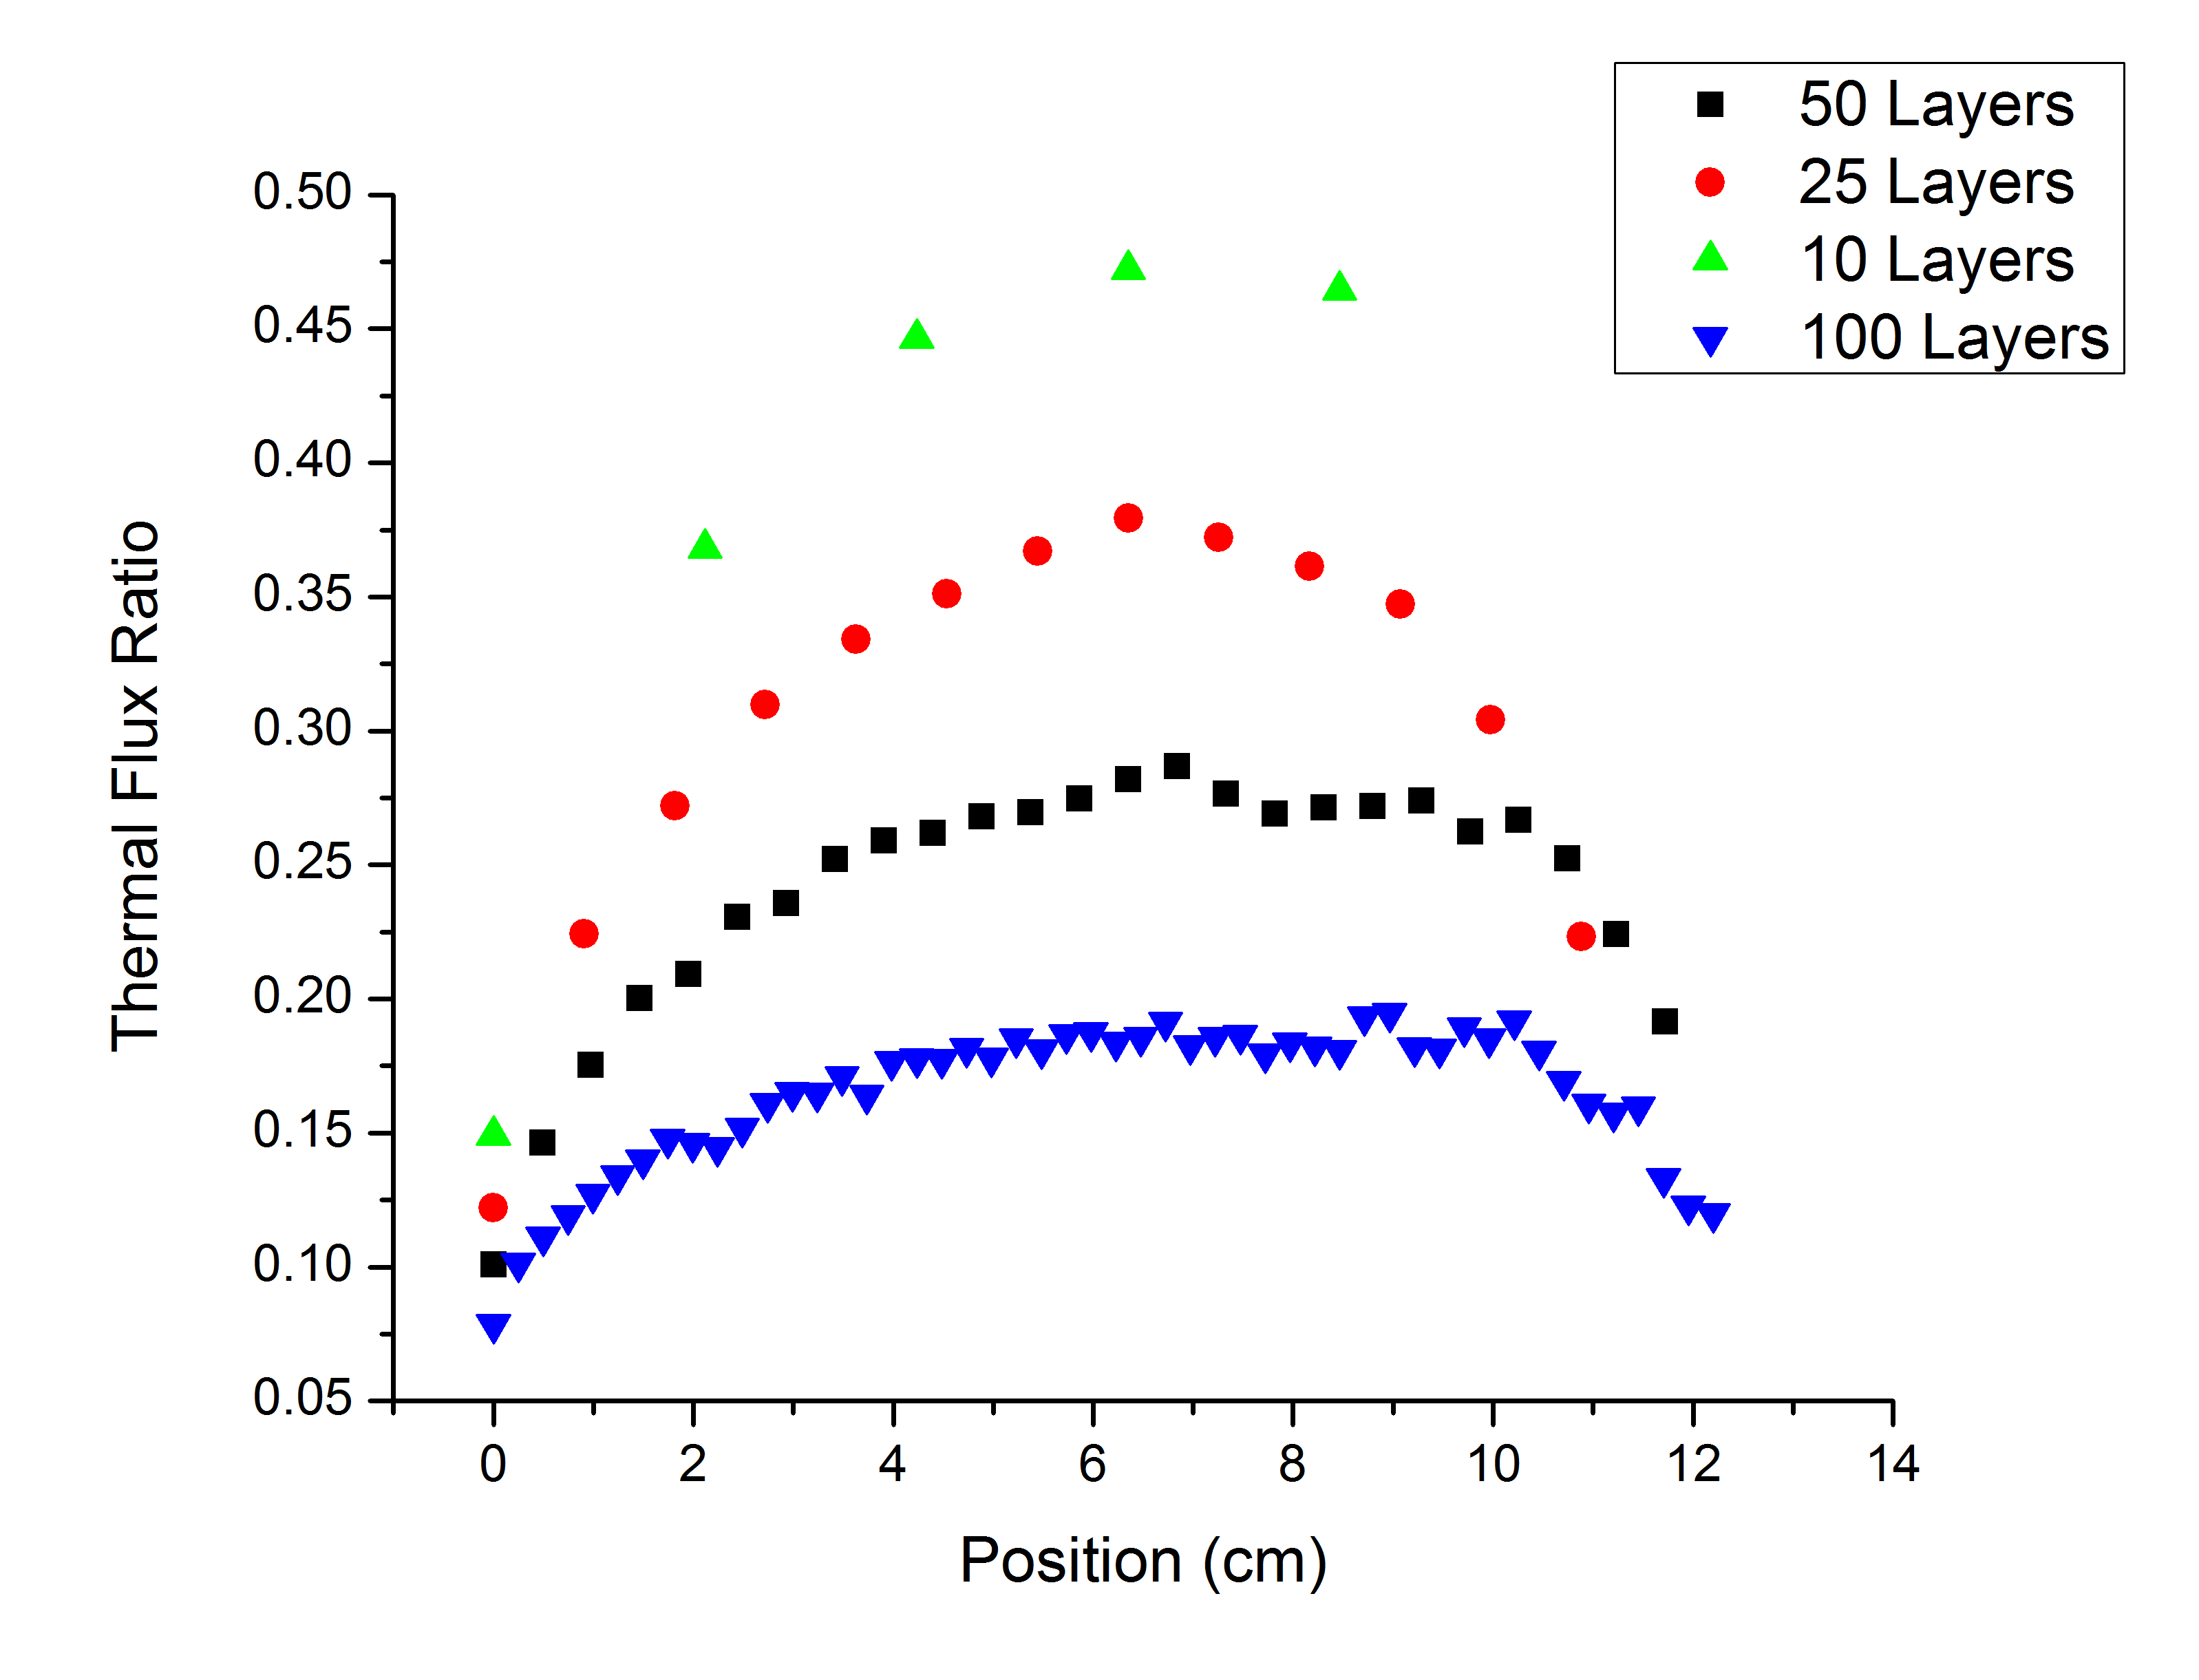
\includegraphics[width=\textwidth]{ThermalFluxRatioAltLayers}
      \end{figure}
    \end{column}
  \end{columns}
\end{frame}
%%%%%%%%%%%%%%%%%%%%%%%%%%%%%%%%%%%%%%%%%%%%%%%%%%%%%%%%%%%%%%%%%%%%%%%%%%
%                                                                        %
%                             PROPOSED WORK                              %
%                                                                        %
%%%%%%%%%%%%%%%%%%%%%%%%%%%%%%%%%%%%%%%%%%%%%%%%%%%%%%%%%%%%%%%%%%%%%%%%%%
\subsection{Proposed Work}
\begin{frame}{Proposed Work}
  \large
  \textbf{Optimization of the film placement}
  \normalsize
  \begin{itemize}
    \item Focus on minimizing amount of \iso[6]{Li} while meeting criteria
    \begin{itemize}
      \item Search the parameter space of possible detector designs
      \item Study effects of self-shielding and different geometries
    \end{itemize}
  \end{itemize}
\textbf{What do we mean by best?}
\begin{itemize}
	\small
  \item Count rate? 
  \item Light output?
	\item Lowest cost / fabrication ease?
\end{itemize}
\textbf{The design parameters were then:}
\begin{itemize}
	\small
  \item The detector material
  \item The thickness of the detector material
  \item The spacing of detector layers
\end{itemize}
\end{frame}
%%%%%%%%%%%%%%%%%%%%%%%%%%%%%%%%%%%%%%%%%%%%%%%%%%%%%%%%%%%%%%%%%%%%%%%%%%
%                                                                        %
%                               METHODS                                  %
%                                                                        %
%%%%%%%%%%%%%%%%%%%%%%%%%%%%%%%%%%%%%%%%%%%%%%%%%%%%%%%%%%%%%%%%%%%%%%%%%%
\subsection{Methods}
\begin{frame}[fragile]
\frametitle{Neutron Interaction Rate}
	\tiny
	\newtheorem{thm11}{Interaction Rate}
	\begin{thm11}<1->
		$$Q = C \int {\Phi(E) R_m(E) dE }$$
	where:
	\begin{itemize}
		\item $C$ is a scalar normalization (density)
		\item $R_m(E)$ is the response function
		\item $\Phi(E)$ is the neutron flux
	\end{itemize}
	\end{thm11}
Accomplished using a F4 tally with multiplier
\tiny
\begin{lstlisting}
c -------- Interaction Rate Tallies -------------
FC154 (n,t) Reactions in Detector
F154:n (601<610) (602<610) (603<610) (604<610) T
FM154 -1 3 105
\end{lstlisting}
\end{frame}
%%%%%%%%%%%%%%%%%%%%%%%%%%%%%%%%%%%%%%%%%%%%%%%%%%%%%%%%%%%%%%%%%%%%%%%%%%
\begin{frame}[fragile]{Gigantic Genome Geometries}
\label{GAMethod}
Genome Bit-String Representation
\begin{itemize}
  \item Divide the RPM8 width into even slices
  \item Compact representation of geometry, suitable for GA
  \item \verb+1+ - represents a detector assembly slice
  \item \verb+0+ - represents a moderator slice
  \item Example: \verb+001000+
  \begin{itemize}
    \item Each slice is \SI{2.12}{\centi\meter}
    \item Two slices of moderator, followed by one assembly slice followed by three additional slices of moderator
  \end{itemize}
\end{itemize}
\hyperlink{GAMethodExtended}{\beamerbutton{Detailed GA Introduction}}
\end{frame}
%%%%%%%%%%%%%%%%%%%%%%%%%%%%%%%%%%%%%%%%%%%%%%%%%%%%%%%%%%%%%%%%%%%%%%%%%%
\begin{frame}{Example Geometry}
\begin{columns}[onlytextwidth]
  \begin{column}{0.45\textwidth}
    \small
    \begin{itemize}
      \item Population of candidate solutions is evolved toward better solutions
      \item Each candidate has properties that can be mutated and altered
      \item Traditionally solutions are represented as bit strings or trees
    \end{itemize}
    \end{column}
  \begin{column}{0.45\textwidth}
    \begin{figure}
		\tiny
    \end{figure}
  \end{column}
\end{columns}
\hyperlink{GAMethodExtended}{\beamerbutton{Detailed GA Introduction}}
\end{frame}
%%%%%%%%%%%%%%%%%%%%%%%%%%%%%%%%%%%%%%%%%%%%%%%%%%%%%%%%%%%%%%%%%%%%%%%%%%
%                                                                        %
%                          PRELIMARY RESULTS                             %
%                                                                        %
%%%%%%%%%%%%%%%%%%%%%%%%%%%%%%%%%%%%%%%%%%%%%%%%%%%%%%%%%%%%%%%%%%%%%%%%%%
\subsection{Preliminary Results}
%%%%%%%%%%%%%%%%%%%%%%%%%%%%%%%%%%%%%%%%%%%%%%%%%%%%%%%%%%%%%%%%%%%%%%%%%%
\begin{frame}{Optimal Geometries Rendered}
\begin{figure}
    \centering
    \begin{subfigure}[b]{0.45\textwidth}
        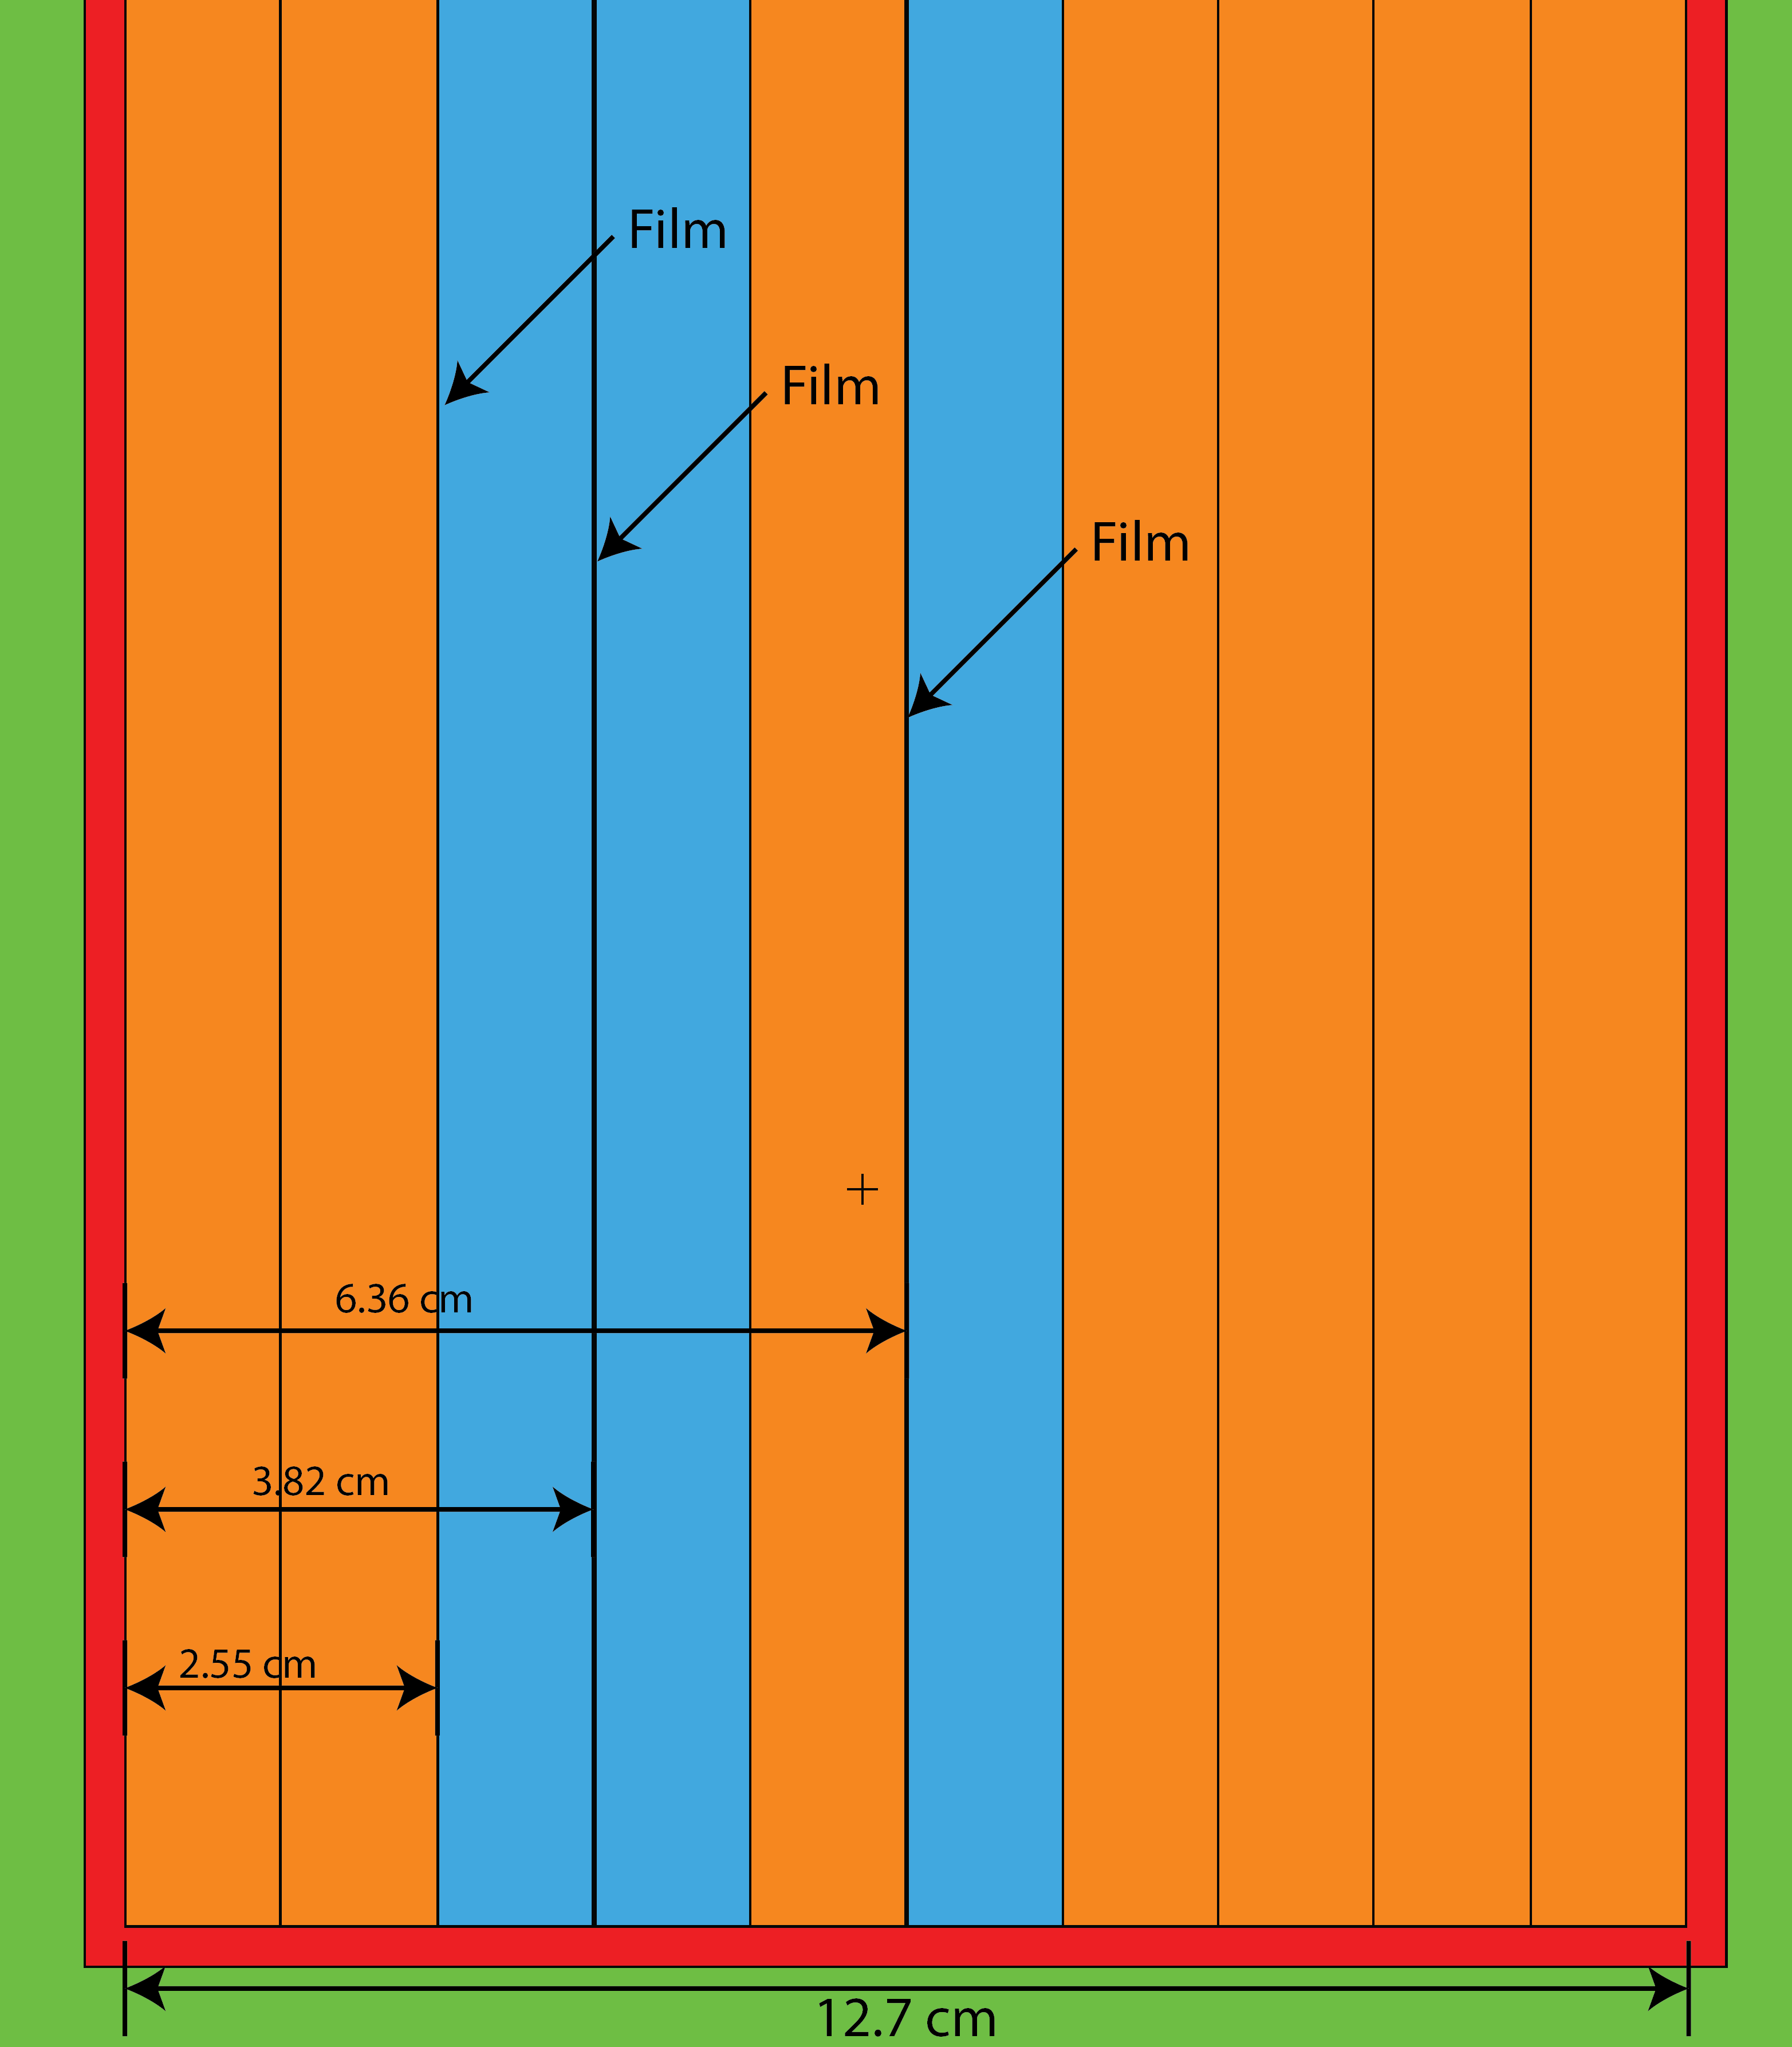
\includegraphics[width=\textwidth]{RPM8OptLayered_25cps}
    \end{subfigure}%
    ~
    \begin{subfigure}[b]{0.45\textwidth}
        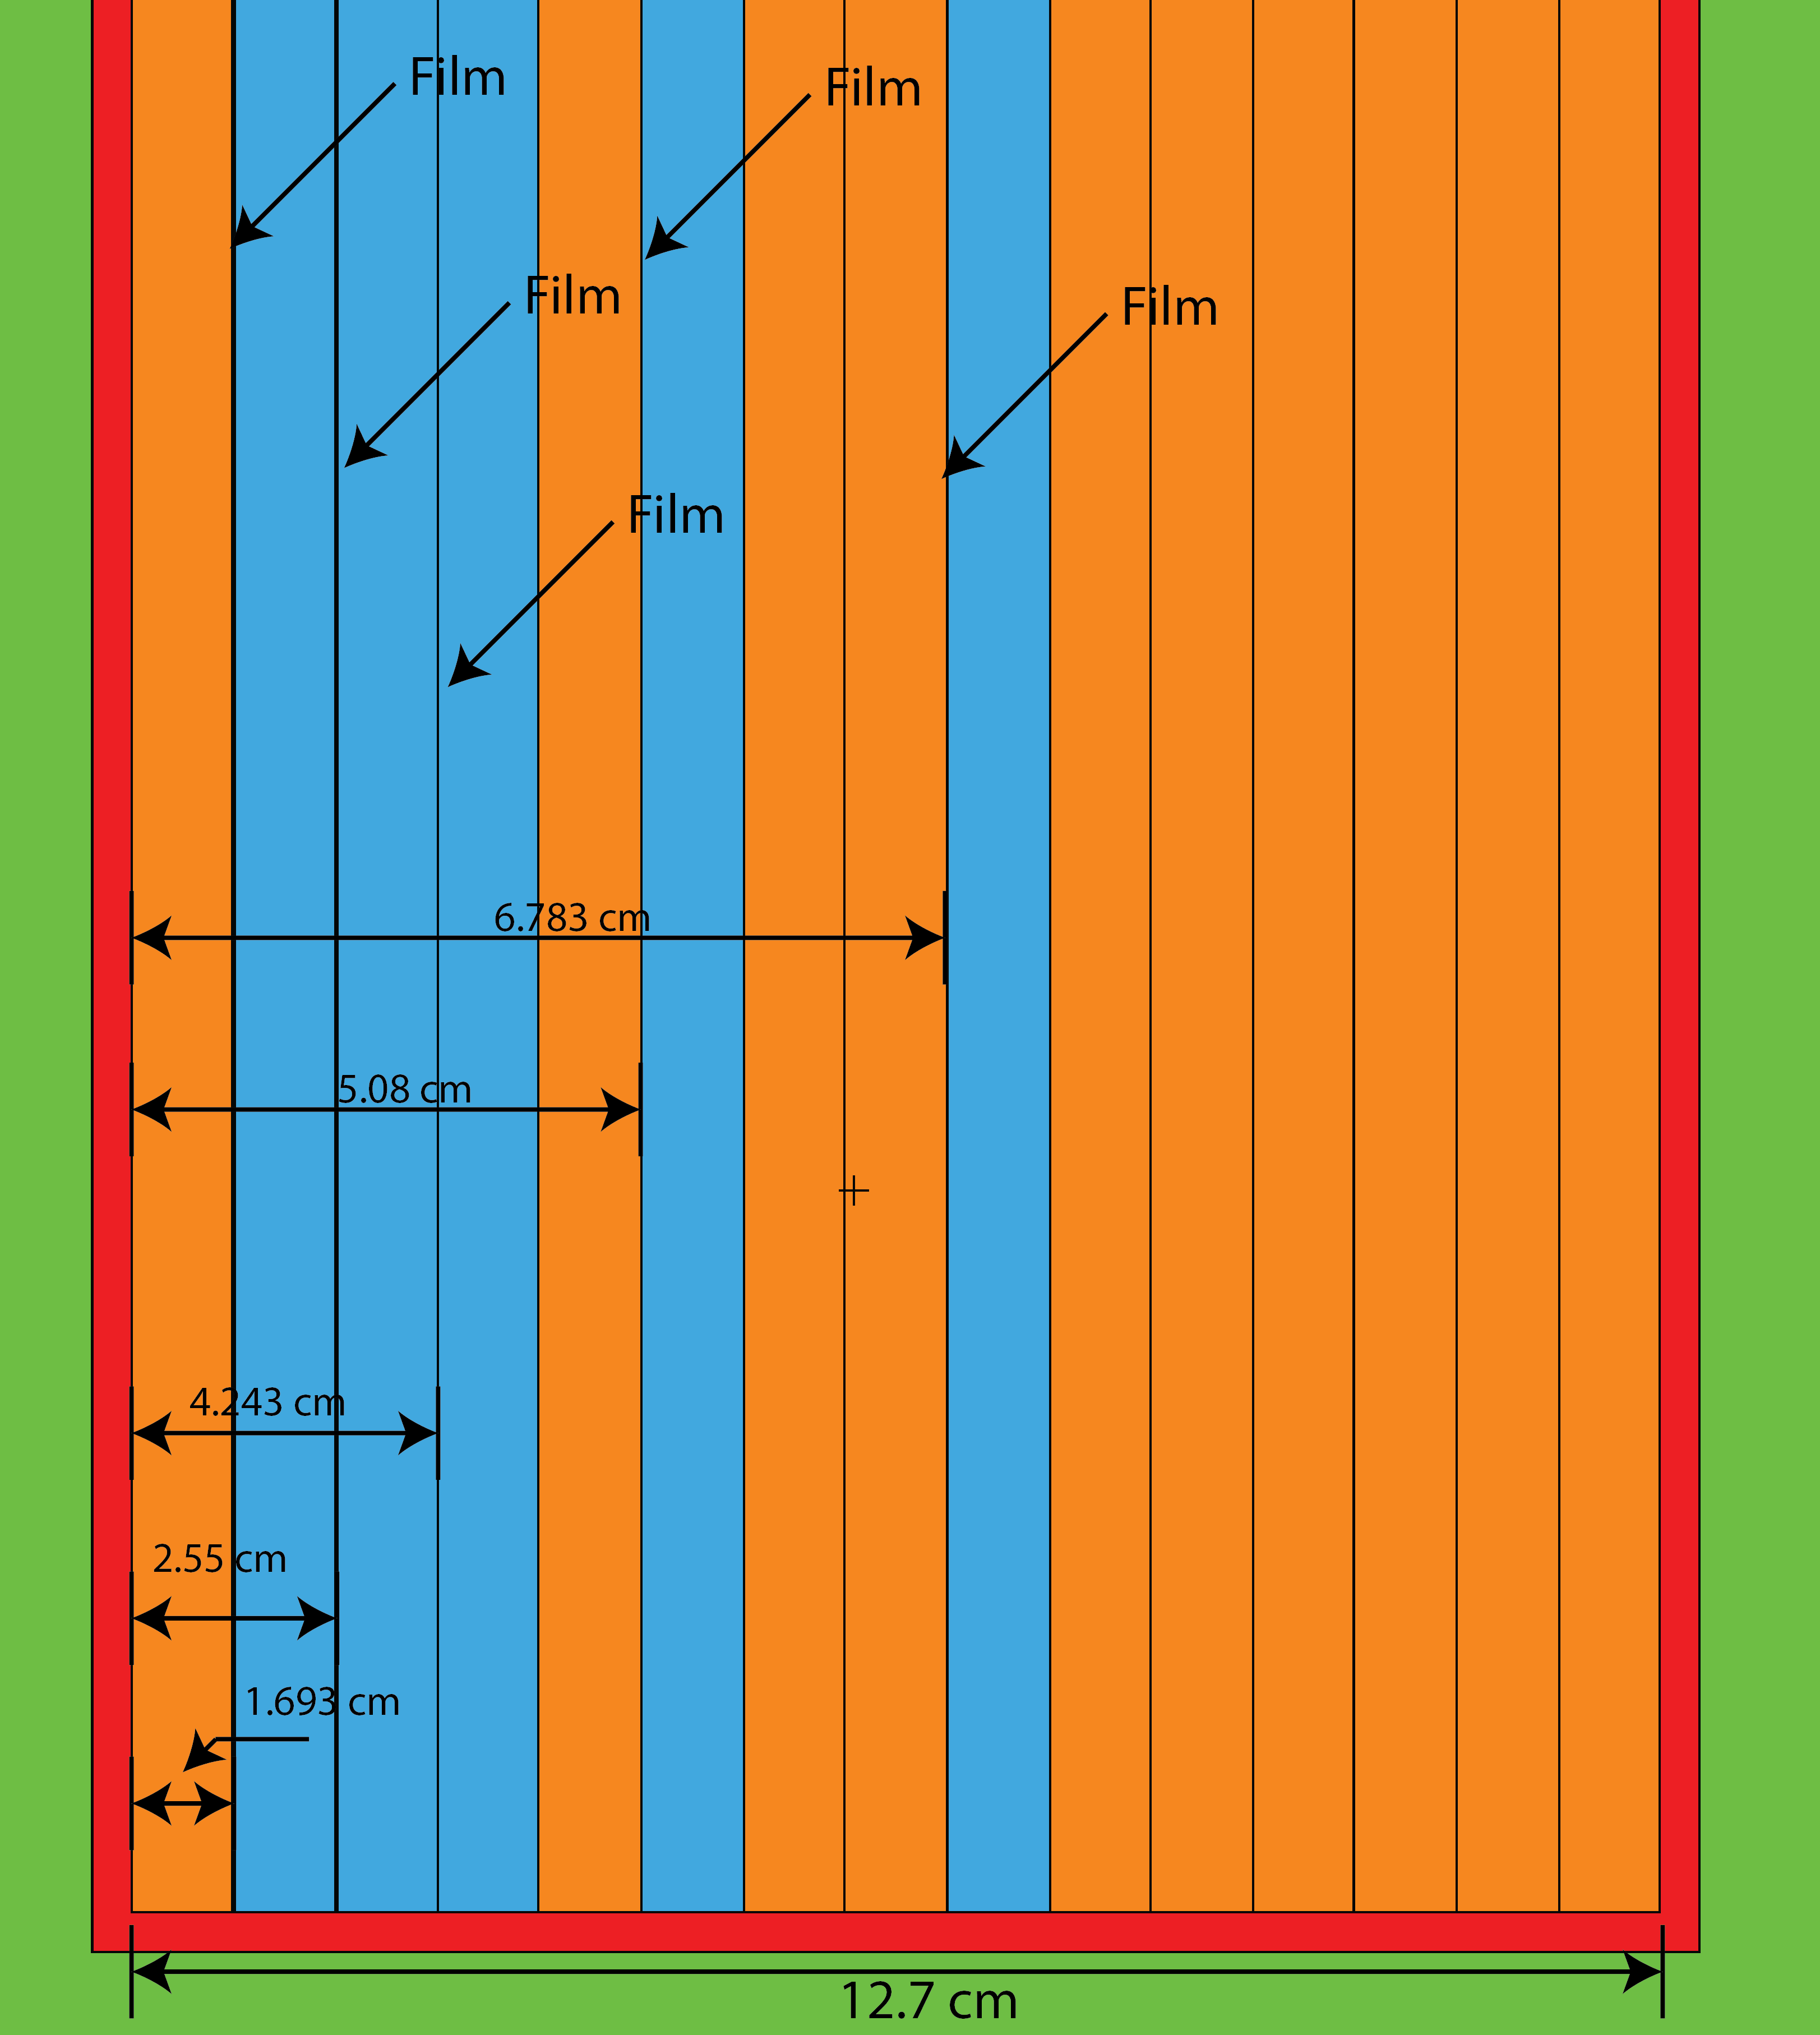
\includegraphics[width=\textwidth]{RPM8OptLayered_5cps}
    \end{subfigure}
    \caption{MCNPX rendering of layered geometry}
    \label{fig:MCNPXRendering}
\end{figure}
\end{frame}
%%%%%%%%%%%%%%%%%%%%%%%%%%%%%%%%%%%%%%%%%%%%%%%%%%%%%%%%%%%%%%%%%%%%%%%%%%
\begin{frame}[fragile]{Optimal Geometries}
\begin{table}
    %\caption[Optimal Bit String Geometries]{Genatic Algothrim Optimal Geometries}
    \centering
    \tiny
    \begin{tabular}{ p{0.75cm} | p{1cm} p{3.25cm} p{0.75cm} p{1cm} p{1cm}}
      Genome Length&Films Per Assembly&Optimal Geometry&Mass \iso[6]{Li}(g)&CPS per ng \iso[252]{Cf} & Count Rate per Mass \iso[6]{Li} (cps/g) \\
      \hline
      \hline
      3&4&\verb+010+&16.75&2.93&0.175 \\
      4&4&\verb+0100+& & & \\
      5&3&\verb+01000+&12.56&2.89&0.230 \\
      6&3&\verb+010000+&12.56&2.88&0.230 \\
      7&3&\verb+0100000+&12.56&2.84&0.226 \\ 
      10&3&\verb+0100000000+&12.56&2.68&0.214 \\
      10&3&\verb+0010000000+&12.56&2.93&0.233 \\
      10&3&\verb+0001000000+&12.56&2.95&0.235 \\
      13&2&\verb+00010010000000+&16.75&3.88&0.232 \\
      13&2&\verb+00100010000000+&16.75&3.90&0.233 \\
      13&2&\verb+00100100000000+&16.75&3.87&0.231 \\
      26&1&\verb+00000110110000000010000000+&20.94&4.33&0.206 \\
      26&1&\verb+00001010001000100000000000+&16.75&4.20&0.251 \\
    \end{tabular}
\end{table}
\end{frame}

\section{Energy Deposition}
%%%%%%%%%%%%%%%%%%%%%%%%%%%%%%%%%%%%%%%%%%%%%%%%%%%%%%%%%%%%%%%%%%%%%%%%%%
%                                                                        %
%                            INTRODUCTION                                %
%                                                                        %
%%%%%%%%%%%%%%%%%%%%%%%%%%%%%%%%%%%%%%%%%%%%%%%%%%%%%%%%%%%%%%%%%%%%%%%%%%
\subsection*{}
\begin{frame}{Neutron - Gamma Discrimination}
  \begin{columns}[onlytextwidth]
    \begin{column}{0.45\textwidth}
    \large
    Methods of Neutron - Gamma Discrimination
    \normalsize
    \begin{itemize}
      \item Pulse shape 
      \item Pulse height
      \item Limit interactions
    \end{itemize}
    \end{column}
    \begin{column}{0.45\textwidth}
      How thick does a detector need to be to have less than one in a million interactions?
      \vspace{1cm}
      \begin{align*}
        \num{1E-6} &\le 1-\exp\left ( \frac{-\mu}{\rho}t \right )  
      \end{align*}
      \pause
      \huge
      \textcolor{red}{160 nm}
    \end{column}
  \end{columns}
\end{frame}
%%%%%%%%%%%%%%%%%%%%%%%%%%%%%%%%%%%%%%%%%%%%%%%%%%%%%%%%%%%%%%%%%%%%%%%%%%
\begin{frame}[t]{Pulse Height Discrimination}
  \begin{itemize}
    \item Use a lower lever discriminator to discard counts
    \item Mathematical Lower Lever Discriminator (MLLD)
  \end{itemize}
  \begin{columns}[onlytextwidth]
    \begin{column}{0.7\textwidth}
      \begin{figure}
          \vspace*{-1cm}
          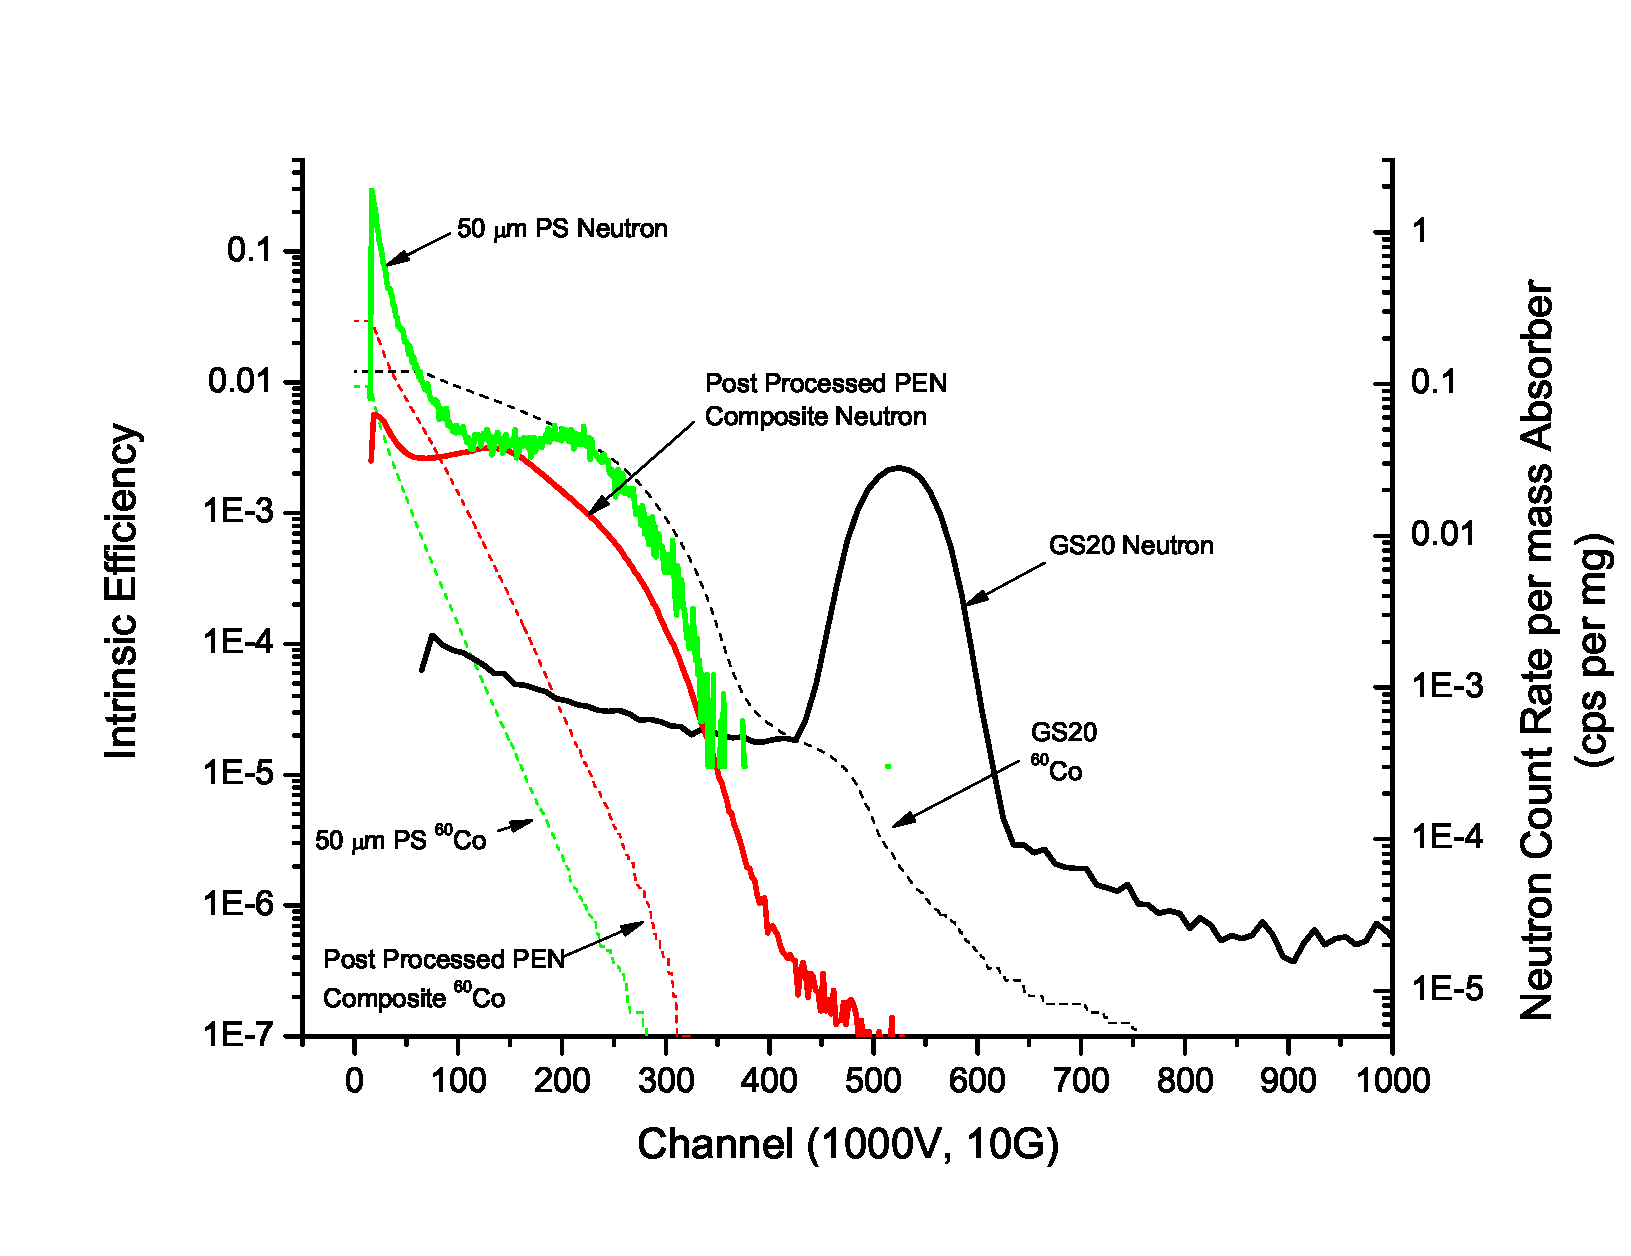
\includegraphics[width=\textwidth]{SC_UTDetectors_IntEff_CR}
      \end{figure}
    \end{column}
    \begin{column}{0.25\textwidth}
  \begin{align*}
    \frac{dL}{dx} = \frac{S_B\frac{dE}{dx}}{1+kB\frac{dE}{dx}}
  \end{align*}
    \end{column}
  \end{columns}
  Pulse height discrimination is equivalent to the energy deposition
\end{frame}
%%%%%%%%%%%%%%%%%%%%%%%%%%%%%%%%%%%%%%%%%%%%%%%%%%%%%%%%%%%%%%%%%%%%%%%%%%
%                                                                        %
%                             PROPOSED WORK                              %
%                                                                        %
%%%%%%%%%%%%%%%%%%%%%%%%%%%%%%%%%%%%%%%%%%%%%%%%%%%%%%%%%%%%%%%%%%%%%%%%%%
\subsection{Proposed Work}
\begin{frame}{Proposed Work}
  \large
  \centering{What is the optimal detector thickness?}
  \vspace{1cm}
  \normalsize
  \begin{itemize}
    \item Use GEANT4 to study the energy deposition in polymeric films
    \small
    \begin{itemize}
      \item How much energy is from the alpha, triton?
      \item How many and energy distribution of secondary electrons from neutrons, gammas
    \end{itemize}
    \item GEANT4 Simulations
    \begin{itemize}
      \item Single collision energy loss spectra
      \item Ranges of alpha, triton in material
      \item Simulated Spectra
    \end{itemize}
    \item Validate simulations with measurements
  \end{itemize}
\end{frame}
%%%%%%%%%%%%%%%%%%%%%%%%%%%%%%%%%%%%%%%%%%%%%%%%%%%%%%%%%%%%%%%%%%%%%%%%%%
%                                                                        %
%                               METHODS                                  %
%                                                                        %
%%%%%%%%%%%%%%%%%%%%%%%%%%%%%%%%%%%%%%%%%%%%%%%%%%%%%%%%%%%%%%%%%%%%%%%%%%
\subsection{Methods}
\begin{frame}[fragile]{GEANT4 Introduction}
What GEANT4 is:
\begin{itemize}
  \small
  \item \href{geant4.cern.ch}{geant4.cern.ch}
  \item Free software package for the simulation of the passage of particles through matter
  \item Essentially a collection of tools for geometry, materials, physics models, events and digitization, visualizations $\dots$
  \item Maintained by the CERN community, widely used in physics
\end{itemize}
What GEANT4 is not:
\begin{itemize}
  \small
  \item For the timid
  \begin{itemize}
    \item Users are responsible for correctly implementing their own physics
    \item Users are responsible for correctly implementing their own analysis
  \end{itemize}
  \item Stagnant - major release are still occurring
\end{itemize}
\end{frame}
%%%%%%%%%%%%%%%%%%%%%%%%%%%%%%%%%%%%%%%%%%%%%%%%%%%%%%%%%%%%%%%%%%%%%%%%%%
%                                                                        %
%                          PRELIMARY RESULTS                             %
%                                                                        %
%%%%%%%%%%%%%%%%%%%%%%%%%%%%%%%%%%%%%%%%%%%%%%%%%%%%%%%%%%%%%%%%%%%%%%%%%%
\subsection{Preliminary Results}
\begin{frame}{Single Collision Energy Loss Spectra}
  \begin{figure}
    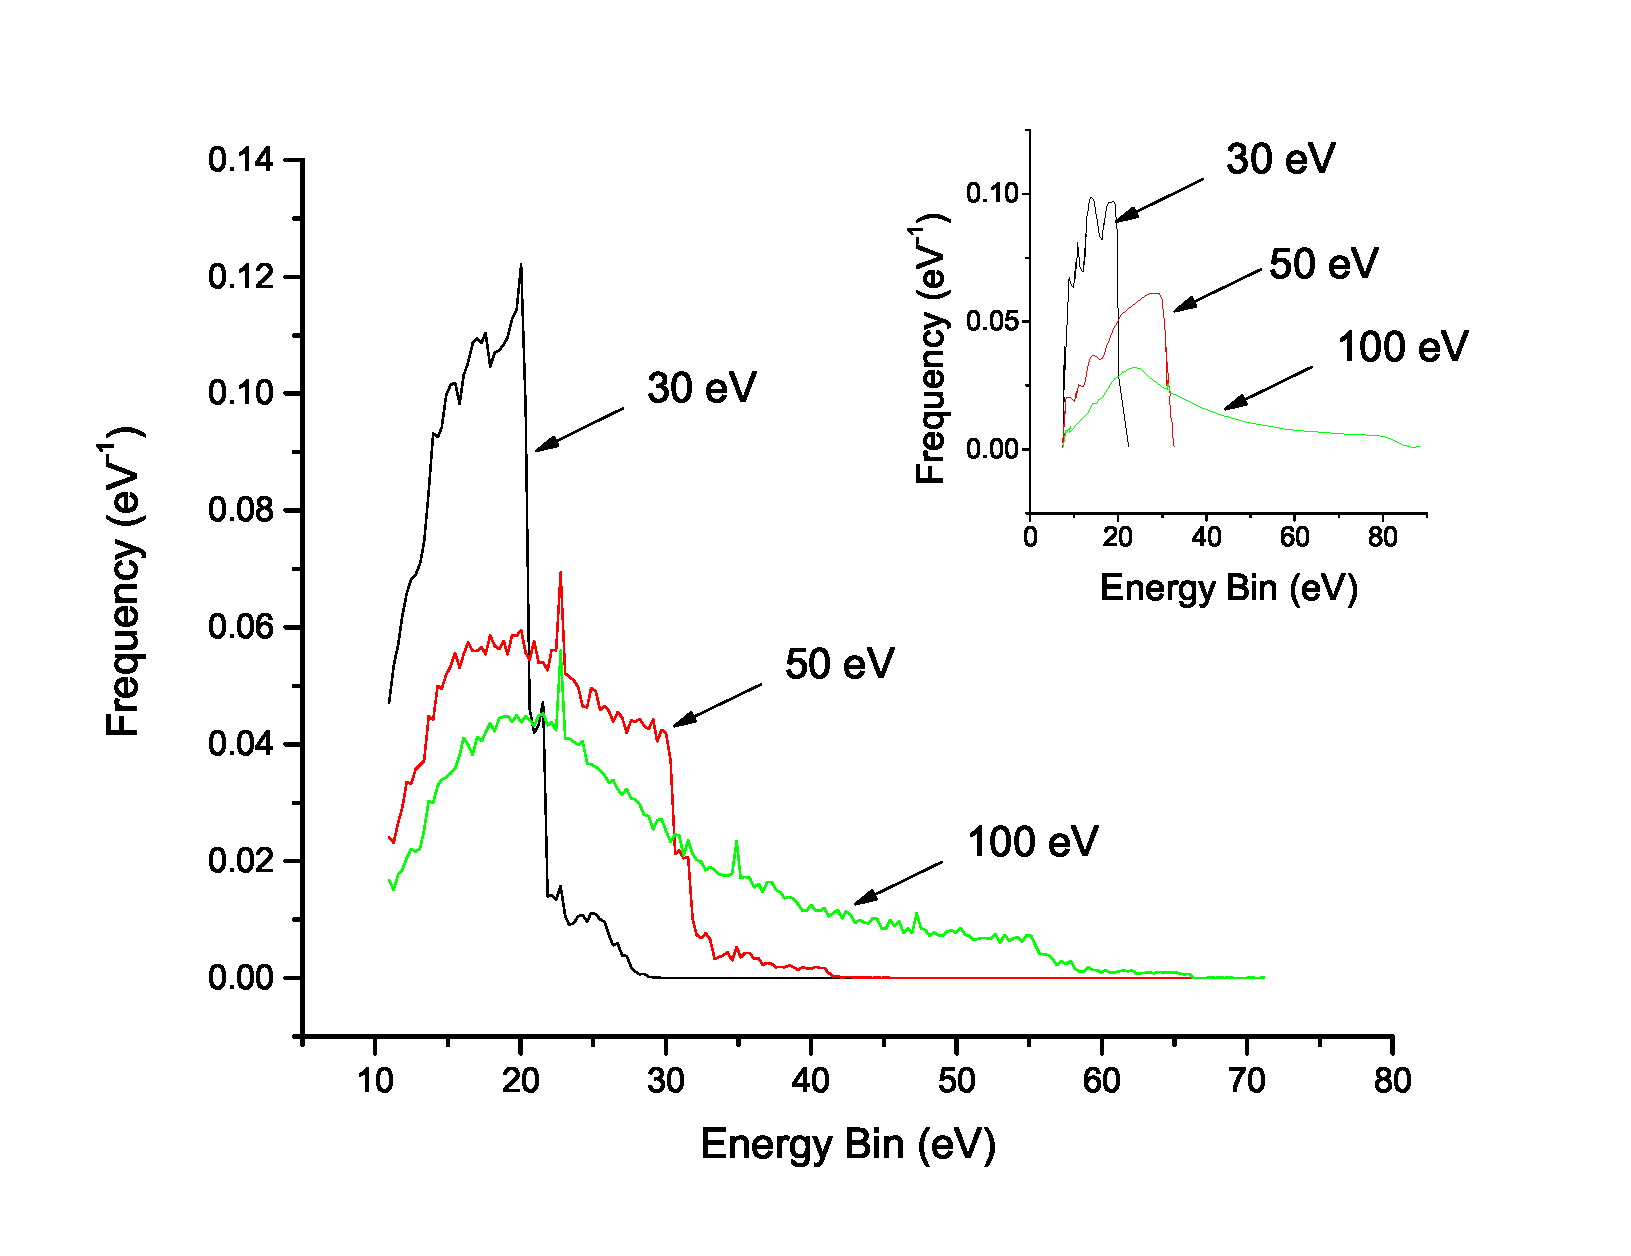
\includegraphics[width=\textwidth]{SingleCollsionEnergyLoss_Turner}
    \caption{Single Collision Energy Loss in Water\cite{turner_comparative_1982}}
  \end{figure}
\vspace{2mm}
Discrepancies are in the resolution of cross section data
\end{frame}
%%%%%%%%%%%%%%%%%%%%%%%%%%%%%%%%%%%%%%%%%%%%%%%%%%%%%%%%%%%%%%%%%%%%%%%%%%
\begin{frame}{Example Event}
  \begin{figure}
    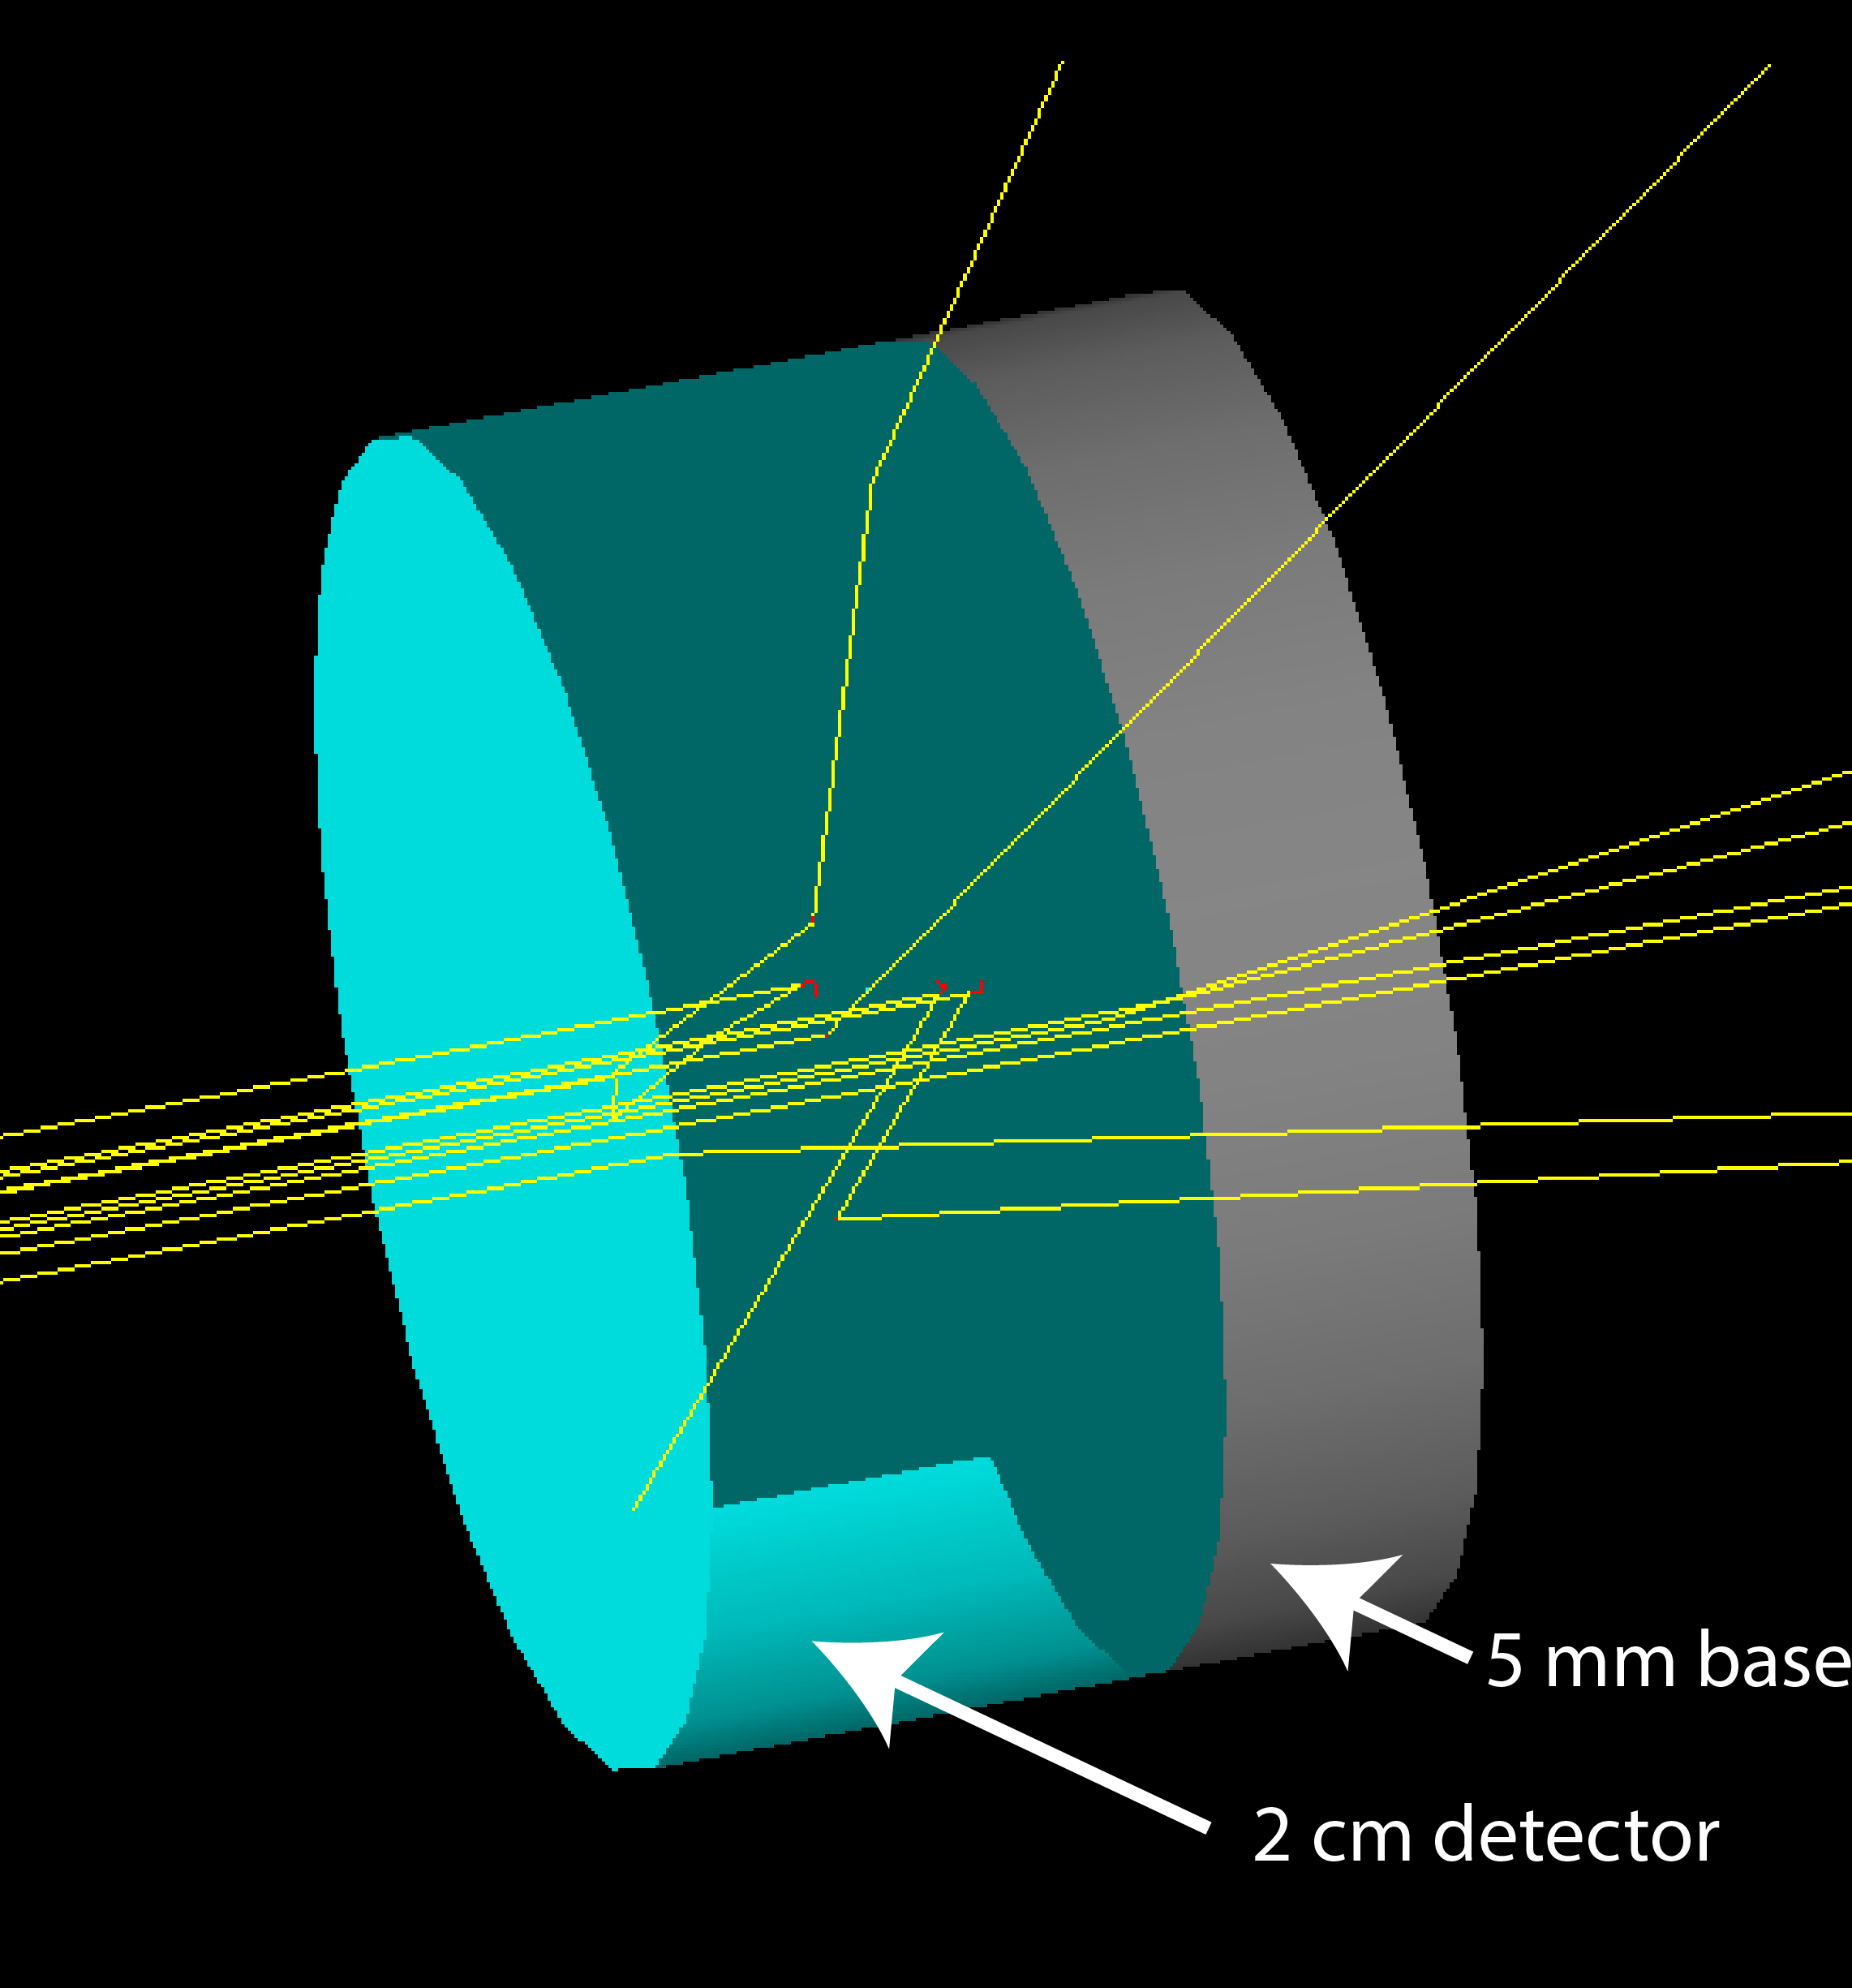
\includegraphics[height=0.75\textheight]{GEANT4AnnotatedGeo_EnergyDepEvent}
  \end{figure}
\end{frame}
%%%%%%%%%%%%%%%%%%%%%%%%%%%%%%%%%%%%%%%%%%%%%%%%%%%%%%%%%%%%%%%%%%%%%%%%%%

\section{Light Transport}
%%%%%%%%%%%%%%%%%%%%%%%%%%%%%%%%%%%%%%%%%%%%%%%%%%%%%%%%%%%%%%%%%%%%%%%%%%
%                                                                        %
%                            INTRODUCTION                                %
%                                                                        %
%%%%%%%%%%%%%%%%%%%%%%%%%%%%%%%%%%%%%%%%%%%%%%%%%%%%%%%%%%%%%%%%%%%%%%%%%%
\subsection*{}
\begin{frame}{Ability to Detect Signal}
  \textbf{How is the light collected from the detector}
  \vspace{1cm}
  \begin{itemize}
    \item Not all of the detectors are optically transparent
    \item Light collection strategies:
    \begin{itemize}
      \item Pipe the light out along the edge?
      \item Use wavelength shifters?
      \item How much spacing is needed between layers?
    \end{itemize}
    \item Is it possible to design a workable detector?
  \end{itemize}
\end{frame}
%%%%%%%%%%%%%%%%%%%%%%%%%%%%%%%%%%%%%%%%%%%%%%%%%%%%%%%%%%%%%%%%%%%%%%%%%%
\begin{frame}[fragile]{Large Area Scintillators}
\begin{itemize}
  \item Simulations have been completed for a large area transparent scintillator
  \item Two orders of magnitude drop in the number of photons \SI{90}{\cm} from the distance of emission\cite{riggi_introducing_2011}
  \item Parameter studies on different types of light guides
\end{itemize}
\begin{table}
  \small
  \centering
  \caption[PNNL Light Collection Efficiencies]{Light collection efficiencies of several detector designs simulated by PNNL\cite{pnnl_14283}.}
  \label{tab:PNNLLightCollectionEfficiency}
  \begin{tabular}{c|c c}
  \toprule
  & \multicolumn{2}{c}{Light Collection Efficiency} \\
  Number of PMTs  & 2-in PMT & 5-in PMT \\
  \midrule
  2 & 7.0\% & 18.8\% \\
  4 & 13.3\% & 30.7\ \\
  6 & 18.4\% & 40.2\% \\
  \bottomrule
  \end{tabular}
\end{table}
\end{frame}
%%%%%%%%%%%%%%%%%%%%%%%%%%%%%%%%%%%%%%%%%%%%%%%%%%%%%%%%%%%%%%%%%%%%%%%%%%
%                                                                        %
%                               METHODS                                  %
%                                                                        %
%%%%%%%%%%%%%%%%%%%%%%%%%%%%%%%%%%%%%%%%%%%%%%%%%%%%%%%%%%%%%%%%%%%%%%%%%%
\subsection{Methods}
%%%%%%%%%%%%%%%%%%%%%%%%%%%%%%%%%%%%%%%%%%%%%%%%%%%%%%%%%%%%%%%%%%%%%%%%%%
\begin{frame}{Simulated Single Detectors}
  \begin{columns}[onlytextwidth]
    \begin{column}{0.55\textwidth}
      \begin{itemize}
        \item Collection efficiency with teflon: 92\%
        \item Collection efficiency with black tape: 64\%
        \item Simulation and measurements agree
      \end{itemize}
    \end{column}
    \begin{column}{0.4\textwidth}
      \begin{figure}
        \vspace*{-1cm}
        \begin{subfigure}[b]{\textwidth}
        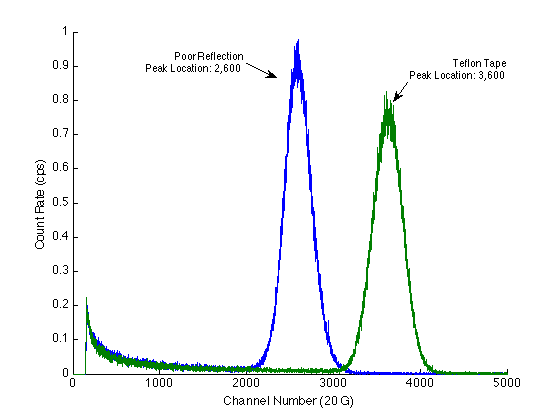
\includegraphics[width=\textwidth]{GS20_TeflonBlackTape.png}
        \end{subfigure}
        
        \begin{subfigure}[b]{\textwidth}
        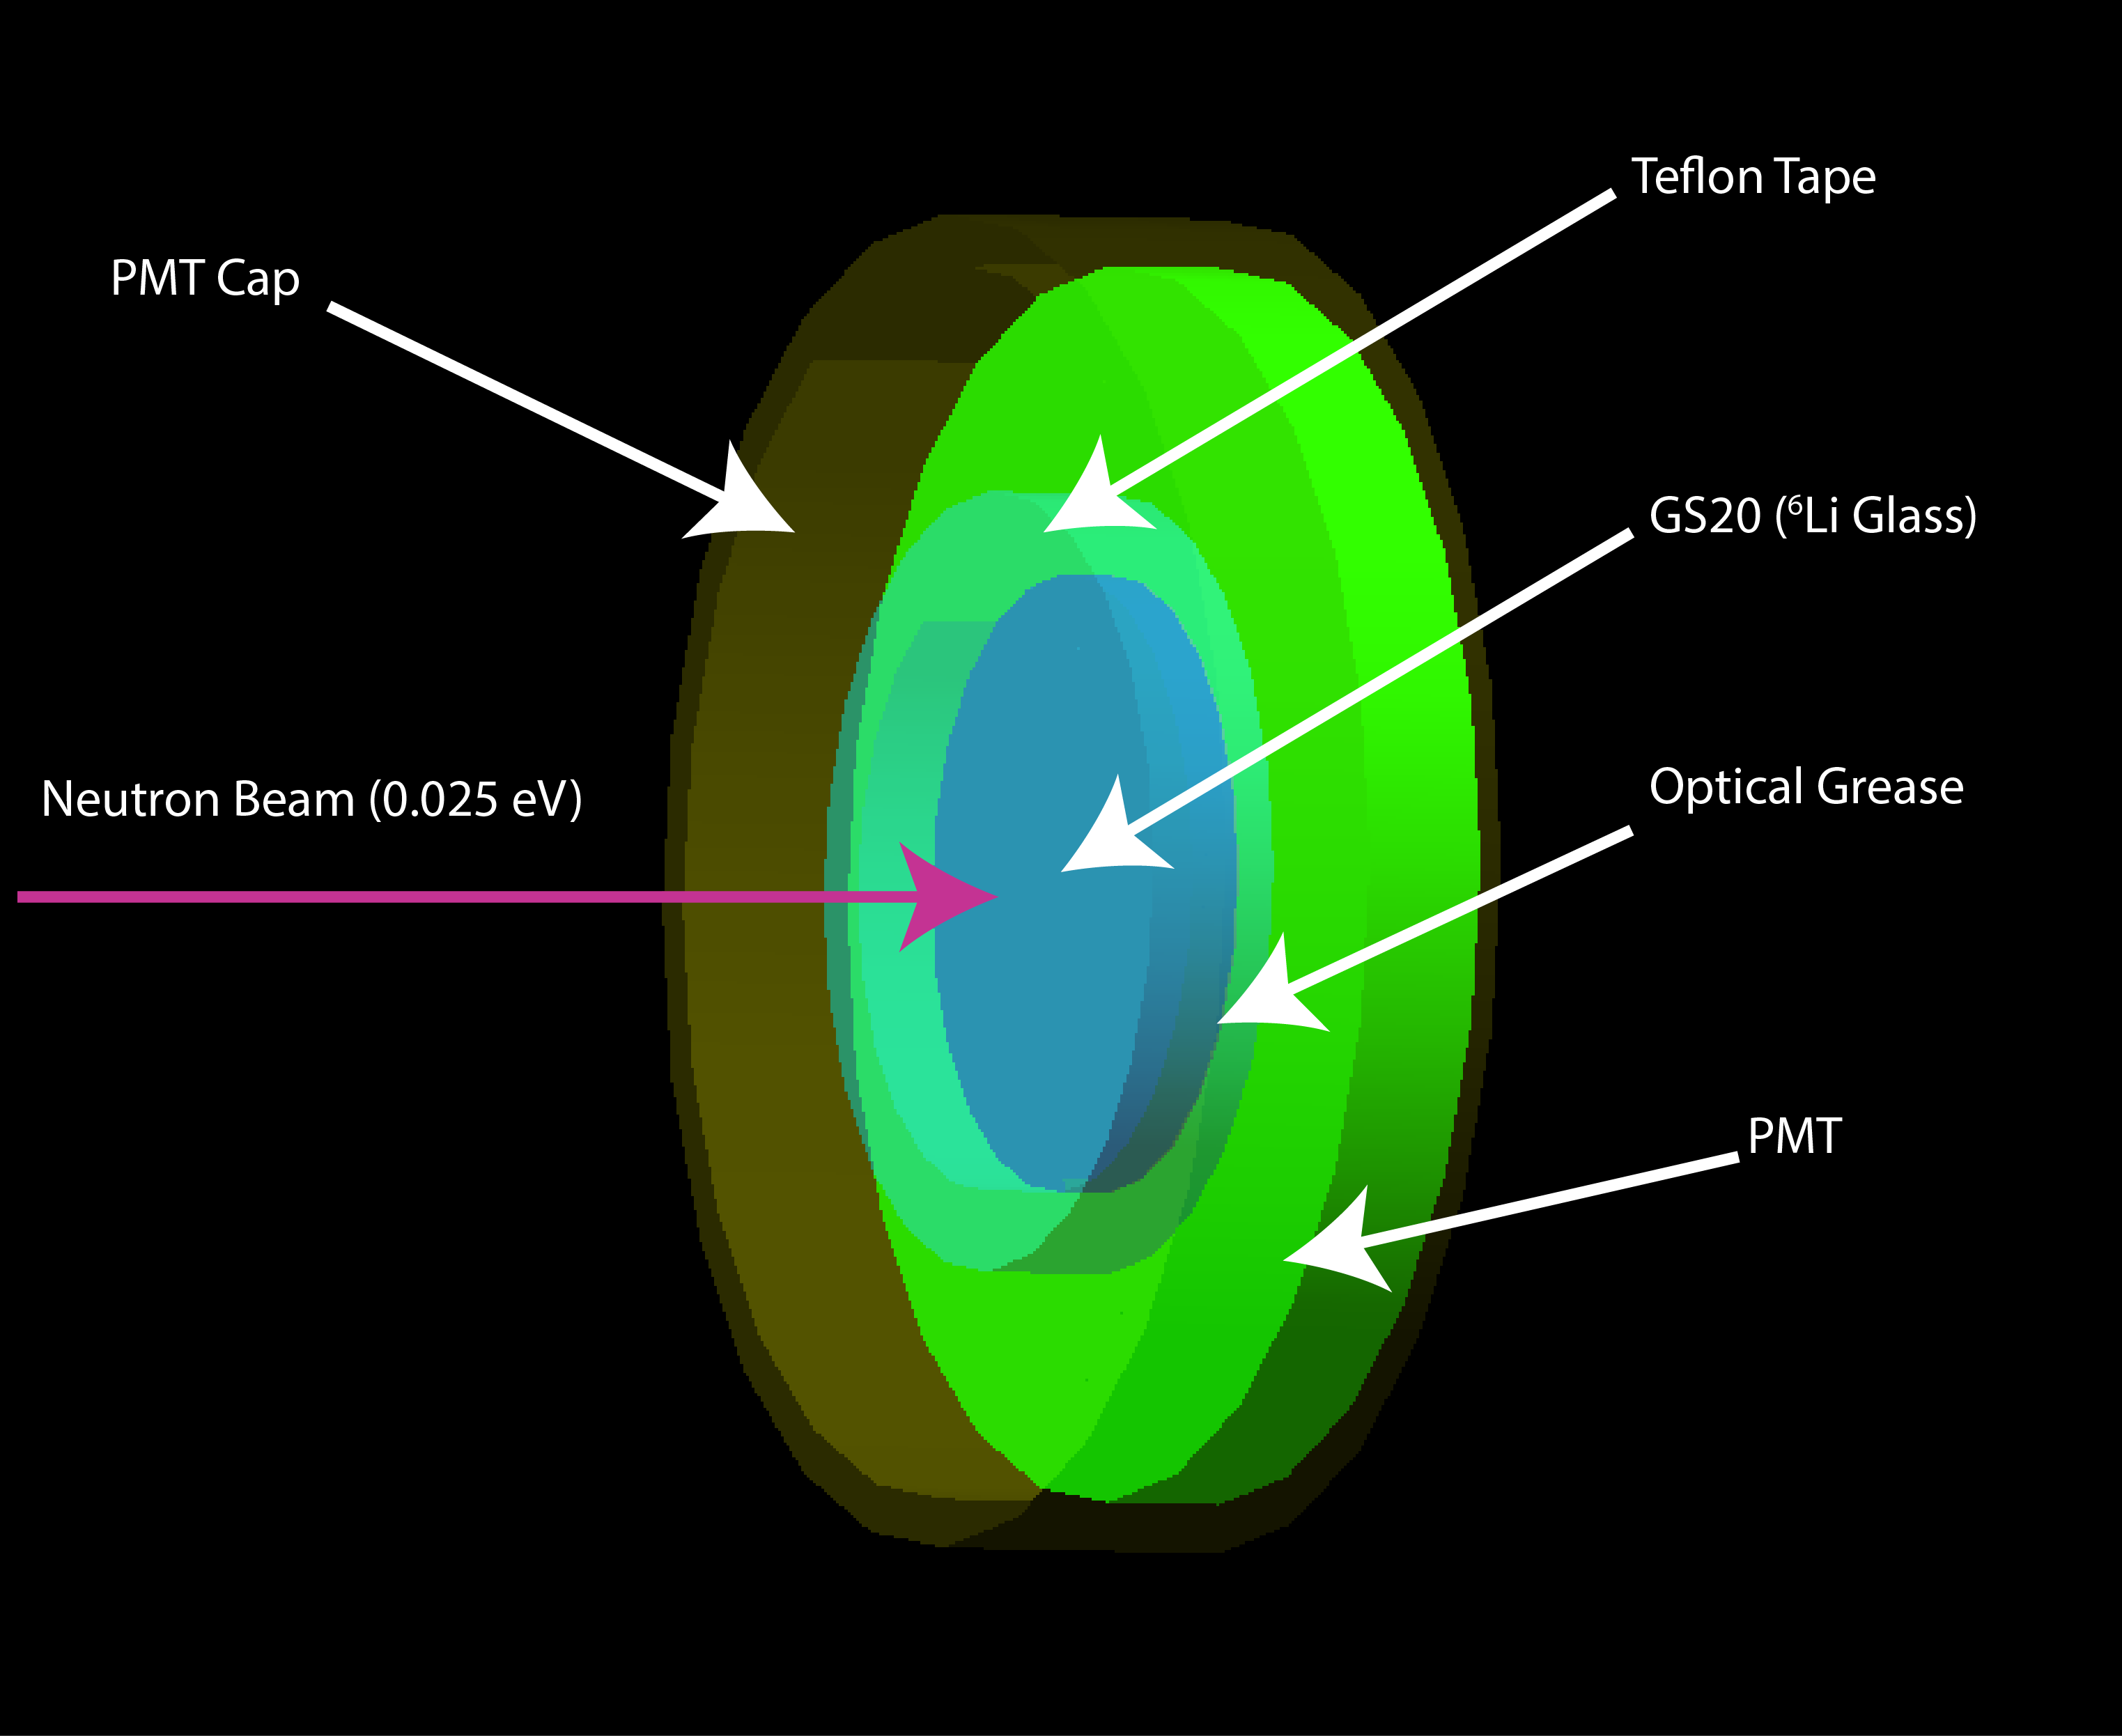
\includegraphics[width=\textwidth]{GEANT4AnnotatedGeo_GS20SimGeo.png}
        \end{subfigure}
      \end{figure}
    \end{column}
  \end{columns}
\end{frame}
%%%%%%%%%%%%%%%%%%%%%%%%%%%%%%%%%%%%%%%%%%%%%%%%%%%%%%%%%%%%%%%%%%%%%%%%%%
\begin{frame}{Small Scale Detectors}
\begin{itemize}
  \item Fabricated four 4" by 6" slab detectors
  \item Used Birks, attenuation from single film studies
  \item All values agreed within 40\%
\end{itemize}
\begin{figure}
	\centering
	\includegraphics[height=0.7\textheight]{MeasLayeredDetector_MountingLayers}
\end{figure}
\end{frame}
%%%%%%%%%%%%%%%%%%%%%%%%%%%%%%%%%%%%%%%%%%%%%%%%%%%%%%%%%%%%%%%%%%%%%%%%%%
%%%%%%%%%%%%%%%%%%%%%%%%%%%%%%%%%%%%%%%%%%%%%%%%%%%%%%%%%%%%%%%%%%%%%%%%%%
%                                                                        %
%                             RESULTS                                    %
%                                                                        %
%%%%%%%%%%%%%%%%%%%%%%%%%%%%%%%%%%%%%%%%%%%%%%%%%%%%%%%%%%%%%%%%%%%%%%%%%%
\subsection{Results}
\begin{frame}{Completed Work}
  \textbf{Neutronics, energy deposition, and light transport}
  \vspace{0.5cm}
  \begin{columns}[onlytextwidth]
    \begin{column}{0.45\textwidth}
      Geometries
      \begin{itemize}
        \item GS2O  (with and without reflector)
        \item 4 in by 6 in two layer detectors
        \item Full RPM
      \end{itemize}
    \end{column}
    \begin{column}{0.45\textwidth}
      Parameter Studies
      \begin{itemize}
        \item Light guide thickness
        \item Light guide material (WLS)
        \item Reflectivity and wrappings
      \end{itemize}
    \end{column}
  \end{columns}
\hyperlink{G4Intro}{\beamerbutton{Light Transport with GEANT4}}
\end{frame}
%%%%%%%%%%%%%%%%%%%%%%%%%%%%%%%%%%%%%%%%%%%%%%%%%%%%%%%%%%%%%%%%%%%%%%%%%%
\begin{frame}{Slab Thickness, Cladding and Light Collection Geometry}
GEANT4 simulations preformed on the slab thickness, cladding material
  \begin{figure}
    \centering
    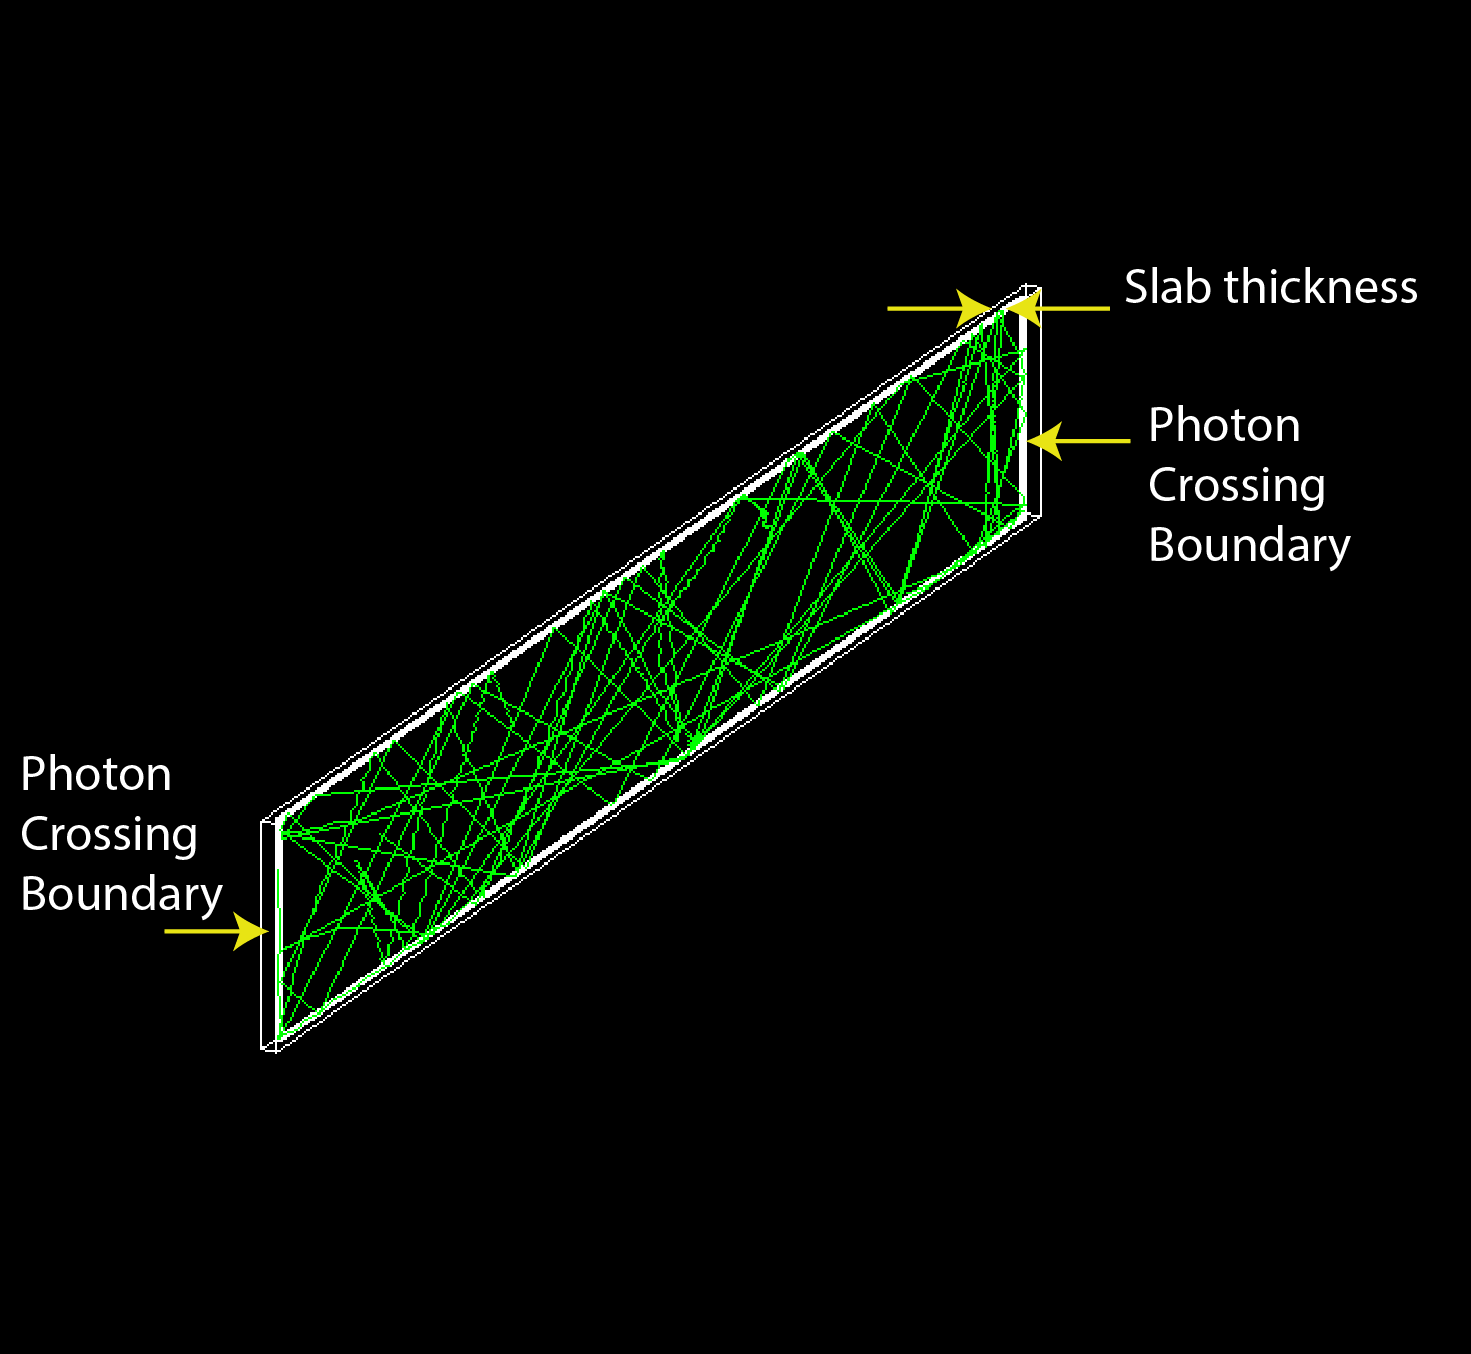
\includegraphics[height=0.7\textheight,keepaspectratio]{GEANT4AnnotatedGeo_WLSGeo}
  \end{figure}
\end{frame}
%%%%%%%%%%%%%%%%%%%%%%%%%%%%%%%%%%%%%%%%%%%%%%%%%%%%%%%%%%%%%%%%%%%%%%%%%%
\begin{frame}{Slab Thickness Effects}
Thicker slabs have better light collection
\begin{table}
	% Data for this table may be found on pg. 30 of the third lab notebook
	\small
  \begin{tabular}{c | c  c}
	\toprule
	Slab Thickness & Fraction Collected (\SI{50}{\cm}) & Fraction Collected (\SI{25}{\cm}) \\
	\midrule
	\SI{100}{\um} & 1.1\% & 1.1\% \\
	\SI{220}{\um} & 1.3\% & 1.7\% \\
	\SI{460}{\um} & 1.5\% & 1.9\% \\
	\SI{1}{\mm} & 2.2\% & 2.8\% \\
	\SI{2.2}{\mm} & 3.5\% & 4.2\% \\
	\SI{4.6}{\mm} & 5.1\% & 6.2\% \\
	\SI{1}{\cm} & 6.3\% & 7.3 \% \\
	\bottomrule
	\end{tabular}
\end{table}
\end{frame}
%%%%%%%%%%%%%%%%%%%%%%%%%%%%%%%%%%%%%%%%%%%%%%%%%%%%%%%%%%%%%%%%%%%%%%%%%%
\begin{frame}{Cladding Effects}
The material encasing the material impacts the light collection
\begin{table}
  \small
  \begin{tabular}{p{1.5cm} m{1.5cm} m{3cm} m{3cm}}
  \toprule
  & Coating & Fraction of Photons Collected & Expected Number of Photons Collected \\
  \midrule 
  \multirow{3}{*}{PS LiF} & Teflon & 4.3\% & 86\\
  				      & Air & 4.5\% & 90\\
				      & Mylar & 4.0\% & 80\\
  \midrule 
  \multirow{3}{*}{EJ-426} & Teflon & 0.46\% &736\\
  				      & Air & 0.45\% & 720\\
				      & Mylar & 0.42\% & 672 \\
 \bottomrule				 	   				  
 \end{tabular}
\end{table}
\end{frame}
%%%%%%%%%%%%%%%%%%%%%%%%%%%%%%%%%%%%%%%%%%%%%%%%%%%%%%%%%%%%%%%%%%%%%%%%%%
\begin{frame}{Simulated RPM}
  \begin{columns}[onlytextwidth]
    \begin{column}{0.45\textwidth}
		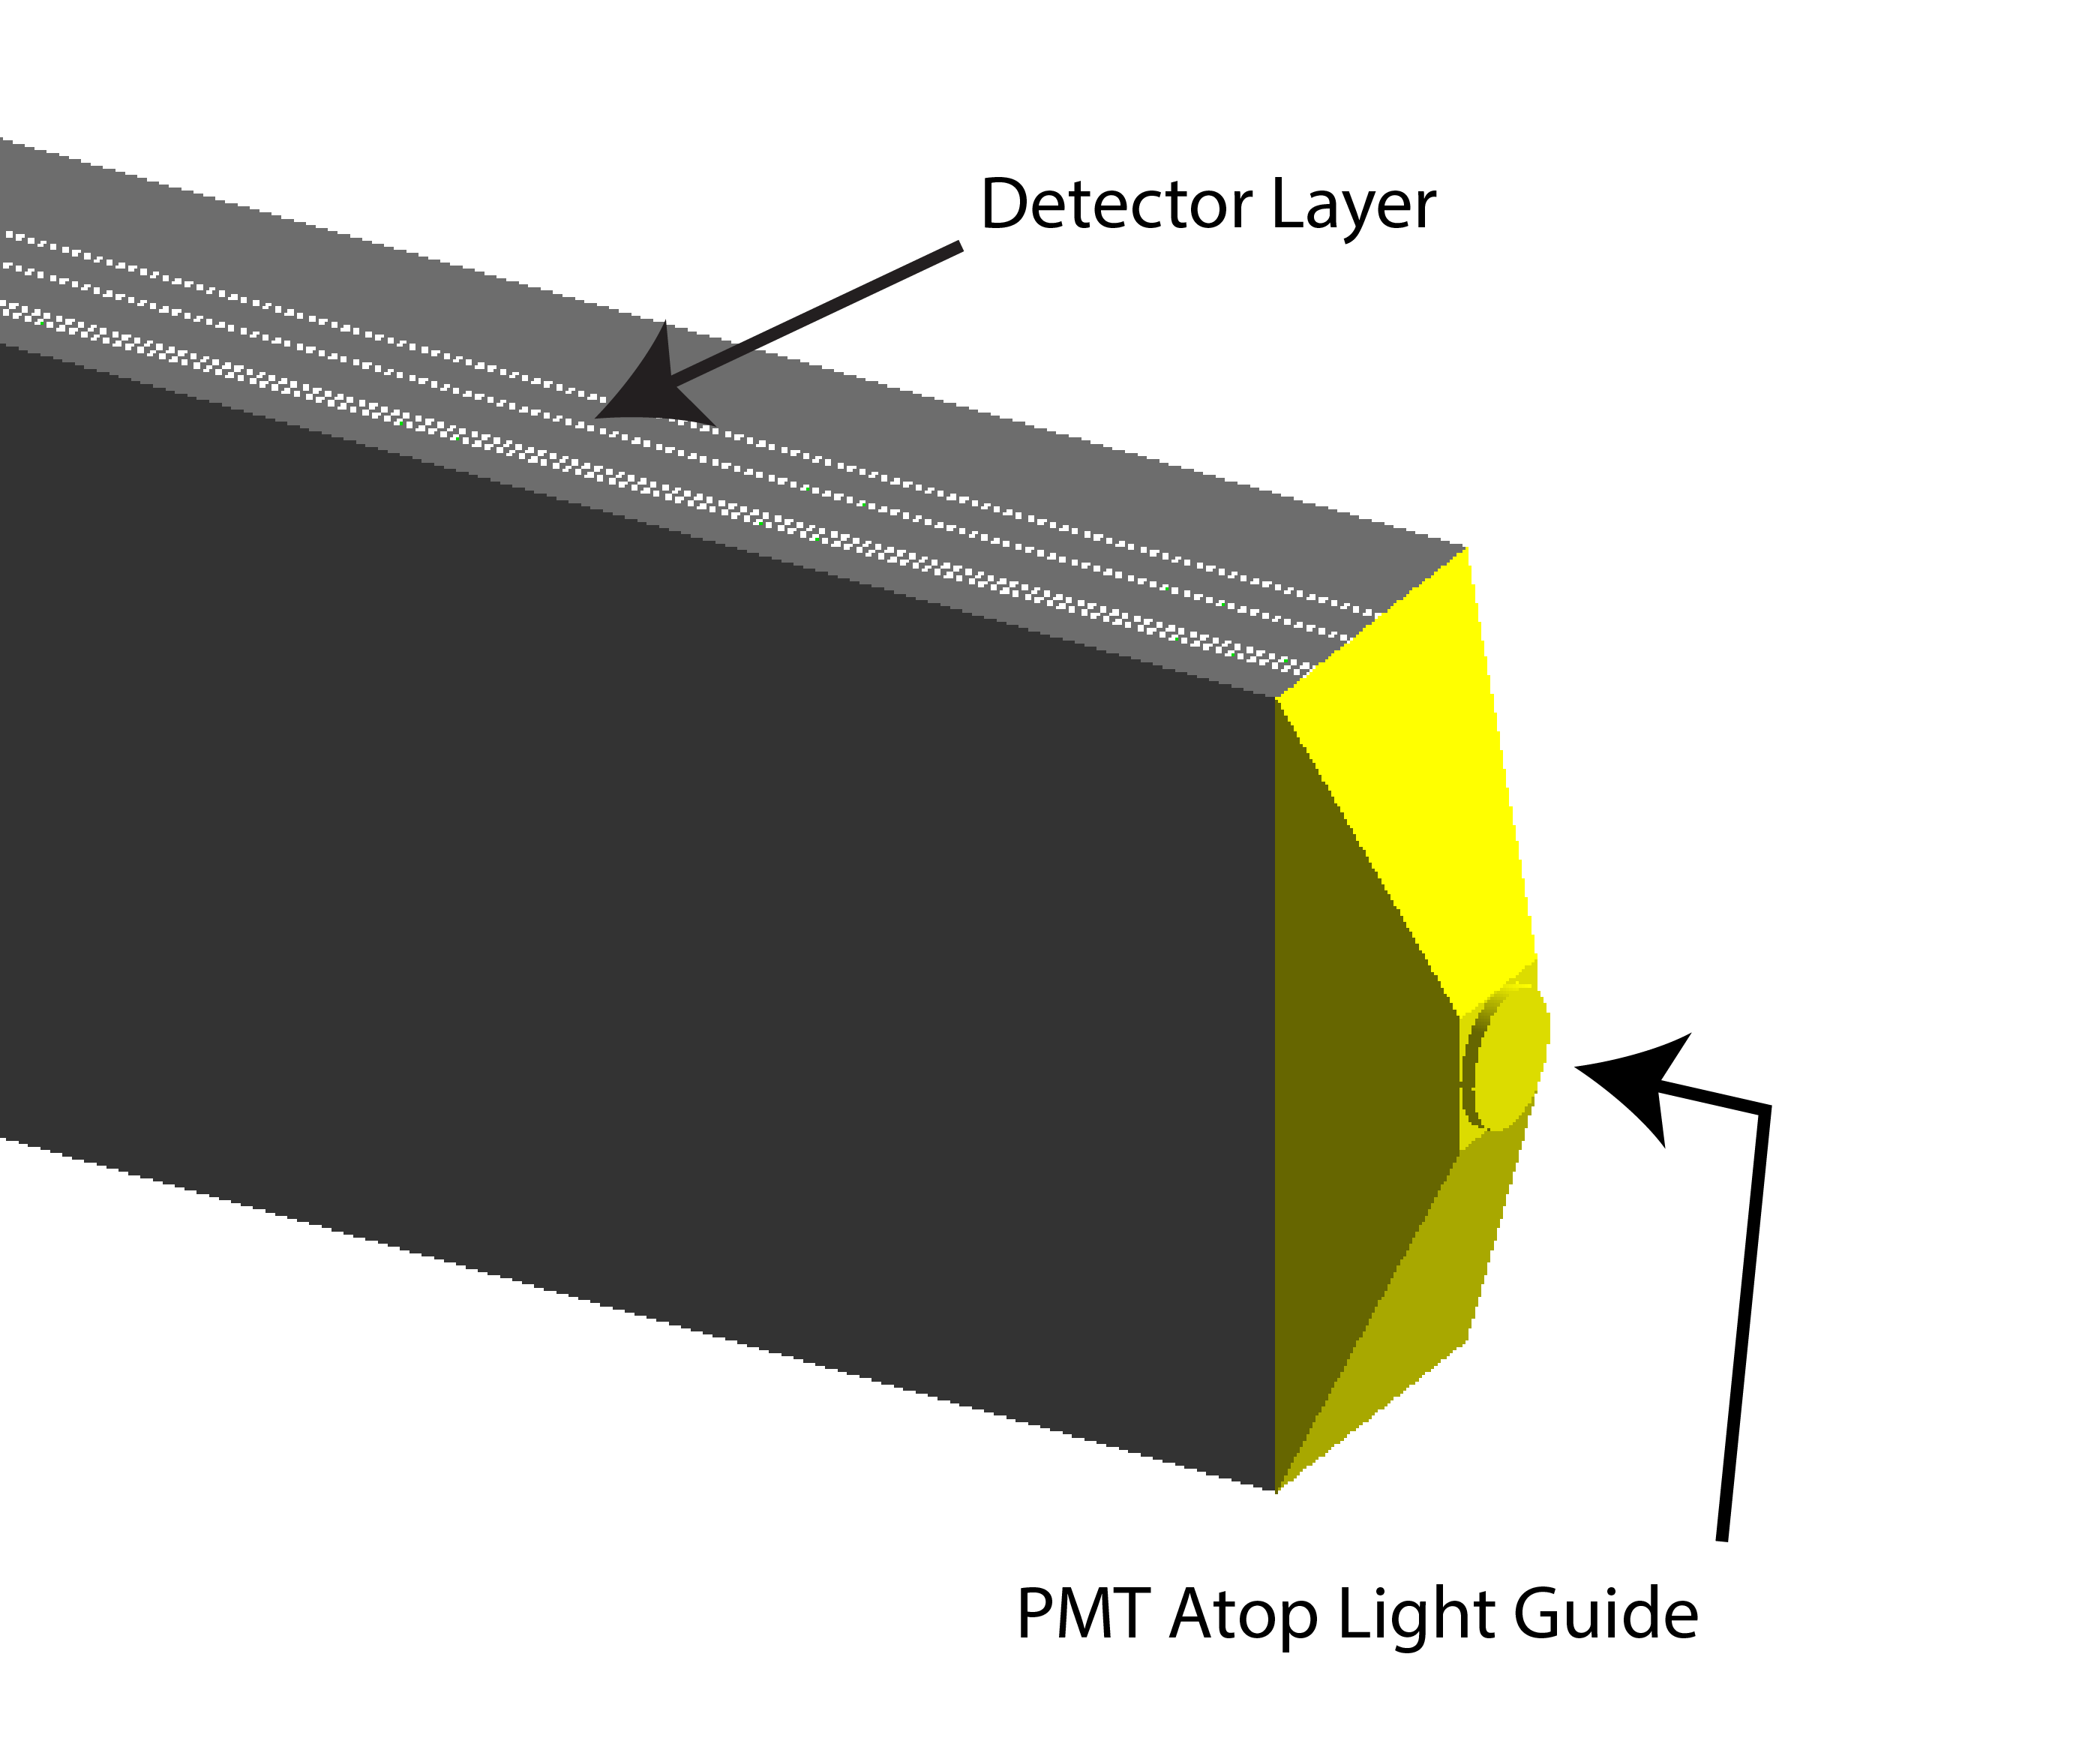
\includegraphics[width=\textwidth]{GEANT4AnnotatedGeo_RPM8SimGeoPMTEnd.png}
    \end{column}
    \begin{column}{0.45\textwidth}
		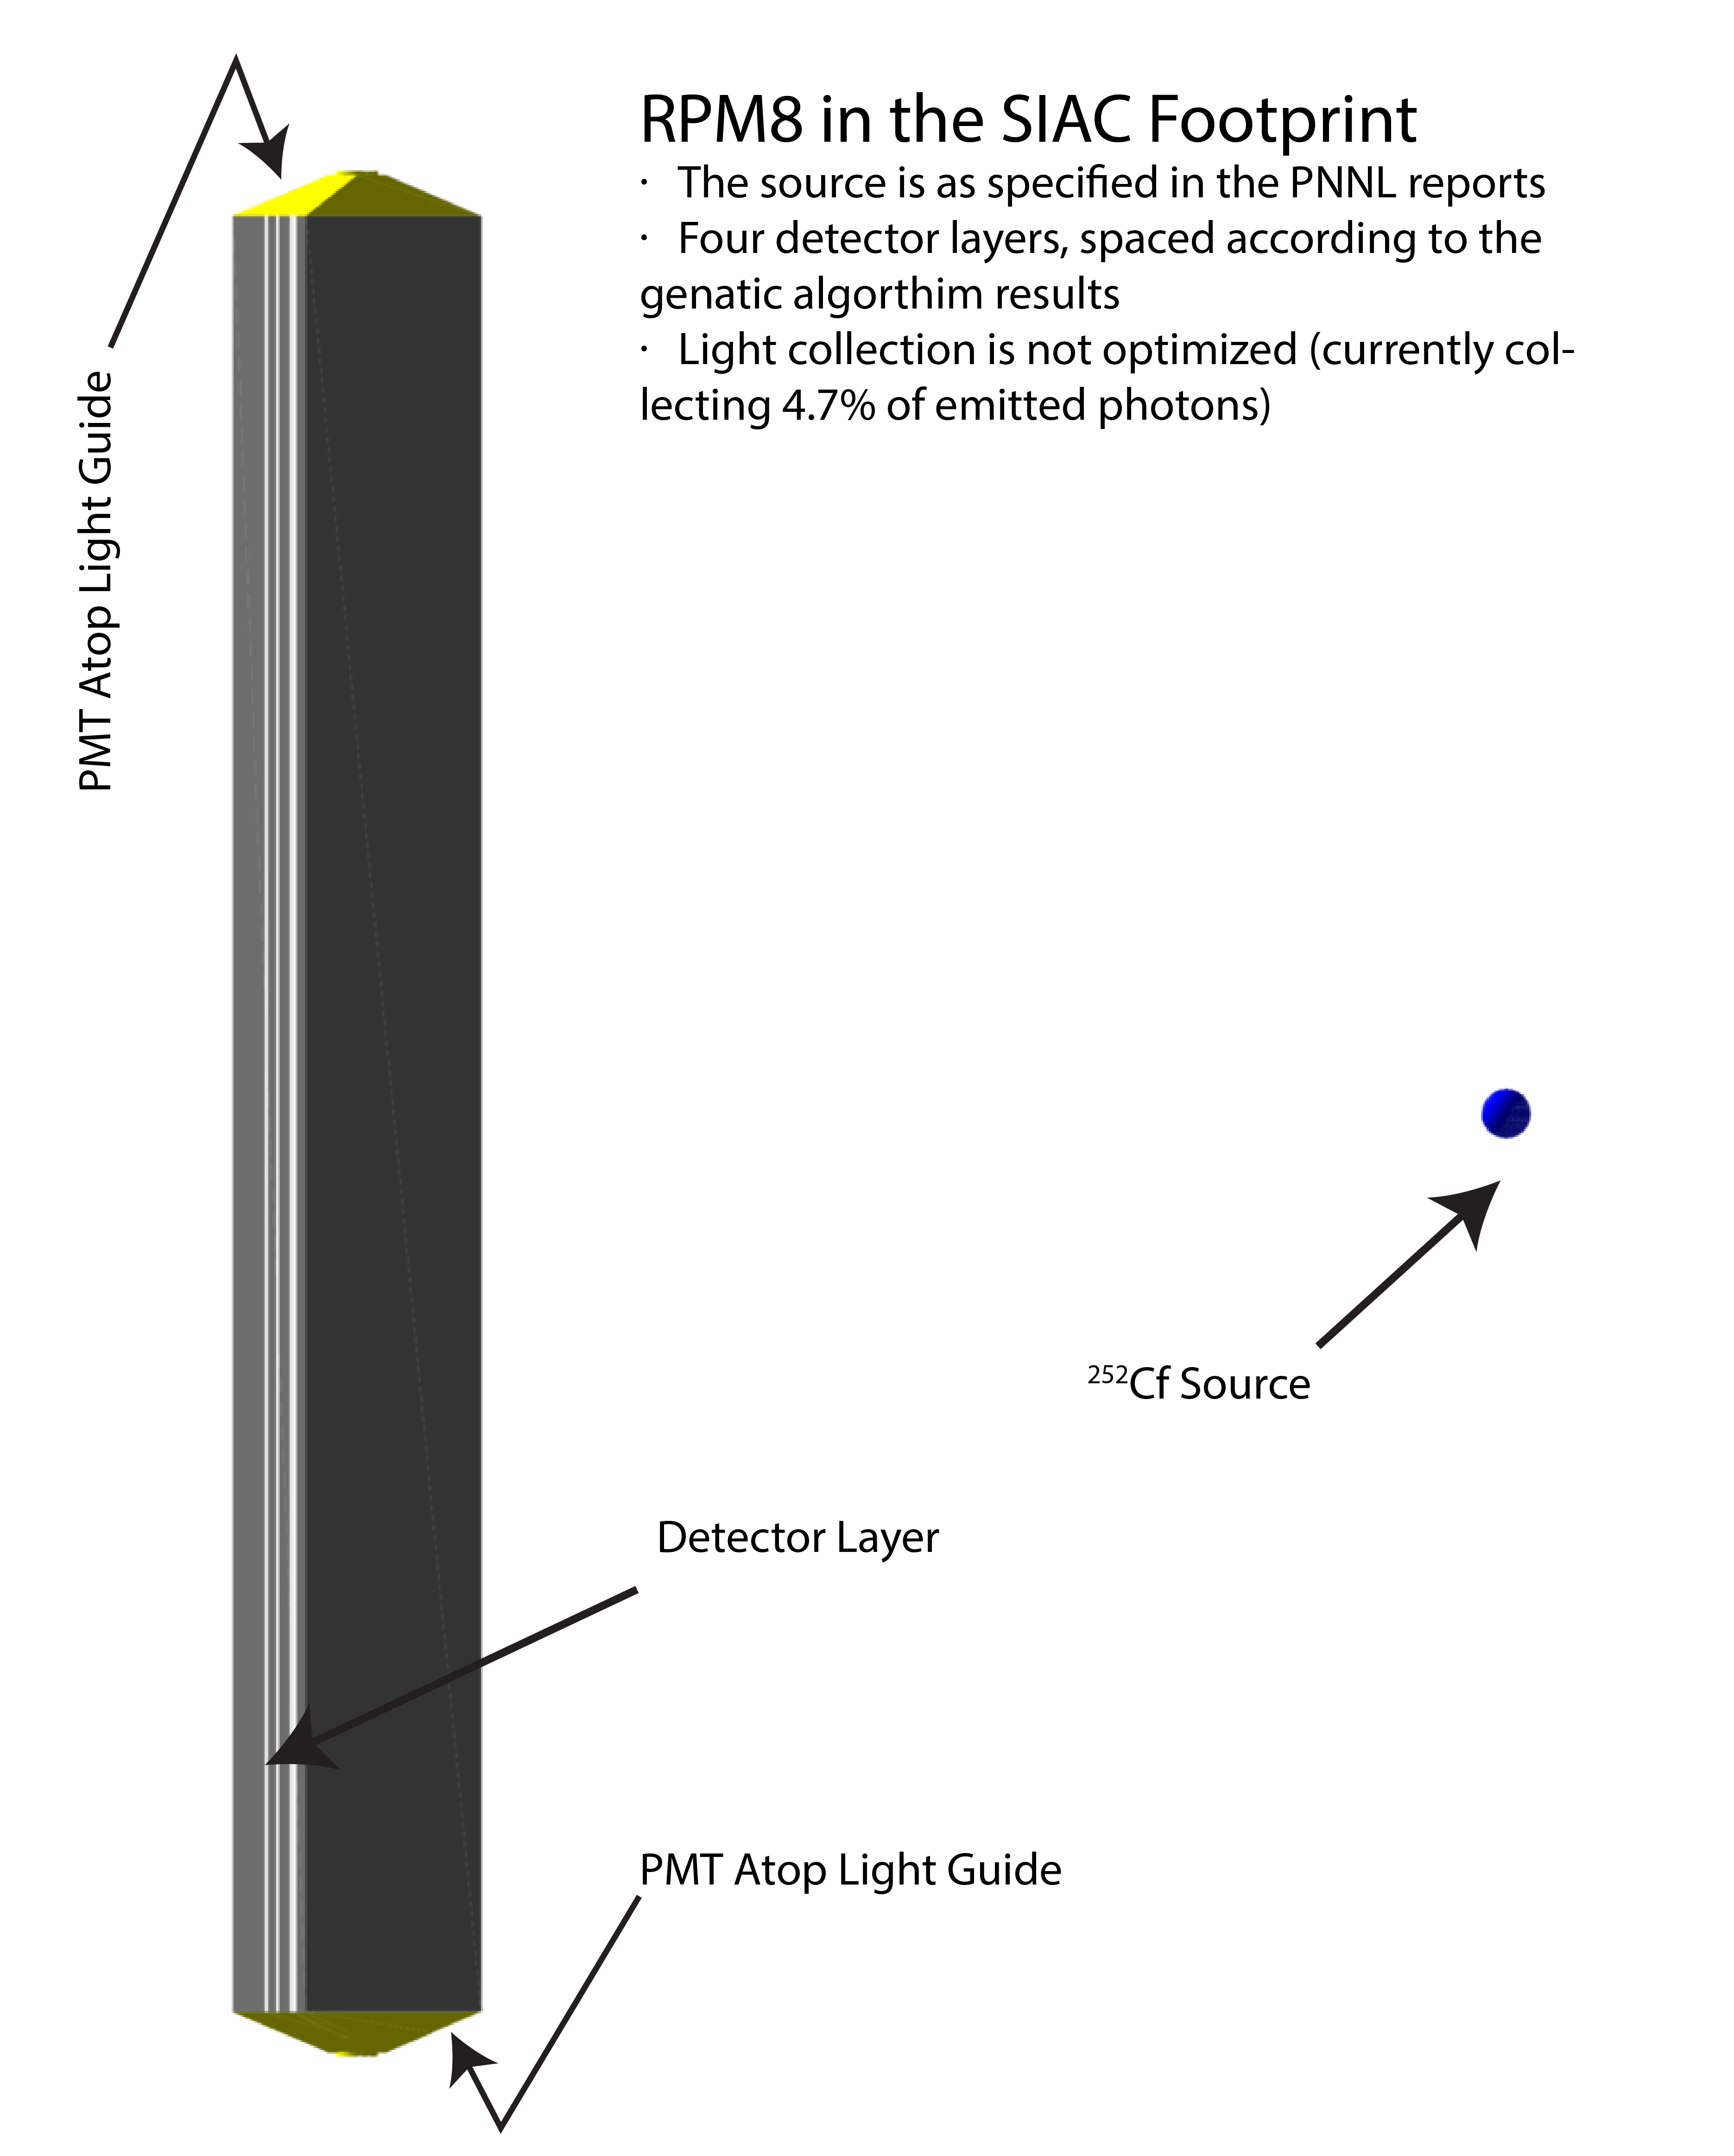
\includegraphics[width=\textwidth]{GEANT4AnnotatedGeo_RPM8SimGeo.png}
    \end{column}
  \end{columns}
\end{frame}
%%%%%%%%%%%%%%%%%%%%%%%%%%%%%%%%%%%%%%%%%%%%%%%%%%%%%%%%%%%%%%%%%%%%%%%%%%

%%%%%%%%%%%%%%%%%%%%%%%%%%%%%%%%%%%%%%%%%%%%%%%%%%%%%%%%%%%%%%%%%%%%%%%%%%
%																							                           %
%												Conclusions						                           %
%																							                           %
%%%%%%%%%%%%%%%%%%%%%%%%%%%%%%%%%%%%%%%%%%%%%%%%%%%%%%%%%%%%%%%%%%%%%%%%%%
\section{Conclusions}
\subsection*{}
%%%%%%%%%%%%%%%%%%%%%%%%%%%%%%%%%%%%%%%%%%%%%%%%%%%%%%%%%%%%%%%%%%%%%%%%%%%
\begin{frame}{Neutron - Gamma Discrimination}
  \begin{itemize}
    \item Devloped a method for pulse height discrimination to achieve a gamma intrsinic efficiency of less than \num{1E-6}
    \item Completed detailed energy simulations (and preformed validaiton)
    \item Attributed the pulse height discrimination ability to the ranges of the secondary electrons
    \item Suggested film thickness is between \SI{50}{\um} and \SI{150}{\um}
  \end{itemize}
\end{frame}
%%%%%%%%%%%%%%%%%%%%%%%%%%%%%%%%%%%%%%%%%%%%%%%%%%%%%%%%%%%%%%%%%%%%%%%%%%%
\begin{frame}{Designed Layered RPM Detector}
  \begin{itemize}
    \item Simulated layered detector designs with XSDRN, MCNPX, GEANT4
    \item Optimized a layered detector design capable of meeting the criteria
    \item Cylindrical designs show promise as well
  \end{itemize}
\end{frame}
%%%%%%%%%%%%%%%%%%%%%%%%%%%%%%%%%%%%%%%%%%%%%%%%%%%%%%%%%%%%%%%%%%%%%%%%%%%
\begin{frame}{Light Collection in an RPM}
  \begin{itemize}
    \item Completed light transport simulations of single films, 4" by 6" detector assembly, and a full scale RPM
    \item Parameter studies indicate that teflon tape is better than mylar
    \item Wavelength shifters greatly improve the light collection efficiencies
    \item Typical events in an scintillator RPM will collect between 5\% and 10\% of the emitted light
  \end{itemize}
\end{frame}
%%%%%%%%%%%%%%%%%%%%%%%%%%%%%%%%%%%%%%%%%%%%%%%%%%%%%%%%%%%%%%%%%%%%%%%%%%%
\begin{frame}{}
  \centering
  \begin{figure}
    
\includegraphics[height=3cm]{PowerTQuestion.png}
  \end{figure}
  Thanks to everyone for listening and their contributions
\end{frame}
%%%%%%%%%%%%%%%%%%%%%%%%%%%%%%%%%%%%%%%%%%%%%%%%%%%%%%%%%%%%%%%%%%%%%%%%%%%
% BILBIOLGRAPHY
%%%%%%%%%%%%%%%%%%%%%%%%%%%%%%%%%%%%%%%%%%%%%%%%%%%%%%%%%%%%%%%%%%%%%%%%%%%
\begin{frame}[plain,allowframebreaks]
\frametitle{Works Cited}
	\tiny
    \bibliography{Bib} % Bib.bib included in the references directory
\end{frame}
%%%%%%%%%%%%%%%%%%%%%%%%%%%%%%%%%%%%%%%%%%%%%%%%%%%%%%%%%%%%%%%%%%%%%%%%%%%
% BACKUP 
%%%%%%%%%%%%%%%%%%%%%%%%%%%%%%%%%%%%%%%%%%%%%%%%%%%%%%%%%%%%%%%%%%%%%%%%%%%
\appendix
\section*{Detailed Detector Requirements}
\label{PNNLCriteria}
%%%%%%%%%%%%%%%%%%%%%%%%%%%%%%%%%%%%%%%%%%%%%%%%%%%%%%%%%%%%%%%%%%%%%%%%%%%%%%%
%%%%%%%%%%%%%%%%%%%%%%%%%%%%%%%%%%%%%%%%%%%%%%%%%%%%%%%%%%%%%%%%%%%%%%%%%%%%%%%
\begin{frame}{Absolute Neutron Efficiency}
\newtheorem{pnnlTHM1}{Absolute Neutron Efficiency}
\begin{pnnlTHM1}<1->
$$\epsilon_{abs} = \frac{\text{Counts}}{\text{Quanta Radiation Emitted}}\; \; \protect \cite{knoll_radiation_2009} $$
Constraint:
$$\epsilon_{abs} \geq 2.5\; \text{cps per ng}\; {}^{252}\text{Cf}$$
\end{pnnlTHM1}
Test configuration is defined to be 1 ng ${}^{252}$Cf surrounded by 0.5 cm of lead and 2.5 cm of HDPE, with the detector midpoint 2 m from the source \cite{kouzes_alternative_2010}
\hyperlink{DHSCriteria}{\beamerbutton{Return to Detector Criteria}}
\hyperlink{toc}{\beamerbutton{Table of Contents}}
\end{frame}

%%%%%%%%%%%%%%%%%%%%%%%%%%%%%%%%%%%%%%%%%%%%%%%%%%%%%%%%%%%%%%%%%%%%%%%%%%%%%%%
\begin{frame}{Intrinsic Gamma-Neutron Detection Efficiency}
\newtheorem{pnnlTHM2}{Intrinsic Gamma-Neutron Detection Efficiency}
\begin{pnnlTHM2}<1->
$$\epsilon_{int,\gamma n} = \frac{\text{Counts}}{\text{Quanta Radiation Crossing Detector}} \; \protect \cite{kouzes_alternative_2010} $$
Constraint:
$$ \epsilon_{int,\gamma n} \leq 10^{-6} $$
\end{pnnlTHM2}
\begin{itemize}
	\item Counts over quanta crossing the detector
	\item Measured from a source that produces a 10 mR/hr field
\end{itemize}
\hyperlink{DHSCriteria}{\beamerbutton{Return to Detector Criteria}}
\hyperlink{toc}{\beamerbutton{Table of Contents}}
\end{frame}

%%%%%%%%%%%%%%%%%%%%%%%%%%%%%%%%%%%%%%%%%%%%%%%%%%%%%%%%%%%%%%%%%%%%%%%%%%%%%%%
\begin{frame}[fragile]{Gamma Absolute Rejection Ratio}
\newtheorem{pnnlTHM3}{GARRn}
\begin{pnnlTHM3}<1->
$$ GARRn = \frac{\epsilon_{abs,\gamma n}}{\epsilon_{abs,n}} \; \protect \cite{kouzes_alternative_2010} $$
Constraint:
$$ 0.9 \leq GARRn \leq 1.1 $$
\end{pnnlTHM3}
The detector's performance should change by no more than 10\% in a strong gamma field
\begin{itemize}
	\item GARRn is measured by exposing the detector to a 10 mR/hr gamma field while exposed to neutron source
	\item Count rate is measured when the gamma source is no longer present
	\item Difference determines the GARRn
\end{itemize}
\hyperlink{DHSCriteria}{\beamerbutton{Return to Detector Criteria}}
\hyperlink{toc}{\beamerbutton{Table of Contents}}
\end{frame}

\section*{Spectra and MLLD Techniques}
\label{MeasMethods}
%%%%%%%%%%%%%%%%%%%%%%%%%%%%%%%%%%%%%%%%%%%%%%%%%%%%%%%%%%%%%%%%%%%%%%%%%%%%%%%
%                                                                             %
%                                   FACILITIES                                %
%                                                                             %
%%%%%%%%%%%%%%%%%%%%%%%%%%%%%%%%%%%%%%%%%%%%%%%%%%%%%%%%%%%%%%%%%%%%%%%%%%%%%%%

%%%%%%%%%%%%%%%%%%%%%%%%%%%%%%%%%%%%%%%%%%%%%%%%%%%%%%%%%%%%%%%%%%%%%%%%%%%%%%%
\begin{frame}{Button Sources}
	\centering
	Alpha Sources
	\begin{table}[h]
		\tiny
		\begin{tabular}{c | c c}
		Source & Half-Life & Energy (MeV) \\
		\hline
		\hline
		${}^{232}$Th & $1.4\times10^{10}$ yr & 4.012 \\
		${}^{240}$Pu & $6.5\times10^{3}$ yr & 5.17 (76\%) 5.12 (24\%) \\
		${}^{241}$Am & 433 yr & 5.48 (85\%) 5.44 (12\%) \\
		${}^{239}$Pu, ${}^{241}$Am, ${}^{244}$Cm  & various & various \\
		\end{tabular}
	\end{table}
	Beta Sources
	\begin{table}[h]
		\tiny
		\begin{tabular}{c | c c}
		Source & Half-Life & Endpoint Energy (MeV)\\
		\hline
		\hline
		${}^{14}$C &  5,730 yr & 0.156 \\
		${}^{36}$Cl & $3.08\times10^{5}$ yr & 0.714 \\
		${}^{36}$Ni &  92 yr & 0.067 \\
		${}^{99}$Tc & $2.12\times10^{5}$ yr & 0.292 \\
		\end{tabular}
	\end{table}
\hyperlink{PHDMain}{\beamerbutton{Return to MLLD}}
\hyperlink{toc}{\beamerbutton{Table of Contents}}
\end{frame}

%%%%%%%%%%%%%%%%%%%%%%%%%%%%%%%%%%%%%%%%%%%%%%%%%%%%%%%%%%%%%%%%%%%%%%%%%%%%%%%
\begin{frame}{Gamma Irridiator}
\begin{columns}[onlytextwidth]
\begin{column}{0.45\textwidth}
	\begin{itemize}
		\item Desire a 10 mR/hr Gamma Field
		\item Solution is a 100 $\mu$Ci ${}^{60}$Co source
		\item Shielded by lead
	\end{itemize}
\end{column}
\begin{column}{0.45\textwidth}
	\centering
	\begin{figure}
		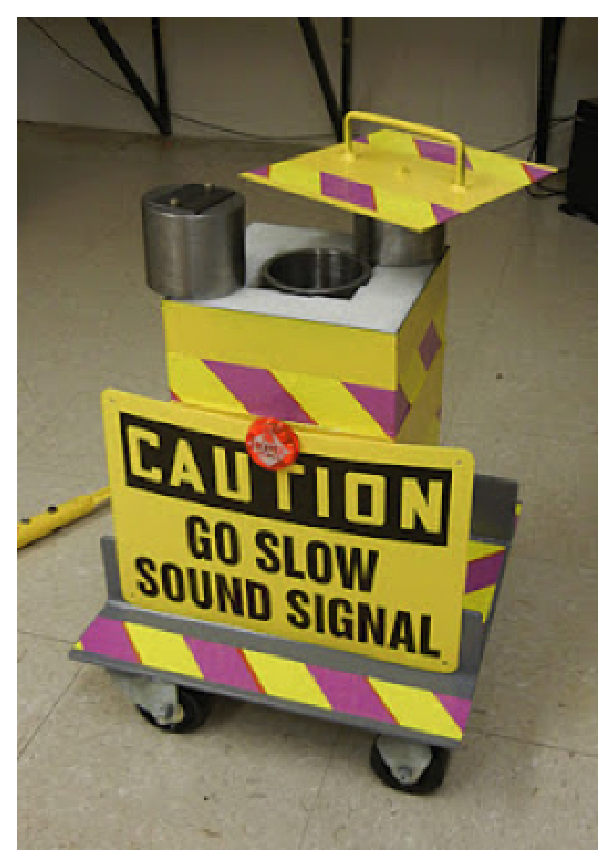
\includegraphics[width=0.8\textwidth]{GammaIrridiator.eps}
		\label{fig:GammaIrridiator}
		\caption{Gamma Irridiator}
	\end{figure}
\end{column}
\end{columns}
\hyperlink{PHDMain}{\beamerbutton{Return to MLLD}}
\hyperlink{toc}{\beamerbutton{Table of Contents}}
\end{frame}

%%%%%%%%%%%%%%%%%%%%%%%%%%%%%%%%%%%%%%%%%%%%%%%%%%%%%%%%%%%%%%%%%%%%%%%%%%%%%%%
\begin{frame}{Neutron Irridiator}
\begin{columns}[onlytextwidth]
\begin{column}{0.45\textwidth}
	\small
	\begin{itemize}
		\item Source is 0.59 $\mu$g ${}^{252}$Cf
		\item Encased in HDPE Box
		\item Two detector wells
		\begin{itemize}
			\tiny
			\item Lead Well
			\item Cadmium Well
		\end{itemize}
	\end{itemize}
\end{column}
\begin{column}{0.45\textwidth}
	\begin{figure}
		\centering
		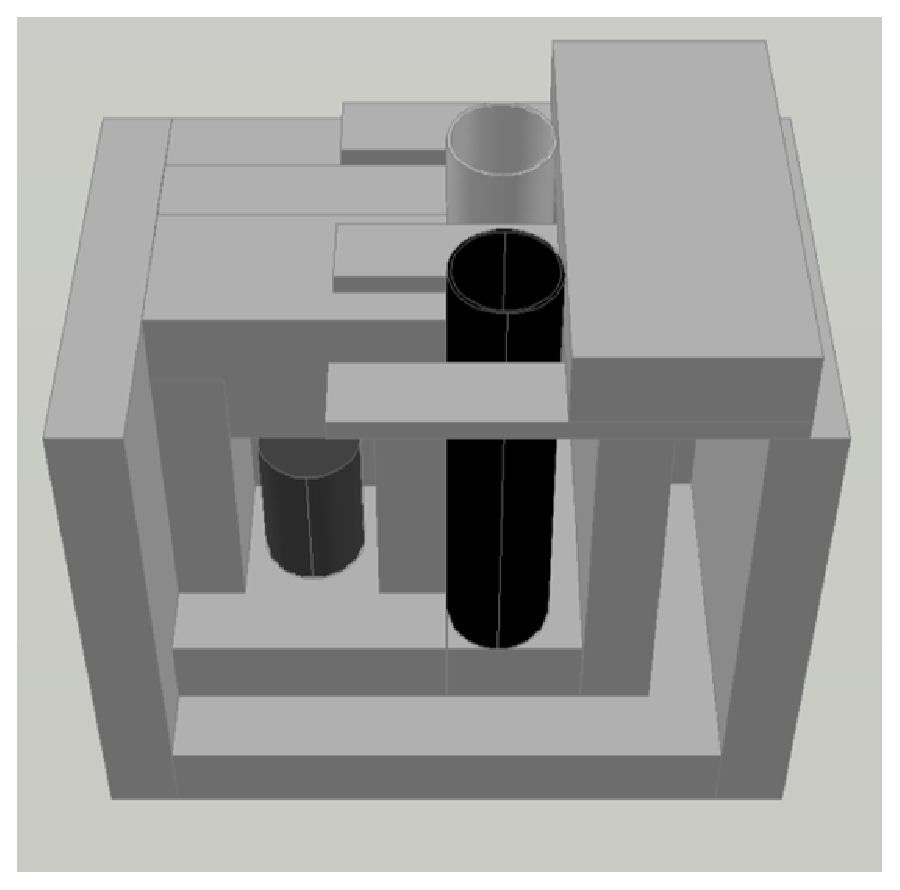
\includegraphics[height=0.25\textheight]{NeutronIrridiator_CAD.eps}
		\caption{CAD Rendering of Neutron Irridiator}
		\label{fig:NeutronIrridiatorCAD}
		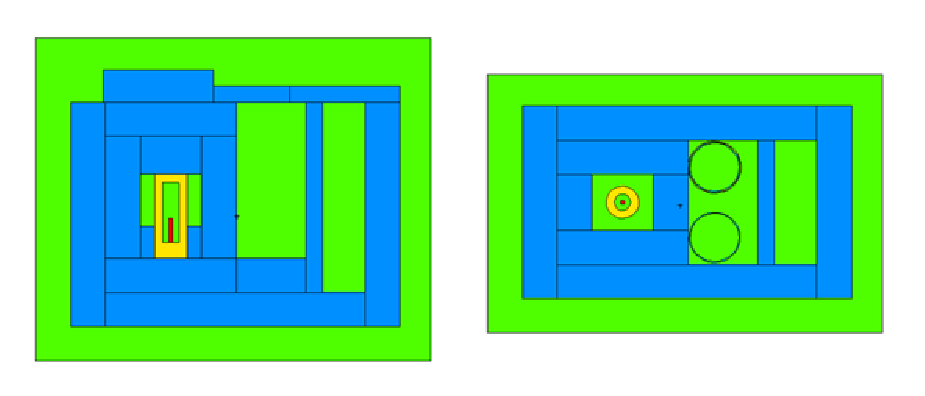
\includegraphics[height=0.25\textheight]{NeutronIrridiator_MCNP.eps}
		\caption{MCNPX Rendering of Neutron Irridiator}
		\label{fig:NeutronIrridiatorMNCPX}
	\end{figure}
\end{column}
\end{columns}
\hyperlink{PHDMain}{\beamerbutton{Return to MLLD}}
\hyperlink{toc}{\beamerbutton{Table of Contents}}
\end{frame}

%%%%%%%%%%%%%%%%%%%%%%%%%%%%%%%%%%%%%%%%%%%%%%%%%%%%%%%%%%%%%%%%%%%%%%%%%%%%%%%
\begin{frame}{Neutron Irridiator (Spectra)}
\begin{columns}[onlytextwidth]
\begin{column}{0.45\textwidth}
	\begin{itemize}
		\small
		\item Lead Well
		\begin{itemize}
			\tiny
			\item Neutrons of all energies
			\item Lead to match photon attenuation of cadmium
		\end{itemize}
		\small
		\item Cadmium Well
		\begin{itemize}
			\tiny
			\item Cadmium cutoff is about 0.5 eV
			\item Well response is to fast neutrons
			\item Shielding of photons from cadmium
		\end{itemize}
		\small 
		\item Subtraction is preformed between the two response to extract the response from thermal neutrons
	\end{itemize}
\end{column}
\begin{column}{0.45\textwidth}
	\begin{figure}
		\centering
		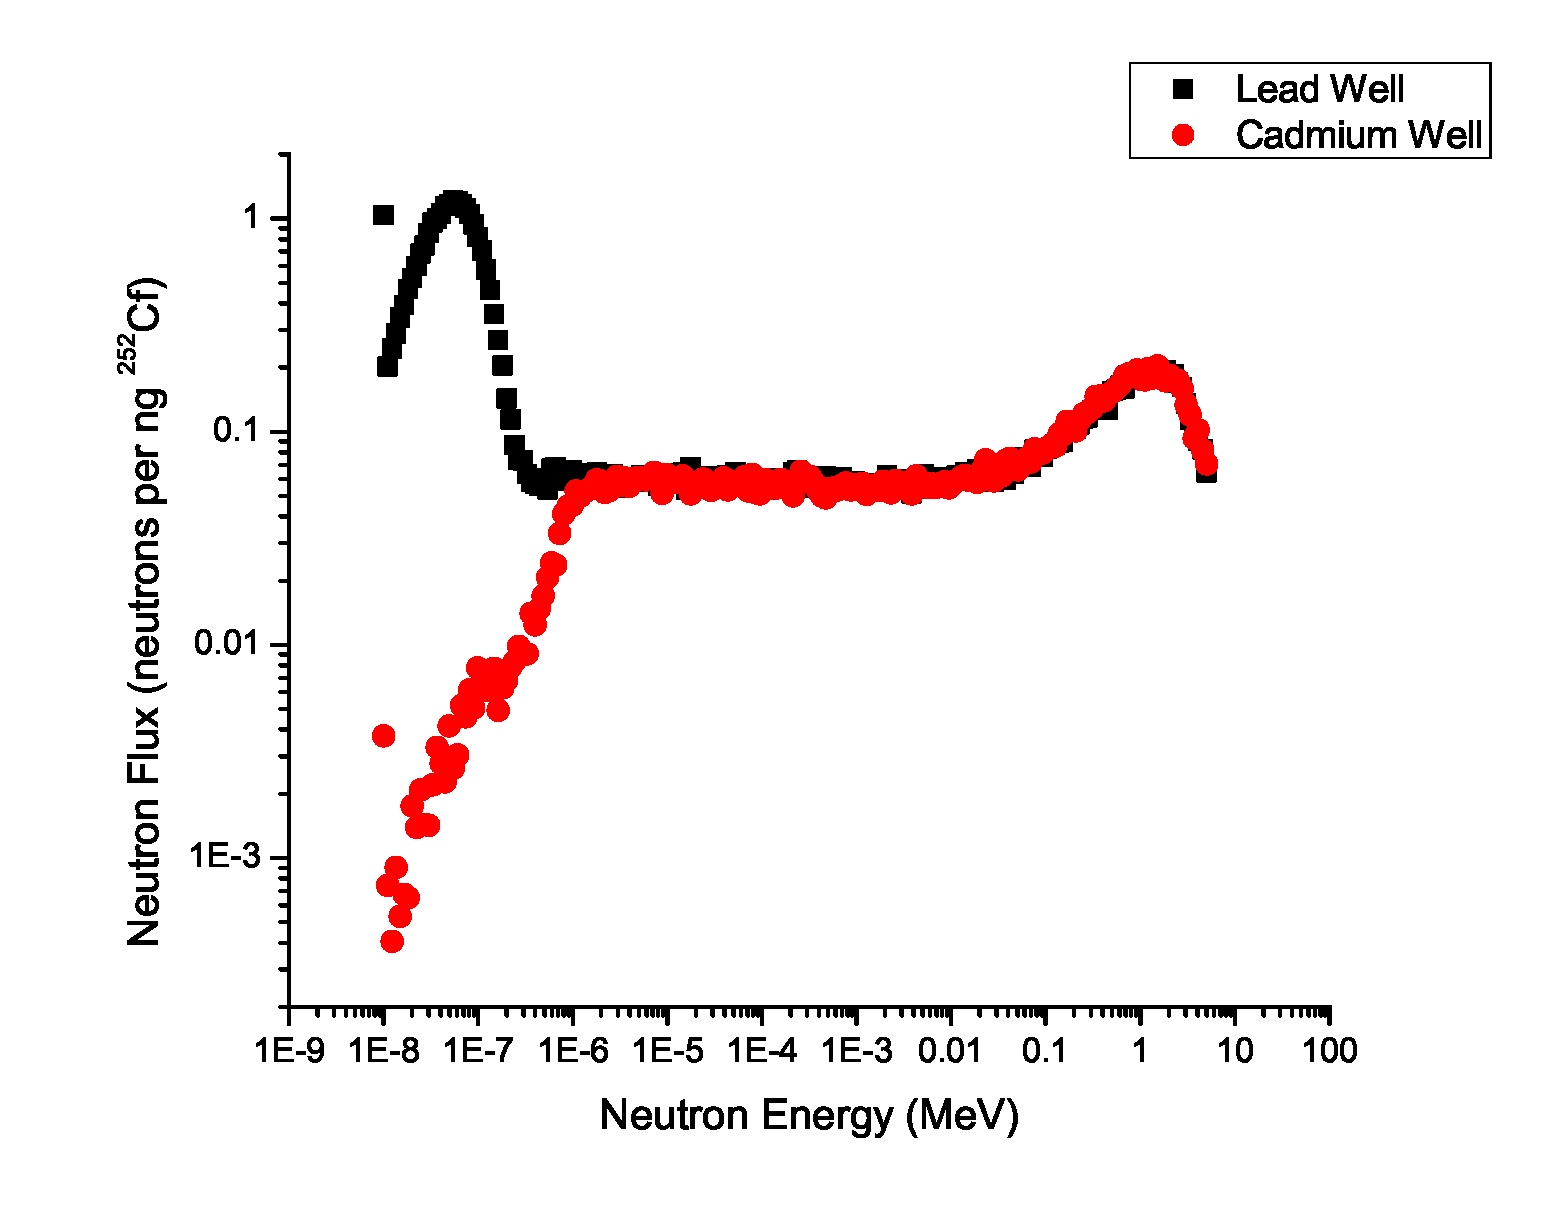
\includegraphics[width=\textwidth]{Graph19N.eps}
		\caption{Simulated Lead and Cadmium Well Spectra}
		\label{fig:SimPbCdSpectra}
	\end{figure}
\end{column}
\end{columns}
\hyperlink{PHDMain}{\beamerbutton{Return to MLLD}}
\hyperlink{toc}{\beamerbutton{Table of Contents}}
\end{frame}
%%%%%%%%%%%%%%%%%%%%%%%%%%%%%%%%%%%%%%%%%%%%%%%%%%%%%%%%%%%%%%%%%%%%%%%%%%%%%%%
\begin{frame}{Spectra Electronics}
\begin{columns}[onlytextwidth]
\begin{column}{0.45\textwidth}
	\small 
	Measurement Protocol
	\begin{itemize}
		\tiny
		\item Verify instrument gains are stable
		\begin{itemize}
			\tiny
			\item GS20 (${}^6$Li glass) is used as the standard
			\item Set voltage and coarse gain, adjust fine gain
		\end{itemize}
		\tiny
		\item Obtain a spectra from an alpha (${}^{241}$Am) 
		\item Obtain a spectra from a beta (${}^{36}$Cl)
		\item Obtain a lead well neutron spectra
		\item Obtain a cadmium well neutron spectra
		\item Obtain a gamma irridiator spectra
	\end{itemize}
\end{column}
\begin{column}{0.45\textwidth}
	\begin{figure}
		\centering
		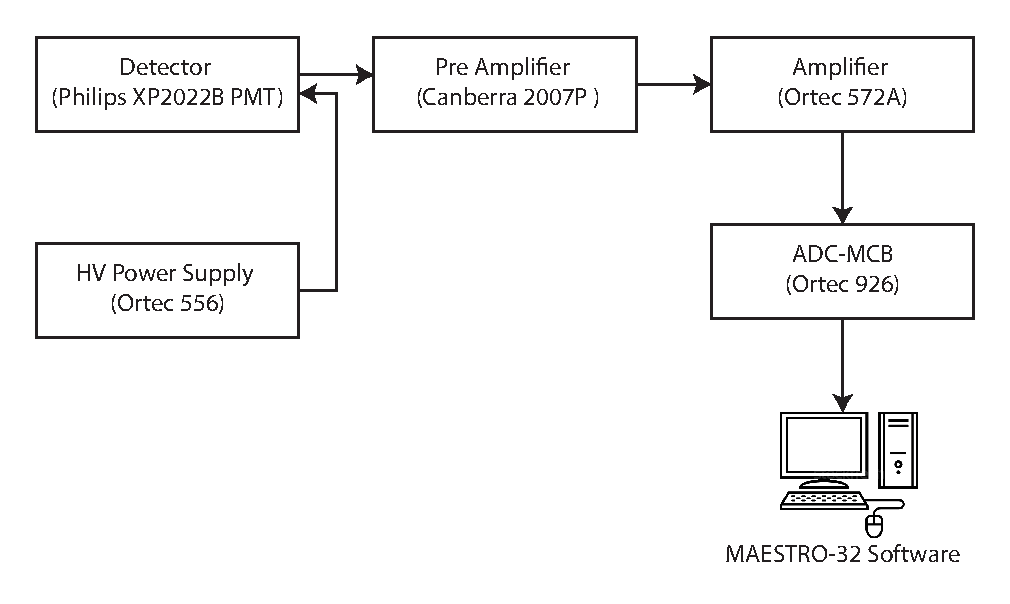
\includegraphics[height=0.5\textwidth]{ElectronicsSpectra.eps}
		\caption{Electronic Setup for Spectra}
		\label{fig:ElectronicsSpectra}
	\end{figure}
\end{column}
\end{columns}
\hyperlink{PHDMain}{\beamerbutton{Return to MLLD}}
\hyperlink{toc}{\beamerbutton{Table of Contents}}
\end{frame}
%%%%%%%%%%%%%%%%%%%%%%%%%%%%%%%%%%%%%%%%%%%%%%%%%%%%%%%%%%%%%%%%%%%%%%%%%%%%%%%
%                                                                             %
%                             ANALYSIS METHDOS                                %
%                                                                             %
%%%%%%%%%%%%%%%%%%%%%%%%%%%%%%%%%%%%%%%%%%%%%%%%%%%%%%%%%%%%%%%%%%%%%%%%%%%%%%%
\begin{frame}{Spectra Average}
	\begin{itemize}
		\item Thin films do not have clearly define features
		\item Spectra averages defined to create a feature
	\end{itemize}
\begin{columns}[onlytextwidth]
\begin{column}{0.45\textwidth}
	\newtheorem{MeasMethTHM4}{Spectra Average}
	\begin{MeasMethTHM4}<1->
		$$<\mu> = \frac{\int_{0}^{\infty}x\cdot f(x)dx}{\int_{0}^{\infty}f(x)dx} $$
		where:
		\begin{itemize}
			\tiny
			\item $<\mu>$ is the average of the spectra
			\item $f(x)$ is the spectra
			\item $x$ is a channel number
		\end{itemize}
	\end{MeasMethTHM4}
\end{column}
\begin{column}{0.45\textwidth}
	\begin{figure}
		\centering
		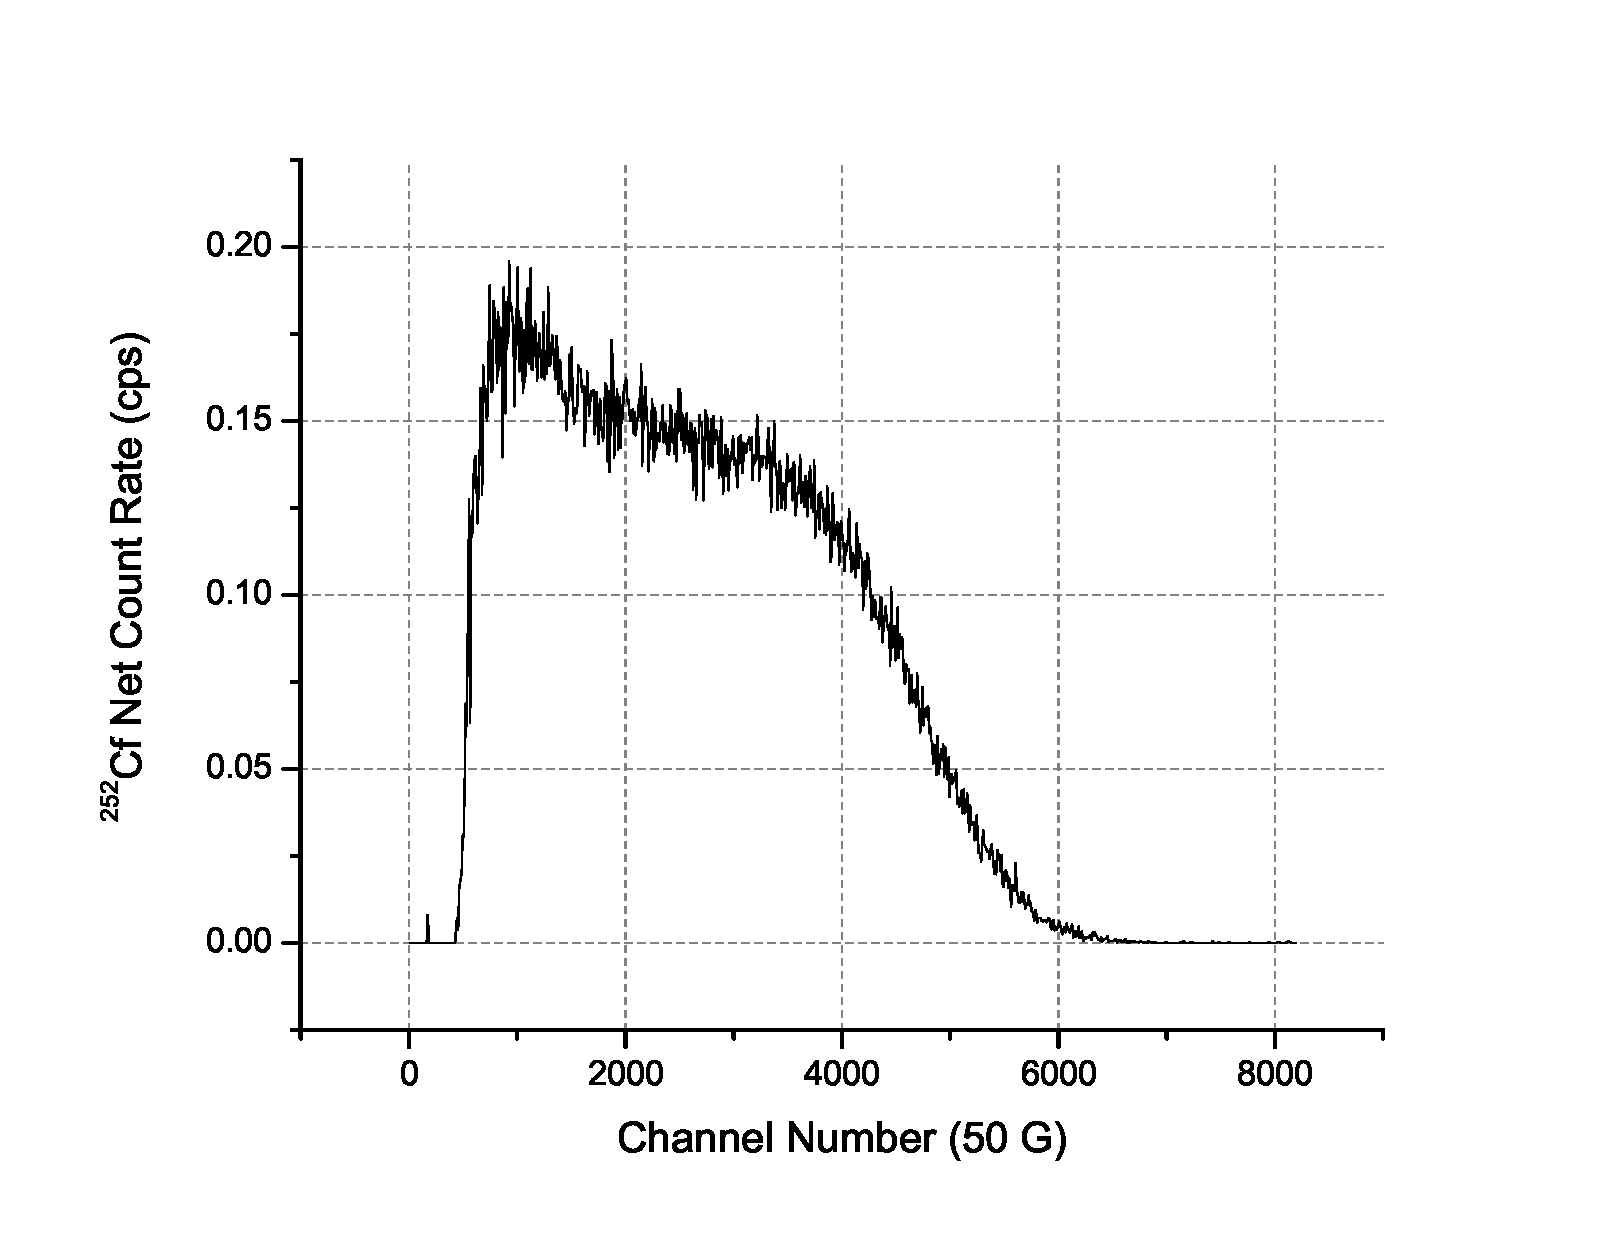
\includegraphics[width=\textwidth]{StrechedPEN-Neutron.eps}
		\caption{Example Neutron Spectra}
	\end{figure}
\end{column}
\end{columns}
\hyperlink{PHDMain}{\beamerbutton{Return to MLLD}}
\hyperlink{toc}{\beamerbutton{Table of Contents}}
\end{frame}
%%%%%%%%%%%%%%%%%%%%%%%%%%%%%%%%%%%%%%%%%%%%%%%%%%%%%%%%%%%%%%%%%%%%%%%%%%%%%%%
\begin{frame}{Pulse Height Defect}
	\newtheorem{MeasMethTHM5}{Pulse Height Defect}
	\begin{MeasMethTHM5}<1->
	\tiny
	$$ PHD_{GS20} = \frac{\dfrac{n_{peak}}{4.78\;\text{MeV}}}{\dfrac{CE_\gamma}{1.038\;\text{MeV}}} $$
		where:
		\begin{itemize}
			\tiny
			\item $PHD_{GS20}$ is the pulse height defect for GS20
			\item $n_{peak}$ is the location of the peak in the neutron spectra
			\item $CE_\gamma$ is the Compton Edge of the Gamma Spectra
		\end{itemize}
	\end{MeasMethTHM5}
	\newtheorem{MeasMethTHM6}{Pulse Height Defect (Sample)}
	\begin{MeasMethTHM6}<1->
	\tiny
	$$ PHD_{Sample} = PHD_{GS20} \frac{<n>_{sample}}{<n>_{GS20}} $$
		where:
		\begin{itemize}
			\tiny
			\item $PHD_{GS20}$ is the pulse height defect for GS20
			\item $<n>_{sample}$ is the average of the sample's neutron spectra
			\item $<n>_{GS20}$ is the average of GS20's neutron spectra
		\end{itemize}
	\end{MeasMethTHM6}
\hyperlink{PHDMain}{\beamerbutton{Return to MLLD}}
\hyperlink{toc}{\beamerbutton{Table of Contents}}
\end{frame}
%%%%%%%%%%%%%%%%%%%%%%%%%%%%%%%%%%%%%%%%%%%%%%%%%%%%%%%%%%%%%%%%%%%%%%%%%%%%%%%
\begin{frame}{Light Yield}
	\newtheorem{MeasMethTHM7}{Light Yield}
	\begin{MeasMethTHM7}<1->
	\tiny
	$$ LY_{n} = 3,800 \frac{\text{Photons}}{\text{MeV}}\frac{<n>_{sample}}{<n>_{GS20}} $$
	$$ LY_{\beta} = 3,800 \frac{\text{Photons}}{\text{MeV}}\frac{<\beta>_{sample}}{<\beta>_{GS20}} $$
	$$ LY_{\gamma} = 3,800 \frac{\text{Photons}}{\text{MeV}}\frac{<\gamma>_{sample}}{<\gamma>_{GS20}} $$
		where:
		\begin{itemize}
			\tiny
			\item $<n>_{sample}$ is the average of the sample's neutron spectra
			\item $<n>_{GS20}$ is the average of GS20's neutron spectra
			\item $<\beta>_{sample}$ is the average of the sample's beta (${}^{36}$Cl) spectra
			\item $<\beta>_{GS20}$ is the average of GS20's bet (${}^{36}$Cl) spectra
			\item $<\gamma>_{sample}$ is the average of the sample's gamma (${}^{60}$Co) spectra
			\item $<\gamma>_{GS20}$ is the average of GS20's gamma (${}^{60}$Co) spectra
		\end{itemize}
	\end{MeasMethTHM7}
\hyperlink{PHDMain}{\beamerbutton{Return to MLLD}}
\hyperlink{toc}{\beamerbutton{Table of Contents}}
\end{frame}
%%%%%%%%%%%%%%%%%%%%%%%%%%%%%%%%%%%%%%%%%%%%%%%%%%%%%%%%%%%%%%%%%%%%%%%%%%%%%%%
\begin{frame}
	\newtheorem{MeasMethTHM8}{Gamma Intrinsic Efficiency}
	\begin{MeasMethTHM8}<1->
		$$ \epsilon_{int,\gamma} = \frac{\int_{MLLD}^{\infty}{f(x)dx}}{\text{Particles Incident}} $$
	where:
	\begin{itemize}
		\tiny
		\item $MLLD$ is the mathematical lower level discriminator
		\item $f(x)$ is the spectra
		\item $\text{Particles Incident}$ is the number of incident particles
	\end{itemize}
	\end{MeasMethTHM8}
	\newtheorem{rmk1}{Mathematical Lower Level Discriminator}
	\begin{rmk1}
		\tiny
		Mathematical lower level discriminator (MLLD) is defined to be the channel at which $\epsilon_{int,\gamma} \leq 10^{-6}$
	\end{rmk1}

	\begin{itemize}
		\tiny
		\item MLLD for a film is determined from a ${}^{60}$Co measurement
		\item Source produces a 10 mR/hr field at detector surface
		\item Particles incident determined from simulation
	\end{itemize}
\hyperlink{PHDMain}{\beamerbutton{Return to MLLD}}
\hyperlink{toc}{\beamerbutton{Table of Contents}}
\end{frame}
%%%%%%%%%%%%%%%%%%%%%%%%%%%%%%%%%%%%%%%%%%%%%%%%%%%%%%%%%%%%%%%%%%%%%%%%%%%%%%%

\section*{GEANT4 Introduction}
\label{G4Intro}
\begin{frame}[fragile]{GEANT4 Introduction}
What GEANT4 is:
\begin{itemize}
  \small
  \item \href{geant4.cern.ch}{geant4.cern.ch}
  \item Free software package for the simulation of the passage of particles through matter
  \item Essentially a collection of tools for geometry, materials, physics models, events and digitization, visualizations $\dots$
  \item Maintained by the CERN community, widely used in physics
\end{itemize}
What GEANT4 is not:
\begin{itemize}
  \small
  \item For the timid
  \begin{itemize}
    \item Users are responsible for correctly implementing their own physics
    \item Users are responsible for correctly implementing their own analysis
  \end{itemize}
  \item Stagnant - major release are still occurring
\end{itemize}
\hyperlink{G4Main}{\beamerbutton{Return to Energy Deposition}}
\hyperlink{toc}{\beamerbutton{Table of Contents}}
\end{frame}
%%%%%%%%%%%%%%%%%%%%%%%%%%%%%%%%%%%%%%%%%%%%%%%%%%%%%%%%%%%%%%%%%%%%%%%%%%
\begin{frame}[fragile]{Light Transport in GEANT4}
\begin{itemize}
  \item GEANT4 examples: \verb+ExampleN06+,\verb+extended/LXe+, \verb+extended/WLS+
  \item Sensitive detector on PMT
  \item Timing information
  \item Material Properties
  \small
  \begin{itemize}
    \item Optical absorption
    \item Index of refraction
    \item Surface properties - optical surface model \cite{5485130}
  \end{itemize}
\end{itemize}
\hyperlink{G4Main}{\beamerbutton{Return to Energy Deposition}}
\hyperlink{G4LightMain}{\beamerbutton{Return to Light Transport}}
\hyperlink{toc}{\beamerbutton{Table of Contents}}
\end{frame}
%%%%%%%%%%%%%%%%%%%%%%%%%%%%%%%%%%%%%%%%%%%%%%%%%%%%%%%%%%%%%%%%%%%%%%%%%%
\begin{frame}{Energy Deposition Spectral Validation}
  \begin{itemize}
    \item The energy deposition of thin films was calculated and compared to measurements
    \item Spectral shapes and average values were compared
  \end{itemize}
  \begin{columns}[onlytextwidth]
  \begin{column}{0.45\textwidth}
    \centering
    \begin{figure}
    	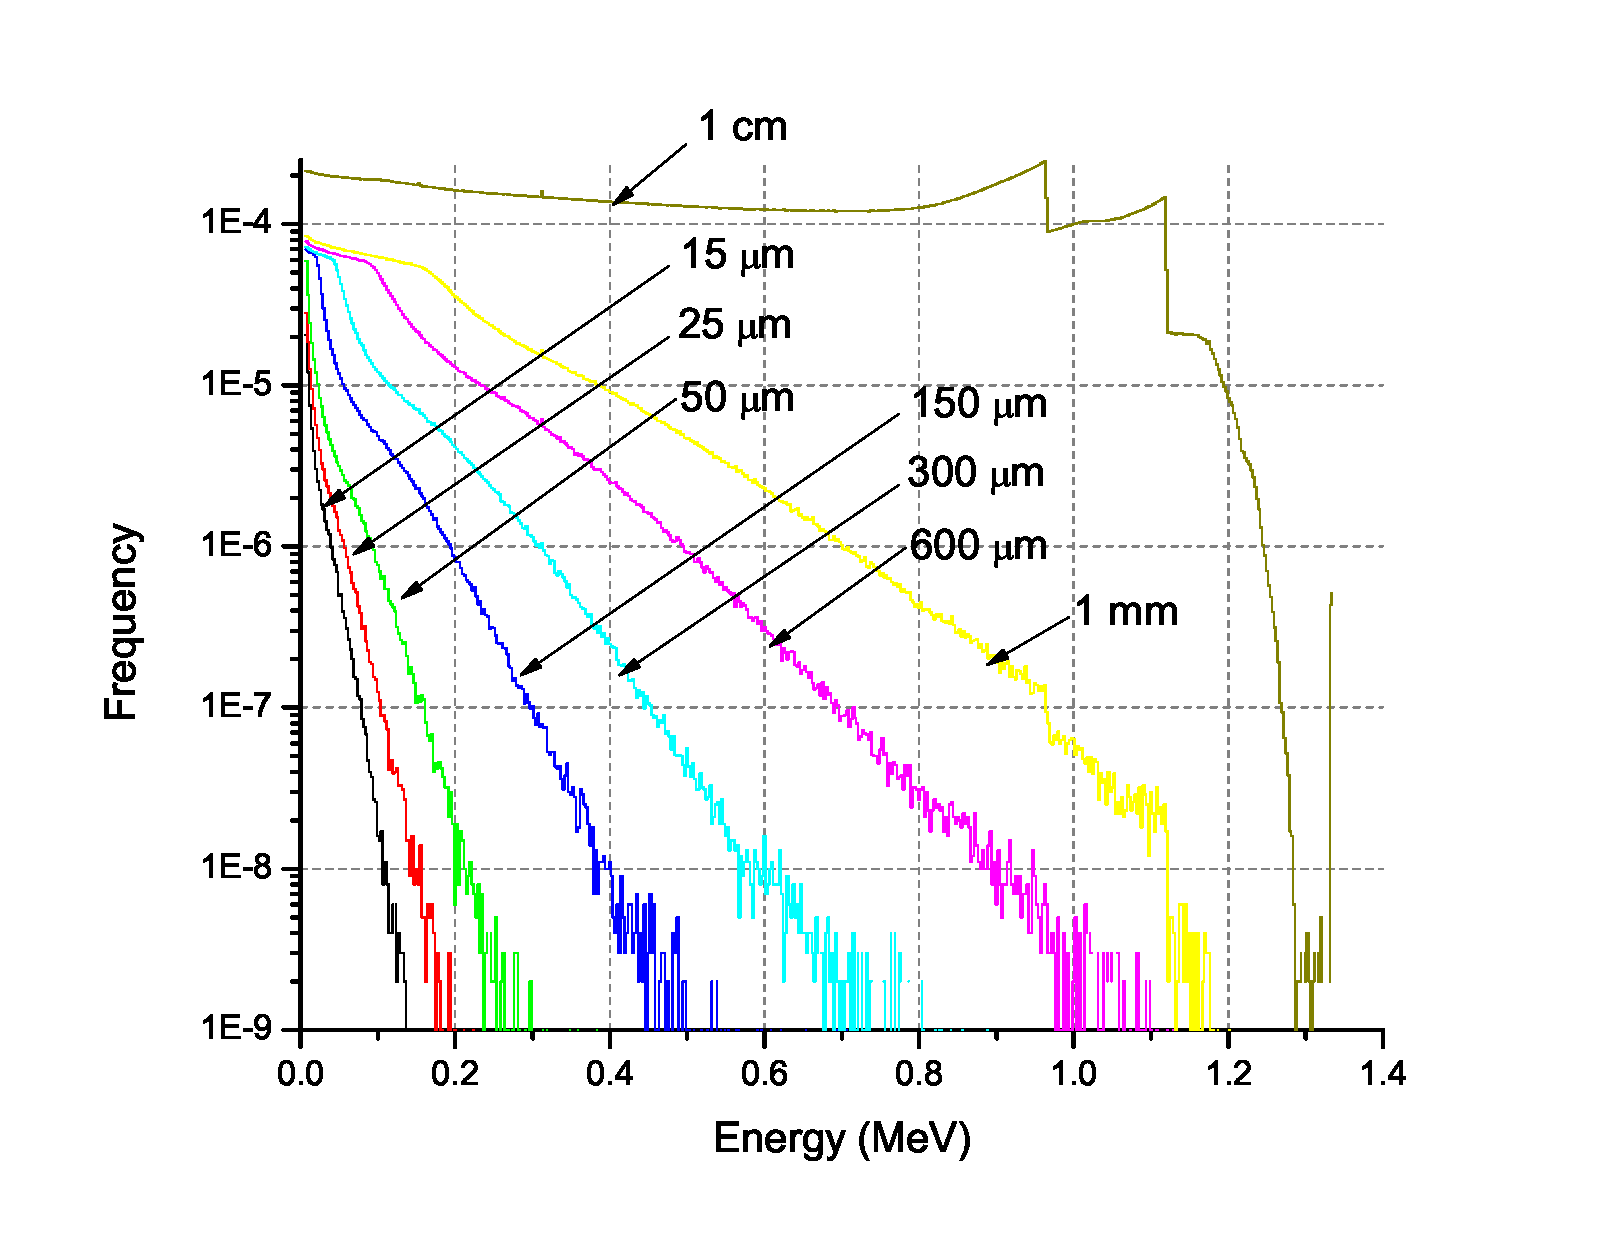
\includegraphics[width=\textwidth]{PS_EDepSim_Co60}
      \caption{Simulated}
    \end{figure}
  \end{column}
  \begin{column}{0.45\textwidth}
    \centering
    \begin{figure}
   	  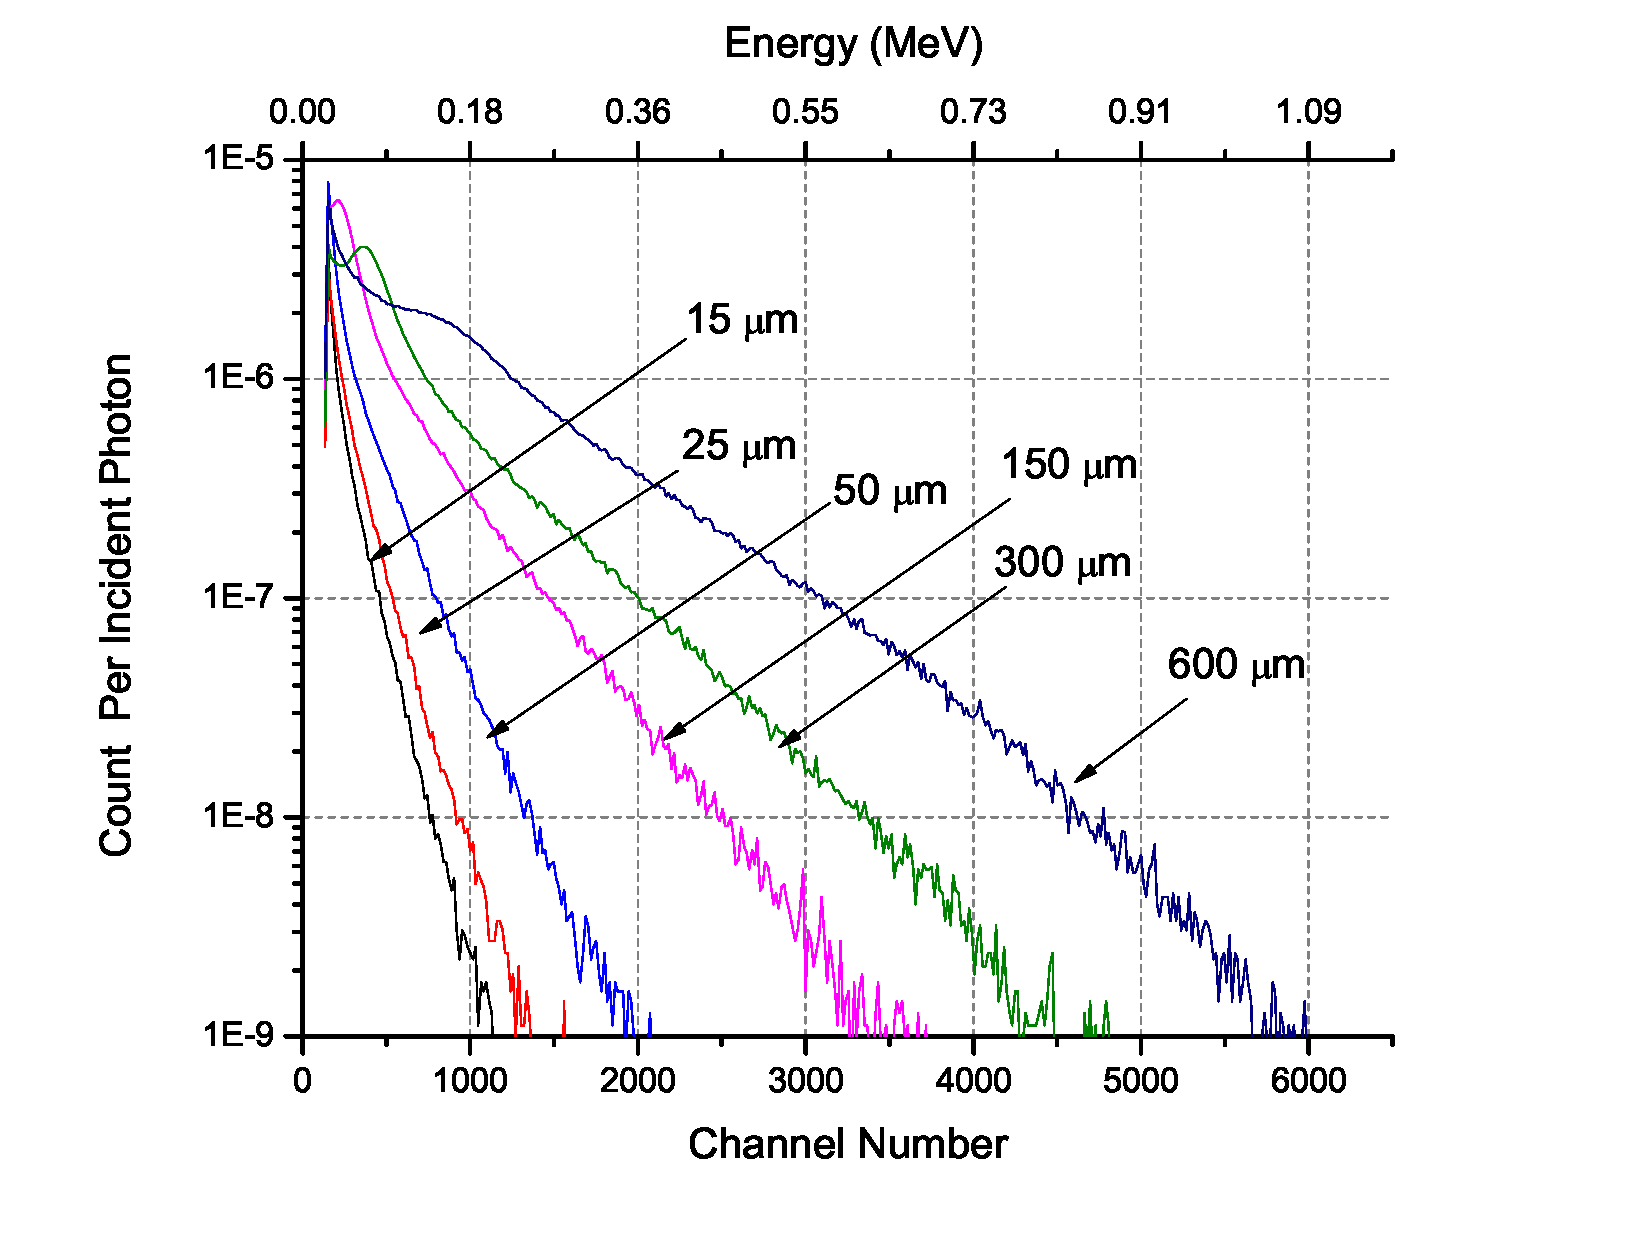
\includegraphics[width=\textwidth]{PS_GammaCR-Binned-FluxNorm_20LiF_5PPO}
      \caption{Simulated}
    \end{figure}
  \end{column}
  \end{columns}
\hyperlink{G4Main}{\beamerbutton{Return to Energy Deposition}}
\hyperlink{toc}{\beamerbutton{Table of Contents}}
\end{frame}
%%%%%%%%%%%%%%%%%%%%%%%%%%%%%%%%%%%%%%%%%%%%%%%%%%%%%%%%%%%%%%%%%%%%%%%%%%
\begin{frame}[fragile]{Optical Material Properties}
Most difficult part of simulation is correct properties
\begin{lstlisting}
void Materials::SetOpticalPropertiesGS20(){
    // Index of Reflection (146 nm to 1570 nm)
    const G4int nRINDEX = 13;
    G4double photonEnergyRINDEX[nRINDEX] = 
    {8.550*eV,4.723*eV,3.262*eV,2.492*eV,2.016*eV,
    1.692*eV,1.458*eV,1.281*eV,1.142*eV,1.031*eV, 
    0.939*eV,0.862*eV,0.797*eV};
    G4double RefractiveIndexGlass[nRINDEX]=
    {1.6508,1.5266,1.4980,1.4872,1.4819,    
    1.4790,1.4772,1.4760,1.4752,1.4746,    
    1.4742,1.4738,1.4736};
    // Absorbition Length
    const G4int nABS=2;
    G4double photonEnergyABS[nABS] = {3.5*eV,1.75*eV};
    G4double AbsLengthGlass[nABS] = {70*cm, 70*cm};  
\end{lstlisting}
\hyperlink{G4LightMain}{\beamerbutton{Return to Light Transport}}
\hyperlink{toc}{\beamerbutton{Table of Contents}}
\end{frame}
%%%%%%%%%%%%%%%%%%%%%%%%%%%%%%%%%%%%%%%%%%%%%%%%%%%%%%%%%%%%%%%%%%%%%%%%%%
\begin{frame}[fragile]{Optical Material Properties}
\begin{lstlisting}
    G4double photonEnergyEM[nEM] = {3.8,3.5,3.1,2.8,2.5};
    G4double emGS20[nEM]={0,0.19,0.37,0.32,0.10,0.02};
    MPTGS20->AddProperty("RINDEX",photonEnergyRINDEX,RefractiveIndexGlass,nRINDEX);
    MPTGS20->AddProperty("ABSLENGTH",photonEnergyABS,AbsLengthGlass,nABS);
	  MPTGS20->AddProperty("FASTCOMPONENT",photonEnergyEM,emGS20,nEM);
    MPTGS20->AddConstProperty("FASTTIMECONSTANT",50*ns);
    MPTGS20->AddConstProperty("SCINTILLATIONYIELD", 3600*MeV);
    MPTGS20->AddConstProperty("YIELDRATIO", 1.0);
    MPTGS20->AddConstProperty("RESOLUTIONSCALE", 1.0);
}
\end{lstlisting}
\hyperlink{G4LightMain}{\beamerbutton{Return to Light Transport}}
\hyperlink{toc}{\beamerbutton{Table of Contents}}
\end{frame}
%%%%%%%%%%%%%%%%%%%%%%%%%%%%%%%%%%%%%%%%%%%%%%%%%%%%%%%%%%%%%%%%%%%%%%%%%%

\section*{Genetic Algorthims}
\label{GAMethodExtended}
%% Genatic Algorthims introduction
%%%%%%%%%%%%%%%%%%%%%%%%%%%%%%%%%%%%%%%%%%%%%%%%%%%%%%%%%%%%%%%%%%%%%%%%%%
\begin{frame}{Genetic Algorithms}
A search technique mimicking natural evolution.
\begin{columns}[onlytextwidth]
  \begin{column}{0.45\textwidth}
    \small
    \begin{itemize}
      \item Population of candidate solutions is evolved toward better solutions
      \item Each candidate has properties that can be mutated and altered
      \item Traditionally solutions are represented as bit strings or trees
    \end{itemize}
    \end{column}
  \begin{column}{0.45\textwidth}
    \begin{figure}
		\tiny
		\begin{algorithmic}
      \WHILE{$error>goal$}
        \FORALL{$p \in P$}
          \STATE{Compute fitness}
        \ENDFOR
        \FORALL{$p \in P$}	
          \STATE{Choose individuals based on fitness}
          \STATE{Select individuals for next population}
          \STATE{Crossover selected individuals}
          \STATE{Mutate selected individual}
        \ENDFOR
      \ENDWHILE
    \end{algorithmic}
    \end{figure}
  \end{column}
\end{columns}
\hyperlink{GAMethod}{\beamerbutton{Return to Optimization}}
\hyperlink{toc}{\beamerbutton{Table of Contents}}
\end{frame}
%%%%%%%%%%%%%%%%%%%%%%%%%%%%%%%%%%%%%%%%%%%%%%%%%%%%%%%%%%%%%%%%%%%%%%%%%%
\begin{frame}{Crossover Operations}
	\begin{columns}[onlytextwidth]
	\begin{column}{0.4\textwidth}
  \begin{itemize}
    \item Single point - choose a single point (two segments) to crossover
    \item Two point - choose two points (three segments) to crossover
    \item Uniform - Uniformly cross over based on some probability
  \end{itemize}
	\end{column}
	\begin{column}{0.55\textwidth}
    \begin{figure}
      \centering
      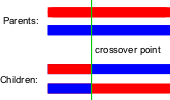
\includegraphics[width=0.3\textwidth]{SinglePointCrossover.png}
    \end{figure}
    \begin{figure}
      \centering
      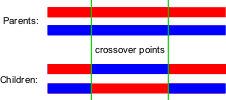
\includegraphics[width=0.3\textwidth]{TwoPointCrossover.png}
    \end{figure}
    \begin{figure}
      \centering
      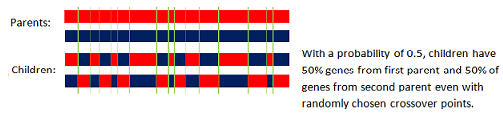
\includegraphics[width=\textwidth]{UniformCrossover.png}
    \end{figure}
	\end{column}
	\end{columns}
\hyperlink{GAMethod}{\beamerbutton{Return to Optimization}}
\hyperlink{toc}{\beamerbutton{Table of Contents}}
\end{frame}
%%%%%%%%%%%%%%%%%%%%%%%%%%%%%%%%%%%%%%%%%%%%%%%%%%%%%%%%%%%%%%%%%%%%%%%%%%
\begin{frame}{Mutation Operations}
Mutations are designed to avoid local minima
\begin{columns}
\begin{column}{0.45\textwidth}
  \begin{itemize}
    \item Swap
    \item Flip - flips (inverts) all of the bits
  \end{itemize}
    \begin{figure}
      \centering
      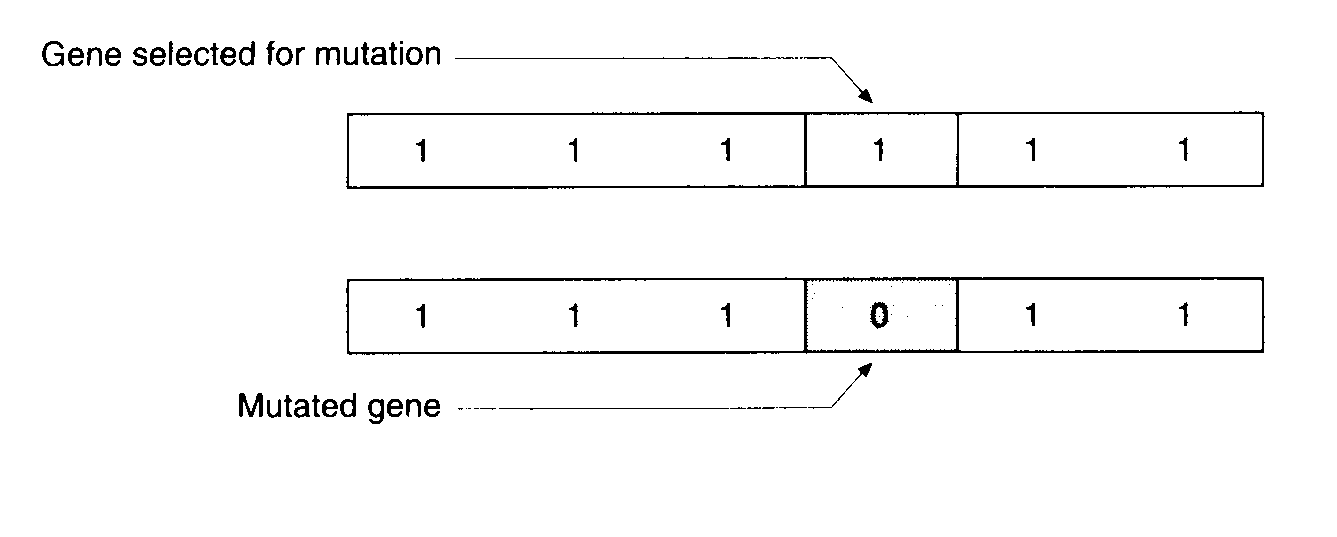
\includegraphics[width=0.4\textheight]{mutation_example.png}
    \end{figure}
	Typically set to be around a few percent
\end{column}
\begin{column}{0.45\textwidth}
\begin{figure}
	\centering
	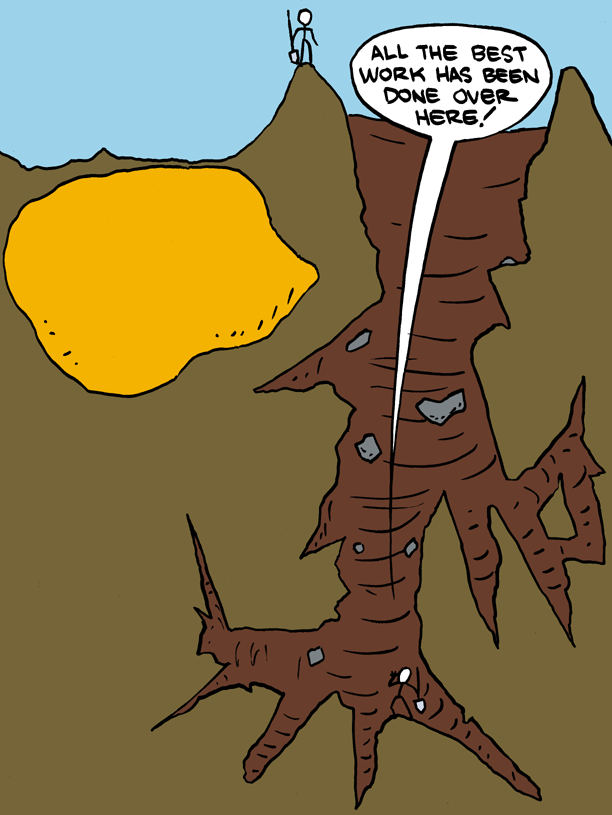
\includegraphics[width=0.75\textwidth]{AllTheBestWork.png}
\end{figure}
\end{column}
\end{columns}
\hyperlink{GAMethod}{\beamerbutton{Return to Optimization}}
\hyperlink{toc}{\beamerbutton{Table of Contents}}
\end{frame}
%%%%%%%%%%%%%%%%%%%%%%%%%%%%%%%%%%%%%%%%%%%%%%%%%%%%%%%%%%%%%%%%%%%%%%%%%%
\begin{frame}{Fitness Function}
The fitness function was chosen to count rate per mass of \iso[6]{Li}, provided that the geometry meet the total count rate criteria.
If it failed to meet the count rate criteria a zero fitness was returned \eqref{eqn:FitnessFun}.
	\tiny
	\begin{align}
			\label{eqn:FitnessFun}
			f(\vec{x})
			= \begin{cases}
			0 & \text{if}~\text{countRate}(\vec{x}) \leq \SI{2.5}{cps\per\nano\gram\iso[252]{Cf}} \\
			\text{countRatePerMass}(\vec{x}) & \text{otherwise}
			\end{cases}
	\end{align}
\begin{columns}[onlytextwidth]
  \begin{column}{0.5\textwidth}
\small
	Computationally intensive to calculate the fitness function 
	\begin{itemize}
		\item Memoization with dictionaries
		\item Multithreading for items not in the dictionary
		\tiny
		\begin{itemize}
			\item This made it sensitive while running
			\item Future work would be to use the PyEvovle multithreading option
		\end{itemize}
	\end{itemize}
	\end{column}
	\begin{column}{0.4\textwidth}
    \begin{figure}
      \centering
      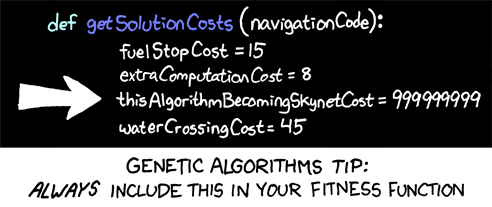
\includegraphics[width=\textwidth]{genetic_algorithms}
    \end{figure}
	\end{column}
\end{columns}
\hyperlink{GAMethod}{\beamerbutton{Return to Optimization}}
\hyperlink{toc}{\beamerbutton{Table of Contents}}
\end{frame}

\end{document}


